% Modified for use with JCC - Madhusudan Singh Copyright (C) (2012). All rights reserved.
\documentclass[12pt]{article}

\setlength{\oddsidemargin}{0in}  %left margin position, reference is one inch
\setlength{\textwidth}{6.5in}    %width of text=8.5-1in-1in for margin
\setlength{\topmargin}{-0.5in}    %reference is at 1.5in, -.5in gives a start of about 1in from top
\setlength{\textheight}{9in}     %length of text=11in-1in-1in (top and bot. marg.) 
\newenvironment{wileykeywords}{\textsf{Keywords:}\hspace{\stretch{1}}}{\hspace{\stretch{1}}\rule{1ex}{1ex}}

\usepackage{amsmath,amssymb}
\usepackage{graphicx}% Include figure files
%\usepackage{caption}
\usepackage{color}% Include colors for document elements
\usepackage{dcolumn}% Align table columns on decimal point
\usepackage{bm}% bold math
\usepackage[numbers,super,comma,sort&compress]{natbib}
\usepackage{multirow}
%\usepackage[nolists, nomarkers, figuresfirst]{endfloat}


\usepackage{hyperref}


\definecolor{background-color}{gray}{0.98}

\title{Coupling finite and boundary element methods to solve the Poisson-Boltzmann equation for electrostatics in molecular solvation}
\author{Micha\l{} Bosy\thanks{School of Computer Science and Mathematics, Kingston University London, Penrhyn Road, Kingston upon Thames, KT1 2EE, UK}, Matthew W. Scroggs\thanks{Department of Mathematics, University College London, 25 Gordon Street, WC1H 0AY London, UK}, Timo Betcke\thanks{Department of Mathematics, University College London, 25 Gordon Street, WC1H 0AY London, UK}, Erik Burman\thanks{Department of Mathematics, University College London, 25 Gordon Street, WC1H 0AY London, UK}, Christopher D. Cooper\thanks{Department of Mechanical Engineering and Centro Cient\'ifico Tecnol\'ogico de Valpara\'iso, Universidad T\'ecnica Federico Santa Mar\'ia, Valpara\'iso 2390123, Chile}}

\begin{document}

\maketitle


\begin{abstract}
Abstract
\end{abstract}

\begin{wileykeywords}
Finite element method, Boundary element method, Poisson-Boltzmann, Implicit solvent model, Electrostatics.
\end{wileykeywords}

\clearpage

%*****************Graphical Table of Contents******************** THIS IS MANDATORY *******************


\begin{figure}[h]
\centering
\colorbox{background-color}{
\fbox{
\begin{minipage}{1.0\textwidth}
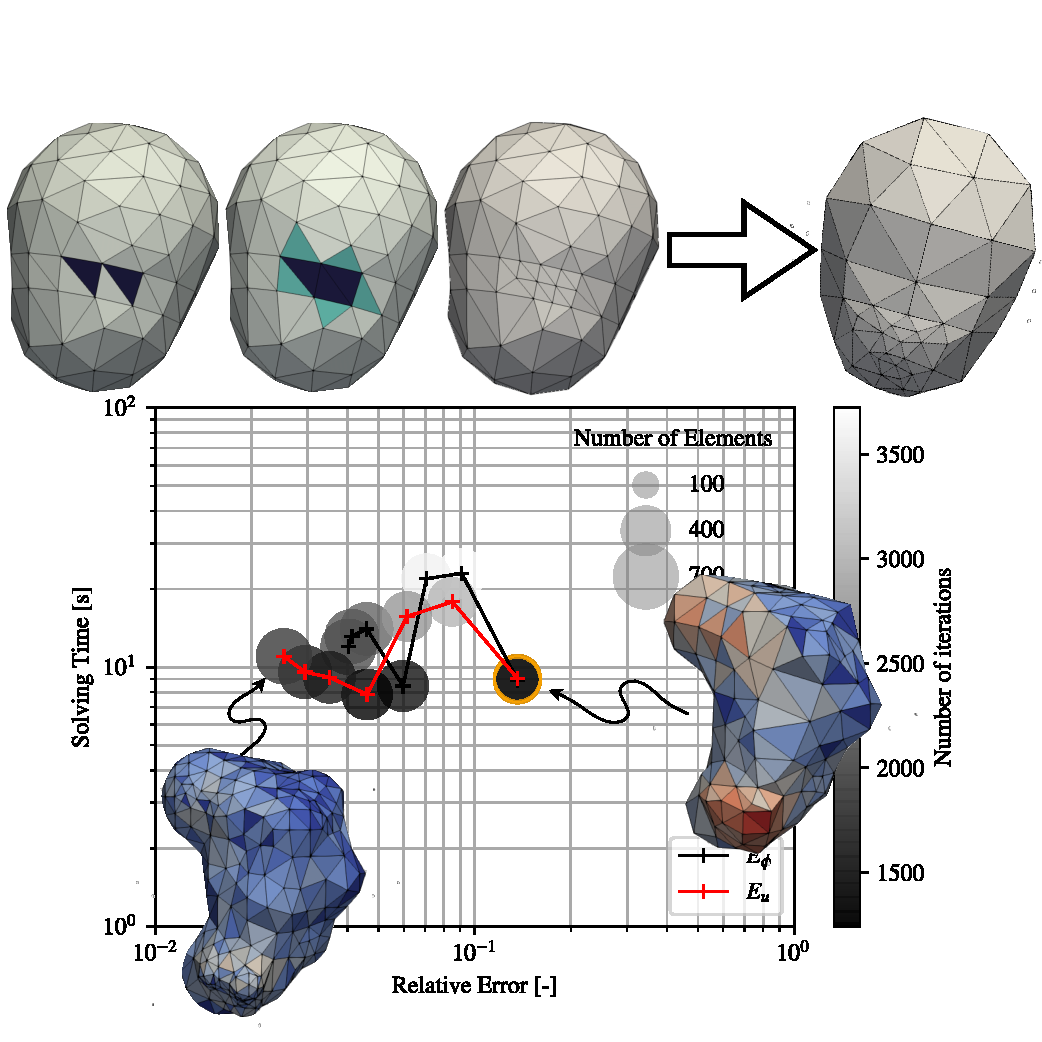
\includegraphics[width=50mm,height=50mm]{adaptive_mesh_fig.pdf} %Pick only one of the two styles by uncommenting the corresponding \includegraphics
%\includegraphics[width=110mm,height=20mm]{cc.eps}
\\
(75 words.) Images for the graphical Table of Contents should capture the essence of a paper, displaying a figure, plot, or scheme that is central to the theme of the manuscript. The text of the graphical Table of Contents is meant for the non-specialist and should ideally contain no obscure jargon or mathematical symbols / equations, but should attempt to convey the gist of the paper in everyday terms, while remaining consistent with accepted standards of scientific literature.
\end{minipage}
}}
\end{figure}

% makes references listed with 1., 2., etc.  
  \makeatletter
  \renewcommand\@biblabel[1]{#1.}
  \makeatother

\bibliographystyle{apsrev}

\renewcommand{\baselinestretch}{1.5}
\normalsize


\clearpage


\section*{\sffamily \Large INTRODUCTION} % Not needed for rapid communications

In biologically relevant settings, the structure and function of biomolecules is largely determined by the surrounding water, which usually contains salt. 
To describe these systems accurately, we need to account for the solvent correctly, which has given rise to a wide range of models \cite{onufriev2018water}
Highly detailed models consider every water molecule and salt ion explicitly, however, there are approximated models that use continuum theory to represent this ionic solution, knwon as implicit-solvent models\cite{RouxSimonson1999,DecherchiETal2015}.
In the case of electrostatics, the implicit-solvent model is mathematically characterized by the Poisson-Boltzmann equation (PBE)\cite{Baker2004,Bardhan2012}, which is widely used to compute solvation free energies and mean-field potentials.

The implicit-solvent model for electrostatics describes the dissolved molecule as a infinite medium with a low-dielectric solute-shaped cavity, which contains a charge distribution from the partial charges --- usually a sum of Dirac deltas at the atom's locations.
The outer solvent region is represented with a high dielectric, and considers the presence of salt.
These two regions are interfaced by the molecular surface, which can be defined in various ways \cite{HarrisBoschitcshFenley2013}, where the continuity of the electrostatic potential and electric displacement are enforced.

The PBE has been solved numerically with finite difference\cite{BakerETal2001,GilsonETal1985,JurrusETal2018,LiETal2019}, finite element\cite{HolstETal2012,BondEtal2010}, boundary element\cite{AltmanBardhanWhiteTidor09,LuETal2006,GengKrasny2013,CooperBardhanBarba2014}, and analytical\cite{YapHeadgordon2010,FelbergETal2017} methods.
In particular, the boundary element method (BEM) has proven to be very efficient for high accuracy calculations [GengKrasny2013,CooperBardhanBarba2014], mainly due to the precise description of the molecular surface and point charges. 
However, BEM is limited to constant material properties in each region, and the linear version of the PBE. 
Even though these limitations are acceptable in a wide range of applications, there are cases when BEM falls short, for example, if a variable permittivity is required inside the solute [cite], or the solute is highly charged such that the linear approximation breaks [cite?].

This article presents a methodology to overcome some of those limitations, through coupling boundary and finite elements (FEM-BEM).
This approach brings the best of both worlds: the flexibility of FEM and efficiency of BEM, all in an accurate description of the dissolved molecule.


% The opening sentence of the manuscript should summarize the reasons for the undertaking of the work and the main conclusions that can be drawn.

%((Place Introduction here))

%((Main text paragraphs should be 12 point font, double-spaced. Reviews are comprehensive survey of recent progress in a topic of broad interest in quantum chemistry, providing the readership with an appreciation of the importance of the work, a summary of recent developments, and a guide to the relevant literature. Perspective are short discussions of an important emerging topics in quantum chemistry, usually focused on no more than a few recently published papers, and including the authors' vision for the future of the topics, identifying important problems that should be addressed next. Perspective should be limited to 3000 words, 4 display items (figures and/or tables), and 30 references.))

%((Full Papers are comprehensive reports of important recent advances in the development of basic theory, quantum mechanical computational methodologies and their relevant applications that provide significant insight to problems of broad interest in chemistry, physics, biology, and materials science. The opening sentence of the manuscript should summarize the reasons for the undertaking of the work and the main conclusions that can be drawn. The main text should be contain sections with brief subheadings, a summary of the major conclusions of the paper, and a Method section containing sufficient detail to reproduce the work. Main text paragraphs should be 12 point font, double-spaced.))

%((Rapid communications should be limited to 1500 words, 3 display items (figure and/or tables), 20 references. Main text paragraphs should be 12 point font, double-spaced. There are NO headings in the main text.))

\section*{\sffamily \Large METHODOLOGY}
\subsection*{\sffamily \large The implicit solvent model}

The implicit solvent model\cite{RouxSimonson1999,DecherchiETal2015} can be described mathematically as a coupled system of partial differential equations, where the Poisson-Boltzmann governs in the solvent region ($\Omega_1$ in Figure \ref{fig:implicit_molecule}), and the Poisson equation in the solute region ($\Omega_2$ in Figure \ref{fig:implicit_molecule}). These regions are interfaced by the molecular surface ($\Gamma$), where the potential ($\phi$) and electric displacement ($\epsilon\partial\phi/\partial\mathbf{n}$) are continuous. 
%
\begin{align}\label{eq:pbe}
\nabla^2\phi_1(\mathbf{x}) &= \tfrac{1}{\epsilon_1}\sum_{k=1}^{N_q} q_k\delta(\mathbf{x},\mathbf{x}_k) \quad  \mathbf{x} \in \Omega_1\nonumber\\
\left(\nabla^2 - \kappa^2\right)\phi_2(\mathbf{x})  &= 0 \quad\mathbf{x}\in\Omega_2\nonumber\\
\phi_1(\mathbf{x})  = \phi_2 (\mathbf{x}), &\quad \epsilon_1\frac{\partial\phi_1}{\partial\mathbf{n}}(\mathbf{x})  = \epsilon_2\frac{\partial\phi_2}{\partial\mathbf{n}}(\mathbf{x})  \quad \mathbf{x}\in \Gamma. 
\end{align}
%
Here, $\epsilon_1$ and $\epsilon_2$ are the dielectric constants in the solute and solvent, respectively, $\kappa$ is the inverse of the Debye length, related with the salt concentration, and $q_k$ are the values of the partial charges, located at $\mathbf{x}_k$.

\begin{figure}[h]
\centering
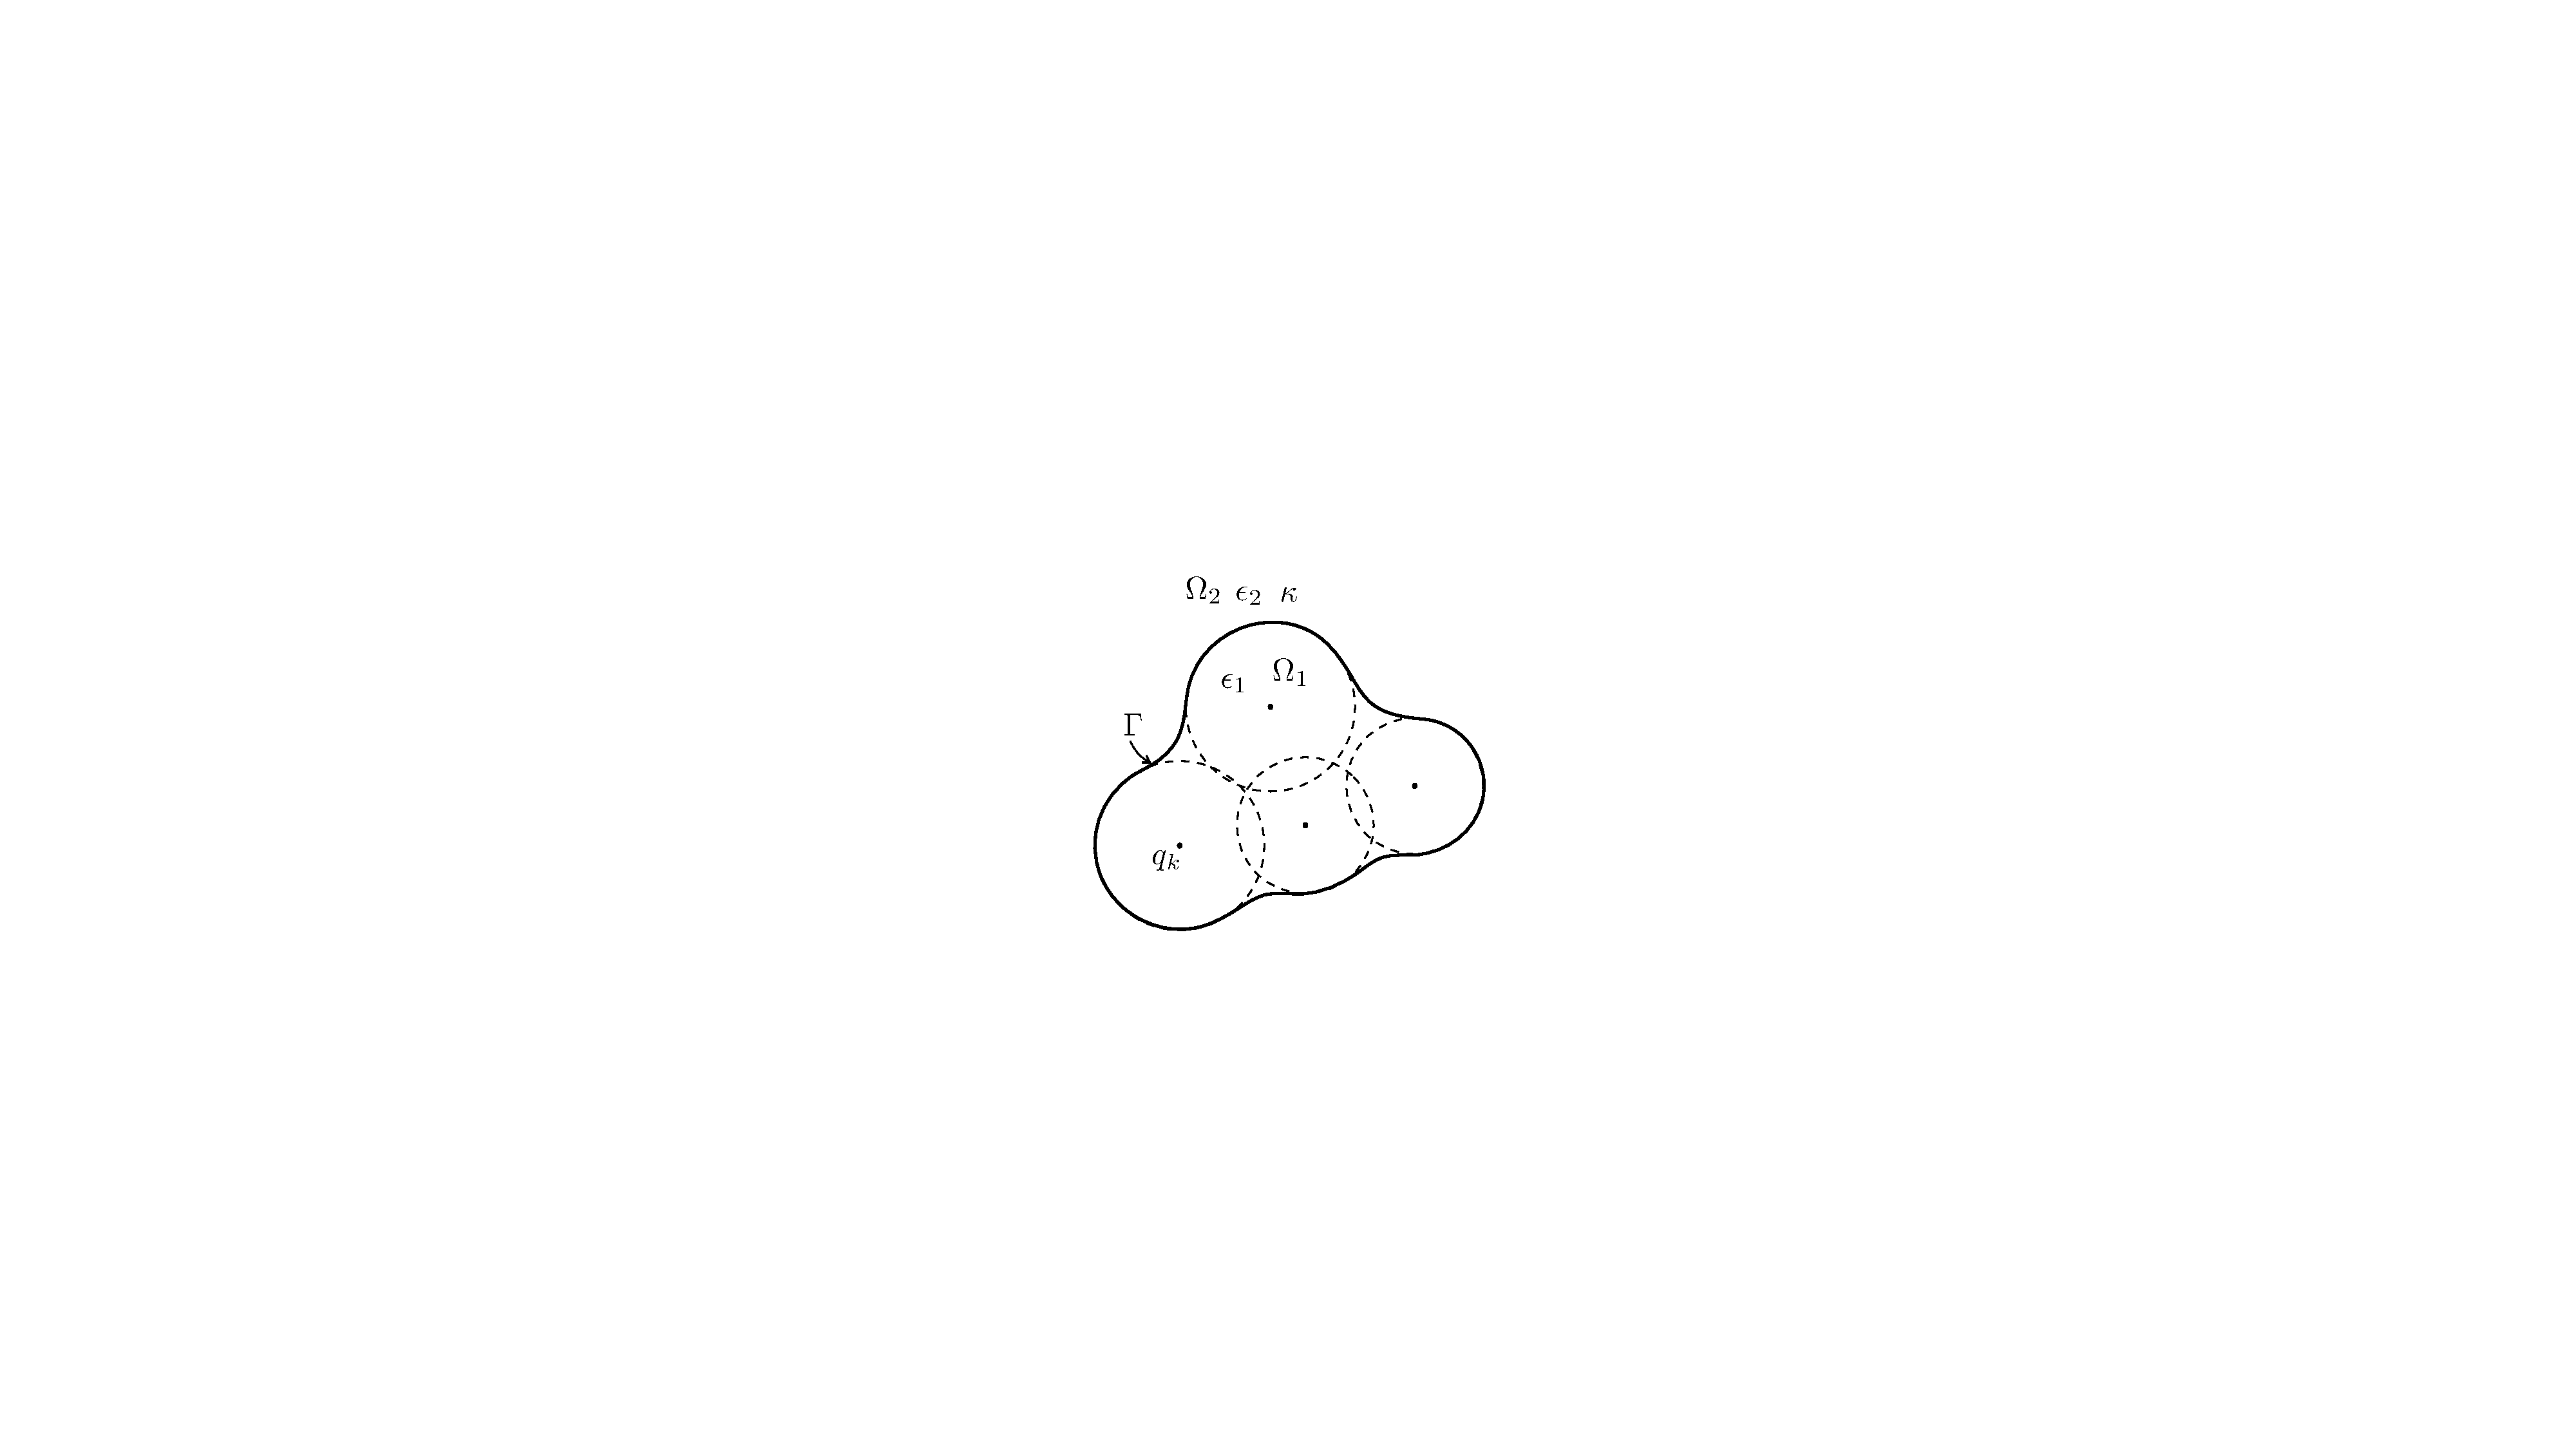
\includegraphics[width=0.3\textwidth]{implicit_molecule.pdf}
\caption{Representation of a molecule in an implicit solvent.}
\label{fig:implicit_molecule}
\end{figure}

The electrostatic potential in $\Omega_1$ can be further decomposed into singular and regular components as $\phi_1 = \phi_c + \phi_r$, where $\phi_c$ is the solution to
%
\begin{align}\label{eq:phic}
\nabla^2\phi_c(\mathbf{x}) &= \tfrac{1}{\epsilon}\sum_{k=1}^{N_q}q_k\delta(\mathbf{x},\mathbf{x}_k) \quad \mathbf{x}\in\Omega_1\cup\Omega_2\nonumber\\
\phi_c(\mathbf{x})&=0 \quad \text{ as } |\mathbf{x}|\to\infty
\end{align}

Physically, $\phi_c$ can be interpreted as the Coulomb-type potential from the point charges, whereas $\phi_r$, also known as reaction potential, is originated by the polarization of the solvent and reorganization of the free ions. 
Usually, $\epsilon_1$ is considered a constant value, yielding an analytical expression for $\phi_c$, however, this is not the general case.

Regularized versions of Equation \eqref{eq:pbe} \cite{LuZhouHolstMcCammon2008,LeeGengZhao2021} are widely used to numerically solve the Poisson-Boltzmann equation with finite element or finite difference methods, and have recently been extended to super-Gaussian permitivitties in the solute.\cite{wang2022regularization} However, here we use the standard formulation in Equation \eqref{eq:pbe}, as it offers more flexibility when dealing with, for example, variable permitivitties, beyond super-Gaussian descriptions.

A common quantity of interest in implicit solvent models is the solvation free energy, which the change in Gibbs free energy as the molecule moves from vacuum into the solvent. Considering the charge distribution $\rho$ consists of point charges, this can be calculated as
%
\begin{equation}\label{eq:dG} 
\Delta G_{solv} = \tfrac{1}{2}\int_{\Omega_1} \rho(\mathbf{x})\phi_{r}(\mathbf{x}) = \tfrac{1}{2}\sum_{k=1}^{N_q} q_k\phi_r(\mathbf{x_k})
\end{equation}

\subsection*{\sffamily \large BEM-BEM coupling}

Several possible boundary integral formulations of Equation \eqref{eq:pbe} exist.~\cite{search2022towards} The simplest form was presented by Yoon ºand Lenhoff in 1991,~\cite{YoonLenhoff1990} known as the \emph{direct} formulation, however, the resulting system is usually ill-conditioned. Here, we use the better-conditioned formulation presented by Lu and co-workers,~\cite{LuETal2006,LuETal2009,debuhr2016dashmm} which reads
%
\begin{align}\label{eq:lu}
    & \tfrac{\phi_2}{2}\left(1+\tfrac{\epsilon_1}{\epsilon_2}\right) - \left(K_Y^\Gamma - \tfrac{\epsilon_1}{\epsilon_2}K_L^\Gamma\right)\phi_2 + \left(V_Y^\Gamma - V_L^\Gamma\right)\lambda_2 = \sum_{k=0}^{N_q}  \frac{q_k}{4\pi\epsilon_2|\mathbf{x}_{\Gamma} - \mathbf{x}_k|}
     \nonumber \\
    &\tfrac{\epsilon_1}{\epsilon_2}\left(W_Y^\Gamma - W_L^\Gamma\right)\phi_2 +  \tfrac{\lambda_2}{2}\left(1+\tfrac{\epsilon_1}{\epsilon_2}\right) + \left(\tfrac{\epsilon_1}{\epsilon_2}K_Y^{\prime\Gamma} - K_L^{\prime\Gamma}\right)\lambda_2 = \sum_{k=0}^{N_q}  \frac{\partial}{\partial\mathbf{n}_\mathbf{x}}\left(\frac{q_k}{4\pi\epsilon_2|\mathbf{x}_{\Gamma} - \mathbf{x}_k|}\right)
\end{align}
\textcolor{blue}{Michal: We only have $\phi_2$ and $\lambda_2$ and the solution later is from $\phi_1$ and $\lambda_1$!!!}


%
In Equation \eqref{eq:lu}, $\phi_1 = \phi_1(\mathbf{x}_\Gamma)$ and $\phi_2 = \phi_2(\mathbf{x}_\Gamma)$ are the potentials on $\Gamma$ as we approach from $\Omega_1$ and $\Omega_2$, respectively. For convenience, we call the normal derivative on the interface ({\it ie.} the Neumann trace) $\lambda=\left(\frac{\partial}{\partial \mathbf{n}}  \phi_{\Gamma}  \right)$. $V$, $K$, $K^{\prime}$, and $W$ are the single-layer, double-layer, adjoint double-layer, and hypersingular operators for the Laplace (subscript $L$) and Yukawa (subscript $Y$, also known as modified Helmholtz) kernels. These are defined %in Equation~\eqref{eq:single_double} and 
as
%
\begin{align}\label{eq:all_op}
V_i^\Gamma \varphi (\mathbf{x}) &= \oint_\Gamma g_i(\mathbf{x},\mathbf{x}')\varphi(\mathbf{x}')d\mathbf{x}'\nonumber\\
K_i^\Gamma \varphi (\mathbf{x}) &= \oint_\Gamma \frac{\partial g_i}{\partial\mathbf{n}'}(\mathbf{x},\mathbf{x}')\varphi(\mathbf{x}')d\mathbf{x}',\nonumber\\
K^{\prime\Gamma}_i\varphi (\mathbf{x}) &= \oint_\Gamma \frac{g_i}{\partial\mathbf{n}}(\mathbf{x}_\Gamma,\mathbf{x}')\varphi(\mathbf{x}')d\mathbf{x}'\nonumber\\
W^\Gamma_i\varphi (\mathbf{x}) &= - \oint_\Gamma \frac{\partial^2 g_i}{\partial\mathbf{n}'\partial\mathbf{n}}(\mathbf{x}_\Gamma,\mathbf{x}')\varphi(\mathbf{x}')d\mathbf{x}'
\end{align}
%
where $i \in \{L,Y\}$, $\varphi(\mathbf{x})$ can be any distribution over $\Gamma$, and %Green's functions $g_L, g_Y$ were defined in Equation~\eqref{eq:green_func}.
\begin{align}\label{eq:green_func}
g_L(\mathbf{x},\mathbf{x}')=\frac{1}{4\pi|\mathbf{x}-\mathbf{x}'|} \nonumber \\
g_Y(\mathbf{x},\mathbf{x}')=\frac{e^{-\kappa|\mathbf{x}-\mathbf{x}'|}}{4\pi|\mathbf{x}-\mathbf{x}'|}
\end{align}
are the corresponding free-space Green's functions.

%%Applying Green's second identity to Equation \eqref{eq:pbe} we get 
%%
%%\begin{align} \label{eq:volume_potential}
%%\phi_{1}(\mathbf{x}_{\Omega_1})+ K_{L}^{\Omega_1}\phi_1 -  V_{L}^{\Omega_1} \lambda_2^1 & = \tfrac{1}{\epsilon_1} \sum_{k=0}^{N_q}  \frac{q_k}{4\pi|\mathbf{x}_{\Omega_1} - \mathbf{x}_k|}  \quad \text{on $\Omega_1$,} \nonumber \\
%%\phi_{2}(\mathbf{x}_{\Omega_2}) - K_{Y}^{\Omega_2}\phi_2 + \tfrac{\epsilon_1}{\epsilon_2} V_{Y}^{\Omega_2} \lambda_2& = 0 \quad \text{on $\Omega_2$,}
%%\end{align}
%%
%%where $\mathbf{x}_\Omega$ is evaluated anywhere in the correspoding domain, except $\Gamma$, and $\phi_1 = \phi_1(\mathbf{x}_\Gamma)$ and $\phi_2 = \phi_2(\mathbf{x}_\Gamma)$ are the potentials on $\Gamma$ as we approach from $\Omega_1$ and $\Omega_2$, respectively. For convenience, we call the normal derivative on the interface ({\it ie.} the Neumann trace) $\lambda=\left(\frac{\partial}{\partial \mathbf{n}}  \phi_{\Gamma}  \right)$. $K$ and $V$ are the double- and single-layer potentials for the Laplace (subscript $L$) and Yukawa (subscript $Y$, also known as modified Helmholtz) kernels
%%
%%\begin{align}\label{eq:single_double}
%%V^D \varphi (\mathbf{x}) = \oint_\Gamma g_i(\mathbf{x},\mathbf{x}')\varphi(\mathbf{x}')d\mathbf{x}'\nonumber\\
%%K^D \varphi (\mathbf{x}) = \oint_\Gamma \frac{\partial g_i}{\partial\mathbf{n}'}(\mathbf{x},\mathbf{x}')\varphi(\mathbf{x}')d\mathbf{x}',\nonumber\\
%%\end{align}
%%
%%where $D \in \{\Omega_1, \Omega_2, \Gamma\}$, $i \in \{L,Y\}$, $\varphi(\mathbf{x})$ can be any distribution over $\Gamma$, and 
%%
%%\begin{align}\label{eq:green_func}
%%g_L(\mathbf{x},\mathbf{x}')=\frac{1}{4\pi|\mathbf{x}-\mathbf{x}'|} \nonumber \\
%%g_Y(\mathbf{x},\mathbf{x}')=\frac{e^{-\kappa|\mathbf{x}-\mathbf{x}'|}}{4\pi|\mathbf{x}-\mathbf{x}'|}
%%\end{align}
%%
%%are the free-space Green's function of the Laplace and linearized Poisson-Boltzmann equations, respectively. 
%
%%If we take the limit of Eq. \eqref{eq:volume_potential} as $\mathbf{x}_{\Omega}$ approaches $\Gamma$, we get
%%
%%\begin{align} \label{eq:direct}
%%\tfrac{\phi_1}{2}+ K_{L}^{\Gamma}\phi_1 -  V_{L}^{\Gamma} \lambda_2^1 & = \tfrac{1}{\epsilon_1} \sum_{k=0}^{N_q}  \frac{q_k}{4\pi|\mathbf{x}_{\Gamma} - \mathbf{x}_k|} \nonumber \\
%%\tfrac{\phi_2}{2} - K_{Y}^{\Gamma}\phi_2 +  \tfrac{\epsilon_1}{\epsilon_2} V_{Y}^{\Gamma} \lambda_2 & = 0
%%\end{align}
%%
%%The {\it direct} formulation\cite{YoonLenhoff1990} couples the two expressions of Eq. \eqref{eq:direct} on $\Gamma$, considering the interface conditions. Even though this formulation is poorly conditioned with respect to the mesh size, it can still model large systems when it is preconditioned appropriately.\cite{AltmanBardhanWhiteTidor09,MartinezETal2019,wang2021high} 
%%The formulation presented by Lu\cite{LuETal2006} takes the normal derivative of \eqref{eq:direct} to couple both $\phi$ and $\partial\phi/\partial\mathbf{n}$ as
%%
%%\begin{align}\label{eq:lu}
%%    & \tfrac{\phi_2}{2}\left(1+\tfrac{\epsilon_1}{\epsilon_2}\right) - \left(K_Y^\Gamma - \tfrac{\epsilon_1}{\epsilon_2}K_L^\Gamma\right)\phi_2 + \left(V_Y^\Gamma - V_L^\Gamma\right)\lambda_2 = \sum_{k=0}^{N_q}  \frac{q_k}{4\pi\epsilon_2|\mathbf{x}_{\Gamma} - \mathbf{x}_k|}
%%     \nonumber \\
%%    &\tfrac{\epsilon_1}{\epsilon_2}\left(W_Y^\Gamma - W_L^\Gamma\right)\phi_2 +  \tfrac{\lambda_2}{2}\left(1+\tfrac{\epsilon_1}{\epsilon_2}\right) + \left(\tfrac{\epsilon_1}{\epsilon_2}K_Y^{\prime\Gamma} - K_L^{\prime\Gamma}\right)\lambda_2 = \sum_{k=0}^{N_q}  \frac{\partial}{\partial\mathbf{n}_\mathbf{x}}\left(\frac{q_k}{4\pi\epsilon_2|\mathbf{x}_{\Gamma} - \mathbf{x}_k|}\right)
%%\end{align}
%%
%%The two new integral operators that appear are defined as 
%%
%%\begin{align}
%%\label{eq:adj_hyp}
%%K^{\prime\Gamma}_i\varphi (\mathbf{x}) = \oint_\Gamma \frac{g_i}{\partial\mathbf{n}}(\mathbf{x}_\Gamma,\mathbf{x}')\varphi(\mathbf{x}')d\mathbf{x}'\nonumber\\
%%W^\Gamma_i\varphi (\mathbf{x}) = - \oint_\Gamma \frac{\partial^2 g_i}{\partial\mathbf{n}'\partial\mathbf{n}}(\mathbf{x}_\Gamma,\mathbf{x}')\varphi(\mathbf{x}')d\mathbf{x}'
%%\end{align}
%%where $i \in \{L,Y\}$, 
%%and are called the {\it  adjoint double layer} and {\it hypersingular} operators, respectively. Note that the potential in Eq. \eqref{eq:lu} is evaluated on the exterior. 
%
%In weak form, Eq. \eqref{eq:lu} becomes
%%
%\begin{align}\label{eq:lu_disc}
%&\left< \left(1+\tfrac{\epsilon_1}{\epsilon_2}\right) \tfrac{\phi_{2}}{2} - \left(K_Y^\Gamma - \tfrac{\epsilon_1}{\epsilon_2}K_L^\Gamma\right)\phi_{2}, v \right>_{\Gamma} + \left< \left(V_Y^\Gamma - V_L^\Gamma\right) \lambda_2, v \right>_\Gamma = \left< \sum_{k=0}^{N_q}  f_k, v \right>_{\Gamma} \nonumber \\
%&\left< \tfrac{\epsilon_1}{\epsilon_2}\left(W_Y^\Gamma - W_L^\Gamma\right)\phi_{2}, \zeta \right>_\Gamma + \left<  \left(1+\tfrac{\epsilon_1}{\epsilon_2}\right) \tfrac{\lambda_2}{2} + \left(\tfrac{\epsilon_1}{\epsilon_2}K_Y^{\prime\Gamma} - K_L^{\prime\Gamma}\right)\lambda_2, \zeta\right>_\Gamma = \left< \sum_{k=0}^{N_q}  \frac{\partial}{\partial\mathbf{n}_\mathbf{x}} f_k, \zeta \right>_{\Gamma}
%\end{align}
%%
%where $v, \zeta$ are test functions, $\left<\varphi,v\right>_\Gamma = \int_\Gamma \varphi(\mathbf{x})v(\mathbf{x})d\mathbf{x}$ %and $\left(\varphi,v\right)_\Omega = \int_\Omega \varphi(\mathbf{x})v(\mathbf{x})d\mathbf{x}$ are 
%is the inner products on the surface% and domain, respectively
%and $f_k := \frac{q_k}{4\pi\epsilon_2|\mathbf{x}_{\Gamma} - \mathbf{x}_k|}$.
%
%We introduce below the matrix formulation. Let $\vec{\phi}_2 := [\phi_2^1, \dots, \phi_2^k]^T$ be the vector of canonical basis
%functions of $W_{h}^{k}$ and  $\vec{\lambda}_2 := [\lambda_2^1, \dots, \lambda_2^l]^T$ - the vector of canonical basis
%functions of $\Lambda_{h}^{l}$. We define the following matrices associated with the corresponding bilinear forms
%\begin{align*}
%\widetilde{K}_{\alpha \beta} = \left<\left(K_Y^\Gamma - \tfrac{\epsilon_1}{\epsilon_2}K_L^\Gamma\right) \phi^{\alpha}_2, \ \lambda^{\beta}_2 \right>_{\Gamma}
% &,&
%\widetilde{V}_{\alpha \beta} = \left<\left(V_Y^\Gamma - V_L^\Gamma\right) \lambda^{\alpha}_2, \ \lambda^{\beta}_2 \right>_{\Gamma}, \\
%\widetilde{W}_{\alpha \beta} = \left<\left(W_Y^\Gamma - W_L^\Gamma\right) \phi^{\alpha}_2, \ \phi^{\beta}_2 \right>_{\Gamma}
% &,&
%\widetilde{K'}_{\alpha \beta} = \left<\left(\tfrac{\epsilon_1}{\epsilon_2}K_Y^{\prime\Gamma} - K_L^{\prime\Gamma}\right) \lambda^{\alpha}_2, \ \phi^{\beta}_2 \right>_{\Gamma},
%\end{align*}
%and vectors associated with the corresponding linear forms
%\begin{align*}
%\vec{f}_{\beta} = \left< \sum_{k=0}^{N_q}  \frac{q_k}{4\pi\epsilon_2|\mathbf{x}_{\Gamma} - \mathbf{x}_k|},   \phi^{\beta}_1  \right>_{\Gamma} &,& \vec{\partial f}_{\beta} = \left< \sum_{k=0}^{N_q}  \frac{\partial}{\partial\mathbf{n}_\mathbf{x}}\left(\frac{q_k}{4\pi\epsilon_2|\mathbf{x}_{\Gamma} - \mathbf{x}_k|}\right),   \phi^{\beta}_1  \right>_{\Gamma}.
%\end{align*}
%
%Using the above definition the discrete problem~\eqref{eq:fem_bem_disctrete} can be written in the following matrix form
%\begin{align*}
%\begin{bmatrix}
% \tfrac12 \left(1+\tfrac{\epsilon_1}{\epsilon_2}\right) I - \widetilde{K}  & \widetilde{V}  \\  
% \tfrac{\epsilon_1}{\epsilon_2} \widetilde{W} & \tfrac12 \left(1+\tfrac{\epsilon_1}{\epsilon_2}\right) I + \widetilde{K'}
%\end{bmatrix}
%\begin{bmatrix}
%\vec{\phi}_2 \\
%\vec{\lambda}_2 
%\end{bmatrix}
%= 
%\begin{bmatrix}
%\vec{f} \\  
%\vec{\partial f}
%\end{bmatrix}.
%\end{align*}
%%
%

Having computed the electrostatic potential with Eq. \eqref{eq:lu}, we obtain the reaction potential ($\phi_r$) in Eq. \eqref{eq:dG} by subtracting out the Coulombic component out of $\phi_1$. This gives\cite{CooperBardhanBarba2014}
%
\begin{align} \label{eq:phi_reac}
\phi_{r}(\mathbf{r}) = - K_{L}^{\mathbf{r}} \phi_1 + V_{L}^{\mathbf{r}}  \lambda_1  ,
\end{align}
%
where $\mathbf{r}\in\Omega_1$.
This is valid as long as $\epsilon_1$ is a constant. We use Eq.~\eqref{eq:phi_reac} for both BEM-BEM and FEM-BEM coupling simulations with constant $\epsilon_1$.



\subsection*{\sffamily \large Novel numerical solution of the Poisson-Boltzmann equation}

%\subsection*{\sffamily \normalsize FEM-BEM coupling}

The boundary element method (BEM) is a standard tool for the numerical solution of the Poisson-Boltzmann equation in molecular electrostatics.~\cite{ZauharMorgan1985, Shaw1985} This was implemented in numerous codes, such as AFMPB,~\cite{LuETal2006} TABI,~\cite{GengKrasny2013} PyGBe,~\cite{CooperBardhanBarba2014,cooper2016pygbe} and more recently, with Bempp-cl.~\cite{search2022towards}. Its popularity comes because it reduces the dimension of the problem by using the boundary integral formulation. Unfortunately, this advantage comes at a cost: it requires a fundamental solution to be applied. There are many linear problems for which fundamental solutions are not known, for example, this is the case for the Poisson-Boltzmann equation with a heterogenous permittivity inside the molecule
%
   \begin{align} \label{eq:pbe_vp}
\nabla \cdot \left(\epsilon_1(\mathbf{x}) \nabla \phi_1(\mathbf{x})\right) &= \sum_{k=1}^{N_q} q_k\delta(\mathbf{x},\mathbf{x}_k) \quad  \mathbf{x} \in \Omega_1\nonumber\\
\left(\nabla^2 - \kappa^2\right)\phi_2(\mathbf{x})  &= 0 \quad\mathbf{x}\in\Omega_2\nonumber\\
\phi_1(\mathbf{x})  = \phi_2(\mathbf{x}),  &\quad \epsilon_1(\mathbf{x})\frac{\partial\phi_1}{\partial\mathbf{n}}(\mathbf{x})  = \epsilon_2(\mathbf{x})\frac{\partial\phi_2}{\partial\mathbf{n}}(\mathbf{x})  \quad \mathbf{x}\in \Gamma. 
\end{align}
%
A finite element method (FEM) is more suitable for such case.

The coupling of finite element (FEM) and boundary element (BEM) methods is a widely used approach to solve multi-physical problems on unbounded domains [citation?], as it takes advantage of both methods. On one hand, the BEM satifies the infinite boundary conditions exactly when they decay to zero, and only approximates boundary conditions on surfaces, hence, it is commonly used for problems involving infinite or semi-infinite domains. On the other hand, the FEM is known for its robustness and universal applicability, even for problems of inhomogeneous or non-linear nature.
Here, we used the Johnson-N\'ed\'elec formulation,\cite{johnson1980coupling} which is the simplest form of FEM-BEM coupling, and we detail it next.

   We start with the variational formulation of the internal problem. Applying integration by parts for first equation of~\eqref{eq:pbe_vp} for every $v \in H_0^1(\Omega_1)$, we have
% 
\begin{equation}
\label{eq:fem}
 \left( \epsilon_1 \nabla \phi_1, \nabla v \right)_{\Omega_1}  -  \left<  \epsilon_1\partial_n \phi_1, v \right>_\Gamma =  \left( \sum_{k=1}^{N_q} q_k\delta(\mathbf{x},\mathbf{x}_k),  v\right)_{\Omega_1},
\end{equation}
%
where $v$ is a test function, and $\left<\varphi,v\right>_\Gamma = \int_\Gamma \varphi(\mathbf{x})v(\mathbf{x})d\mathbf{x}$ and $\left(\varphi,v\right)_{\Omega_1} = \int_{\Omega_1} \varphi(\mathbf{x})v(\mathbf{x})d\mathbf{x}$ are the inner products on the surface and domain, respectively.
For the external problem with BEM, we define the Dirichlet trace~\cite{MR2361676} 
\begin{align*}
% \label{eq:trace_map}
\gamma:  H^1(\Omega_2) &\rightarrow H^{\frac{1}{2}}(\Gamma) & \gamma f(x) & := \lim_{\Omega_2 \ni y \rightarrow x \in \Gamma}  f(y),
\end{align*}
and we use the direct formulation from the second equation of Eq.~\eqref{eq:pbe} to obtain
\begin{align*}
\tfrac{\phi_1}{2} - K_{Y}^{\Gamma}\gamma \phi_1 + \tfrac{\epsilon_1}{\epsilon_2}V_{Y}^{\Gamma}  \lambda_1 & = 0.
\end{align*}
$V$ and $K$ are the single-layer and double-layer operators for the Laplace (subscript $L$) and Yukawa (subscript $Y$, also known as modified Helmholtz) kernels. These are defined in Equations~\eqref{eq:all_op} and~\eqref{eq:green_func}.
%as
%
%\begin{align}\label{eq:single_double}
%V_i^\Gamma \varphi (\mathbf{x}) &= \oint_\Gamma g_i(\mathbf{x},\mathbf{x}')\varphi(\mathbf{x}')d\mathbf{x}'\nonumber\\
%K_i^\Gamma \varphi (\mathbf{x}) &= \oint_\Gamma \frac{\partial g_i}{\partial\mathbf{n}'}(\mathbf{x},\mathbf{x}')\varphi(\mathbf{x}')d\mathbf{x}',\nonumber\\
%K^{\prime\Gamma}_i\varphi (\mathbf{x}) &= \oint_\Gamma \frac{g_i}{\partial\mathbf{n}}(\mathbf{x}_\Gamma,\mathbf{x}')\varphi(\mathbf{x}')d\mathbf{x}'\nonumber\\
%W^\Gamma_i\varphi (\mathbf{x}) &= - \oint_\Gamma \frac{\partial^2 g_i}{\partial\mathbf{n}'\partial\mathbf{n}}(\mathbf{x}_\Gamma,\mathbf{x}')\varphi(\mathbf{x}')d\mathbf{x}'
%\end{align}
%
%where $i \in \{L,Y\}$, $\varphi(\mathbf{x})$ can be any distribution over $\Gamma$, and
%
%\begin{align}\label{eq:green_func}
%g_L(\mathbf{x},\mathbf{x}')=\frac{1}{4\pi|\mathbf{x}-\mathbf{x}'|} \nonumber \\
%g_Y(\mathbf{x},\mathbf{x}')=\frac{e^{-\kappa|\mathbf{x}-\mathbf{x}'|}}{4\pi|\mathbf{x}-\mathbf{x}'|}
%\end{align}
%
%are the corresponding free-space Green's functions.

Then, the coupling problem can be written as
%
\begin{center}
  \textit{Find $ \phi_1 \in H^1(\Omega_1)$ and $\lambda_2 \in H^{-\frac{1}{2}}(\Gamma)$ such that for all $v \in H^1(\Omega_1)$ and $\zeta \in H^{-\frac{1}{2}}(\Gamma)$}
\begin{equation} 
\label{eq:standard_fem_bem}
 \left\{
 \begin{array}{rcl}
 \left(  \epsilon_1 \nabla \phi_1, \nabla v \right)_{\Omega_1}  - \left< \epsilon_1 \lambda_2, v \right>_\Gamma &=&   \left(  \sum_{k=1}^{N_q} q_k\delta(\mathbf{x},\mathbf{x}_k),  v \right)_{\Omega_1} \\[3mm] 
  \left< \left(\tfrac{1}{2} I - K_{Y}^{\Gamma}\right) \gamma \phi_1, \zeta \right>_\Gamma + \tfrac{\epsilon_1}{\epsilon_2} \left< V_{Y}^{\Gamma} \lambda_2, \zeta \right>_\Gamma &=&0.
  \end{array}
  \right.
\end{equation}
\end{center}


%\begin{align}\label{eq:standard_fem_bem}
% \int_{\Omega_1} \epsilon_1 \nabla \phi_1 : \nabla v ~d\mathbf{x}  - \oint_\Gamma \epsilon_1\partial_n \phi_1 v ds &=   \int_{\Omega_1}  \sum_{k=1}^{N_q} q_k\delta(\mathbf{x},\mathbf{x}_k)  v ~d\mathbf{x} \\
% \oint_\Gamma \tfrac{\phi_1}{2} - K_{Y}^{\Gamma}(\phi_1) + \tfrac{\epsilon_1}{\epsilon_2}V_{Y}^{\Gamma} \left( \lambda_2^1 \right) & = 0
%\end{align}

This can also be written in matrix form. Let $\vec{\phi}_1 := [\phi_1^1, \dots, \phi_1^j]^T$ be the vector of canonical basis
functions of the finite element space $V_{h}^{j}$, %$\vec{\phi}_2 := [\phi_2^1, \dots, \phi_2^k]^T$ - the vector of canonical basis functions of $W_{h}^{k}$,  
$\vec{\lambda}_2 := [\lambda_2^1, \dots, \lambda_2^l]^T$ --- the vector of canonical basis
functions of $\Lambda_{h}^{l}$. % and $\vec{\widetilde{\phi}} := [\widetilde{\phi}^1, \dots, \widetilde{\phi}^m]^T$ be the vector of canonical basis functions of  $M_{h}^{m}$
% $T:\Omega_1 \rightarrow \Gamma$ and $E:\Gamma \rightarrow \Omega_1$ trace and extendable operators respectively.
We define the following matrices associated with the corresponding bilinear forms
\begin{align*}
A_{\alpha \beta} = \left(\nabla \phi_1^{\alpha}, \nabla \phi_1^{\beta} \right)_{\Omega_1}  
&,&
M_{\alpha \beta} = \left< \widetilde{\phi}^{\alpha}, \ \lambda^{\beta}_2 \right>_{\Gamma}, \\
K_{\alpha \beta} = \left<K_{Y}^{\Gamma} \gamma \phi^{\alpha}_1, \ \lambda^{\beta}_2 \right>_{\Gamma}
 &,&
V_{\alpha \beta} = \left<V_{Y}^{\Gamma} \lambda^{\alpha}_2, \ \lambda^{\beta}_2 \right>_{\Gamma}, 
\end{align*}
and vector associated with the corresponding linear form
\begin{equation*}
\vec{f}_{\beta} := \left(  \sum_{k=1}^{N_q} q_k\delta(\mathbf{x},\mathbf{x}_k),  \phi_1^{\beta} \right)_{\Omega_1}.
\end{equation*}
Using the above definition the discrete problem in Eq.~\eqref{eq:standard_fem_bem} can be written in the following matrix form
\begin{align}\label{eq:fembem_matrix}
\begin{bmatrix}
\epsilon_1 A &  - \epsilon_1 M^T \\  
\left(\tfrac12 I + K \right) \gamma &  \tfrac{\epsilon_1}{\epsilon_2} V 
\end{bmatrix}
\begin{bmatrix}
\vec{\phi}_1 \\  
\vec{\lambda}_2
\end{bmatrix}
= 
\begin{bmatrix}
\vec{f} \\  
0
\end{bmatrix}.
\end{align}



%((Place Computational Methods here. Not needed for review articles))

%((Computational results should be prepared following the IUPAC guidelines (See Journal of Computational Chemistry, 20: 1587-1590 and 20:1591-1592). In particular, it is required that the level of theory employed is appropriate to the problem at hand, and that the sufficient details about methodology are provided to allow the work to be reproduced.)

%((In full papers, this section appears immediately after the introduction. In Rapid Communications, this section appears just before the Acknowledgments.))

\section*{\sffamily \Large RESULTS AND DISCUSSION}
This section presents the verification and performance results of the presented FEM-BEM coupling schemes, for molecules modeled as cavities with constant and varying permittivity.
With a constant permittivity inside the molecule, we tested convergence against an analytical expression of the solvation energy of a sphere \cite{Kirkwood1934}, and then compared a more realistic geometry (arginine) with a purely BEM implementation.
We also considered a Gaussian-varying permittivity\cite{grant2001smooth,li2013dielectric} inside the molecular cavity of arginine, and used APBS \cite{BakerETal2001} to verify our results.
The final tests show the scaling of the FEM-BEM coupling, as the molecule size grows. 

All runs were done on Lenovo ThinkStation P620 with AMD Ryzen ThreadRipper PRO 3975WX 32-core 3.5 GHz and 128 GB RAM. 

\section*{\sffamily \Large Software environment}

For the finite element computations, we use the software package FEniCSx while for the boundary element computations we use Bempp-cl together with Exafmm-t. FEniCSx is the successor of the widely used FEniCS finite element library.
It provides a convenient Python interface, in which problems are described using UFL (Unified Form Language), a convenient domain-specific language specifically designed for finite element discretisations of partial differential equations. During assembly the UFL description is transformed into efficient low-level C++ code and just-in-time compiled. Bempp-cl is a Python package that uses low-level OpenCL kernels written in C99 to provide optimised assembly routines. The built-in dense assembly routines are highly efficient for moderate discretisation sizes up to a few ten thousand elements.

For very large grid sizes the user can enable FMM assembly which internally is handled in Bempp-cl through an interface to the Exafmm-t FMM library. For $N$ surface elements this reduces the memory and computational complexity from $\mathcal{O}(N^2)$ in the dense assembly case to $\mathcal{O}(N)$ in the FMM case, making large boundary element problems tractable on standard workstations.

To couple FEniCSx with Bempp-cl we load a volume mesh with FEniCSx. We then export the corresponding boundary mesh into Bempp-cl and assemble the boundary spaces there. Bempp-cl provides numerical trace operators that can translate from the degree of freedom (dof) representation in FEniCSx to the dof representation in Bempp-cl. The corresponding translation work is handled opaquely and the user only needs to deal with high-level interfaces of FEniCSx operators, Bempp-cl operators, and trace operators. FMM assembly fits automatically into this framework and can be enabled or disabled as simple configuration option.

Docker images containing FEniCSx, Bempp-cl, and Exafmm-t are publicly available (PROVIDE LINK), and all codes used in this sections are simple Jupyter Notebooks that can be reproducibly executed in this provided Docker image.

\section*{\sffamily \Large Results with constant permitivitty}

In implicit-solvent models, the molecule is usually considered as a region with constant permittivity, in this case, with $\epsilon_1=2$.
In the solvent region, we used the permittivity of water ($\epsilon_2$=80) and an inverse of the Debye length of $\kappa=0.125$ \AA$^{-1}$.
As in these cases there is an analytical solution for $\phi_c$ in Eq. \eqref{eq:phic}, we compute $\phi_r$ with Eq. \eqref{eq:phi_reac} in both BEM-BEM and FEM-BEM coupling approaches. Then, for FEM-BEM, the integral over $\Gamma$ in Eq. \eqref{eq:phi_reac} corresponds to the trace of the solution vector.

\subsection*{\sffamily \large Convergence of a spherical cavity}

The Kirkwood sphere \cite{Kirkwood1934} is a standard benchmark test for the Poisson-Boltzmann equation in molecular electrostatics. 
In this case, we considered a spherical cavity of radius $R=2$ \AA, with three charges ($q_1$=1, $q_2$=1, and $q_3$=0.75) placed at $\mathbf{x}_1=(1,0,0)$, $\mathbf{x}_2=(0.7,0.7,0)$, and $\mathbf{x}_3=(-0.5,-0.5,0)$.
Figure \ref{fig:error_sphere} shows the error convergence of the FEM-BEM approaches, and a reference BEM implementation, to the analytical solution ($\Delta G_{solv}= -336.0396$ kcal/mol). 
In these runs, the FEM mesh was generated using GMSH~\cite{geuzaine2009gmsh} 
%Bempp (check?) from a surface discretization 
with %1, 2, 4, and 8 
2, 6, 21 and 83 vertices per \AA$^2$ on the SES, the surface mesh of this volume one was also used for the BEM runs. 
%For the hybrid FEM-BEM coupling approach, we used $\tau$=5.
The error in Figure \ref{fig:error_sphere} decays linearly with the surface area, which agrees with the expected convergence for P1 elements, indicating a correct implementation of the numerical scheme. 
%We can see that the purely BEM implementation outperforms (or not?) FEM-BEM coupling in terms of accuracy for equivalent meshes, and also that the hybrid approach does not (or does?) influence accuracy. 

\begin{figure}
  \centering
  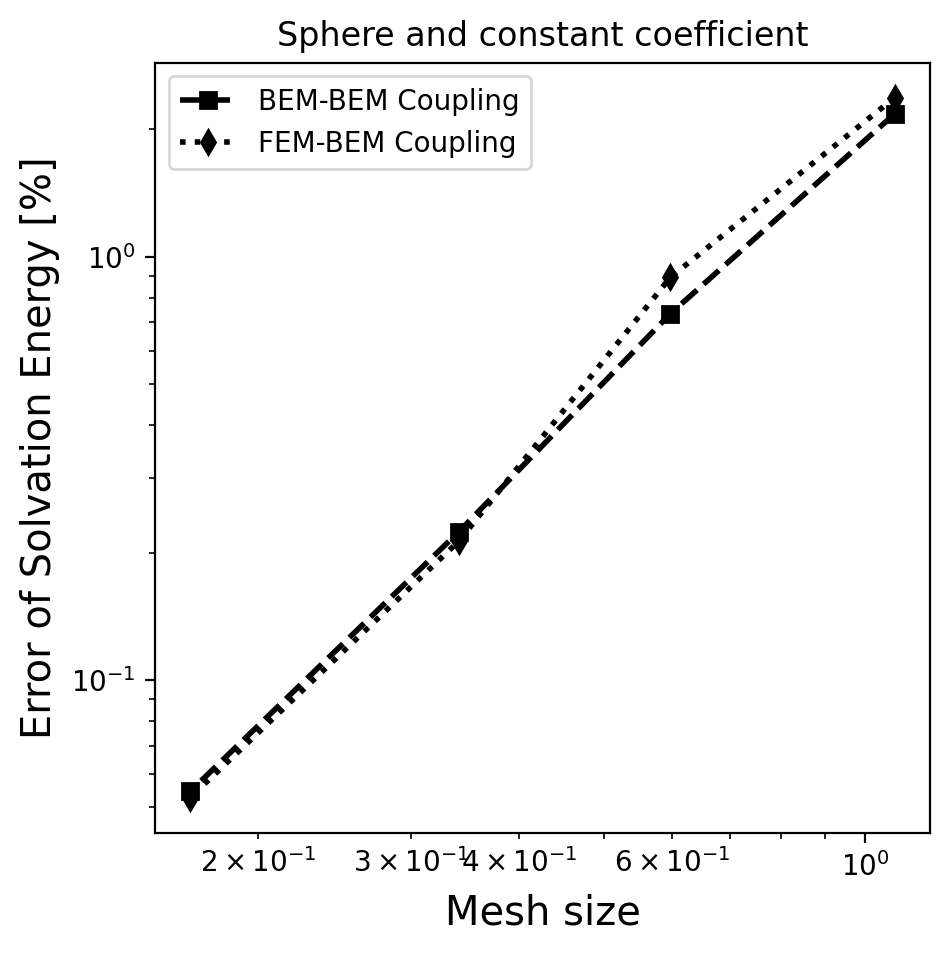
\includegraphics[width=0.6\linewidth]{DolfinX_Sphere_const_coeff_error.png}
  \caption{Error for the Kirkwood sphere.}
  \label{fig:error_sphere}
\end{figure}

\subsection*{\sffamily \large Performance with arginine}

As a more realistic test, we assessed the performance of the FEM-BEM coupling technique against a purely BEM implementation for arginine.
The structure of arginine taken from the protein data bank, and parameterized with the Amber\cite{ponder2003force} force field. 
We generated surface meshes containing 4.1, 6.7, 8.6, 17, and 24.5 vertices per \AA$^2$ with Nanoshaper.~\cite{decherchi2013general}
These densities correspond to a grid scale parameter in Nanoshaper equal to 1.6, 2.0, 2.4, 3.4, and 4.0, respectively, where the grid scale is the reciprocal of the average characteristic length of the triangles.
The surface meshes were inputs to our purely BEM solver and to create the FEM mesh with pyGAMer,~\cite{lee2020open} which invoked TetGen\cite{hang2015tetgen} with a quality parameter (radius-edge ratio) of 1.0.

The solvation energy computed with the two schemes is presented by Figure \ref{fig:arg_constant_energy}, which, as expected, converges to a similar answer as the mesh is refined.
Then, Figure \ref{fig:arg2_constant_time_iter} compares the iteration count and time-to-solution. The left plot shows that using only BEM outperforms the coupled FEM-BEM approach in terms of iterations count. However, if we look at the total time that solvers take to obtain the solution, we can see the advantage of using the FEM-BEM coupling. The higher computational cost is caused by the need of using a hypersingular operator in the BEM formulation.


\begin{figure}
\centering
   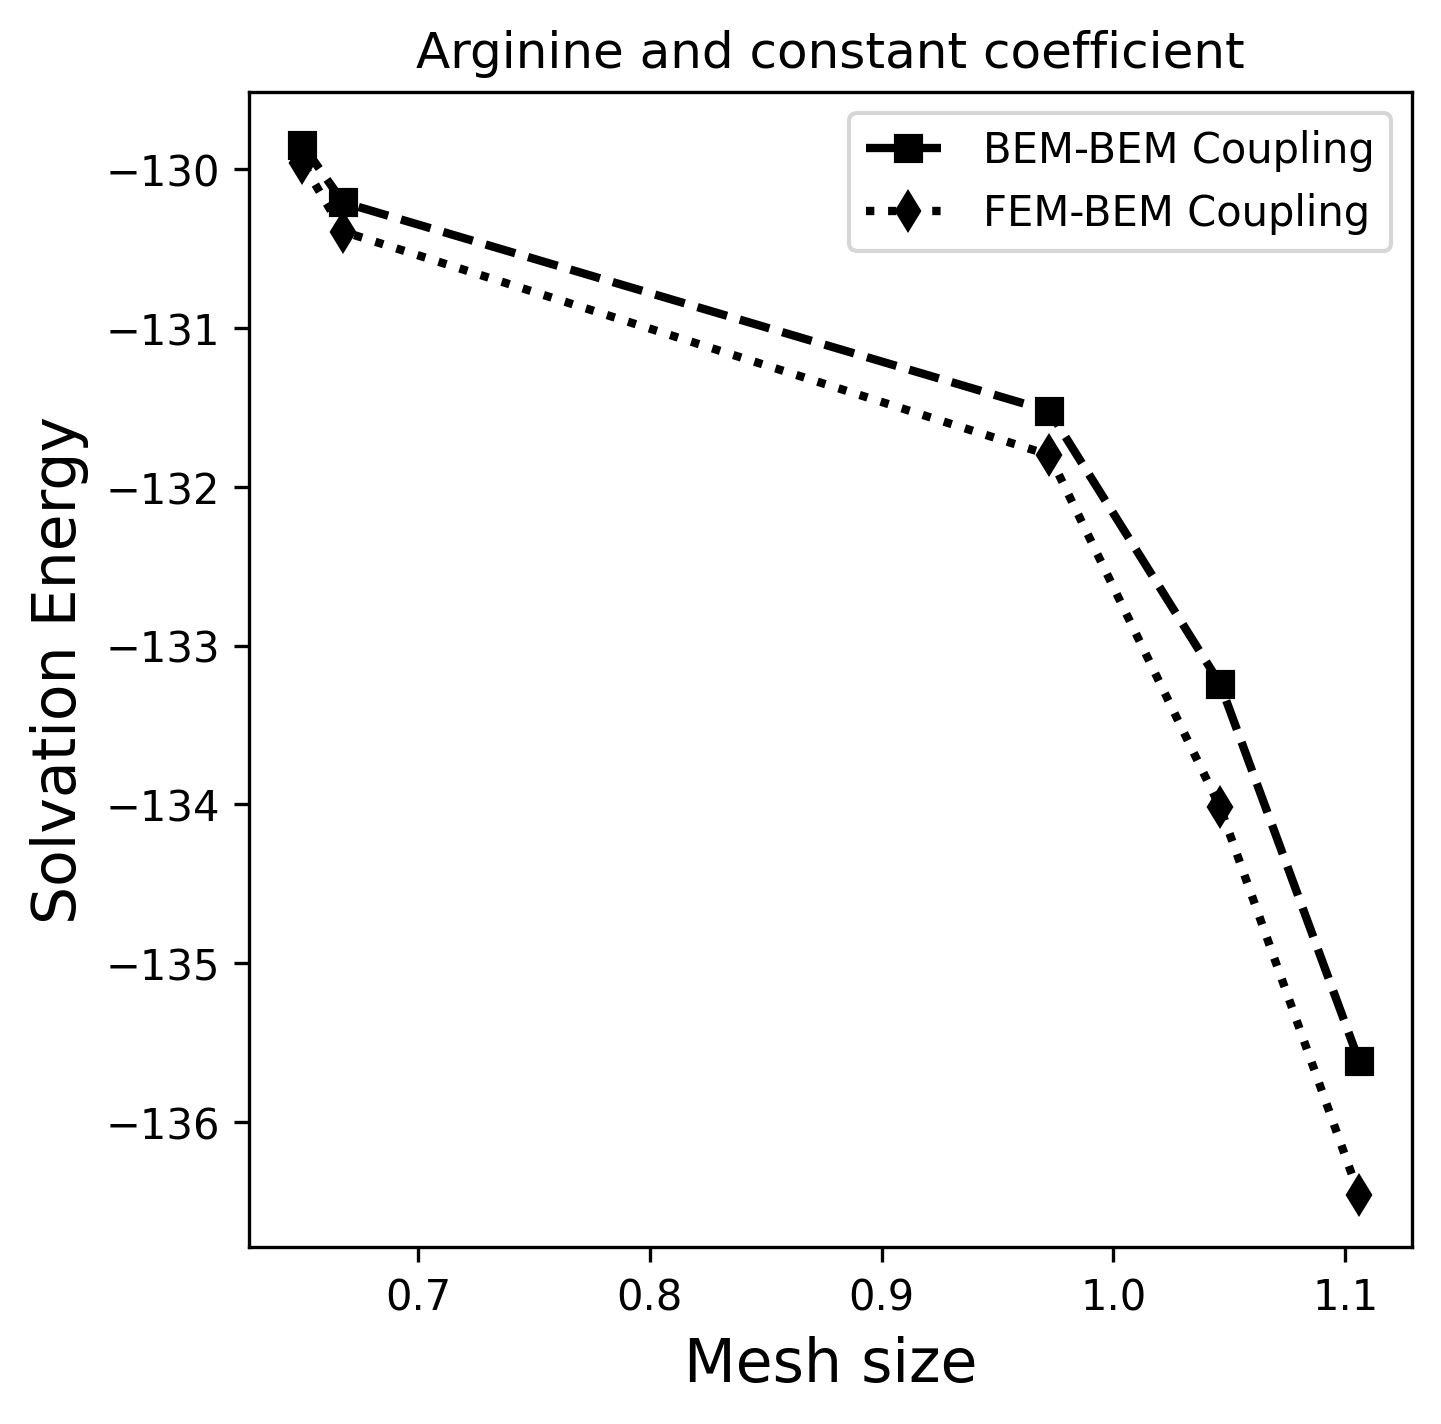
\includegraphics[width=0.47\linewidth]{DolfinX_Arginine2_const_coeff_error.png}
%   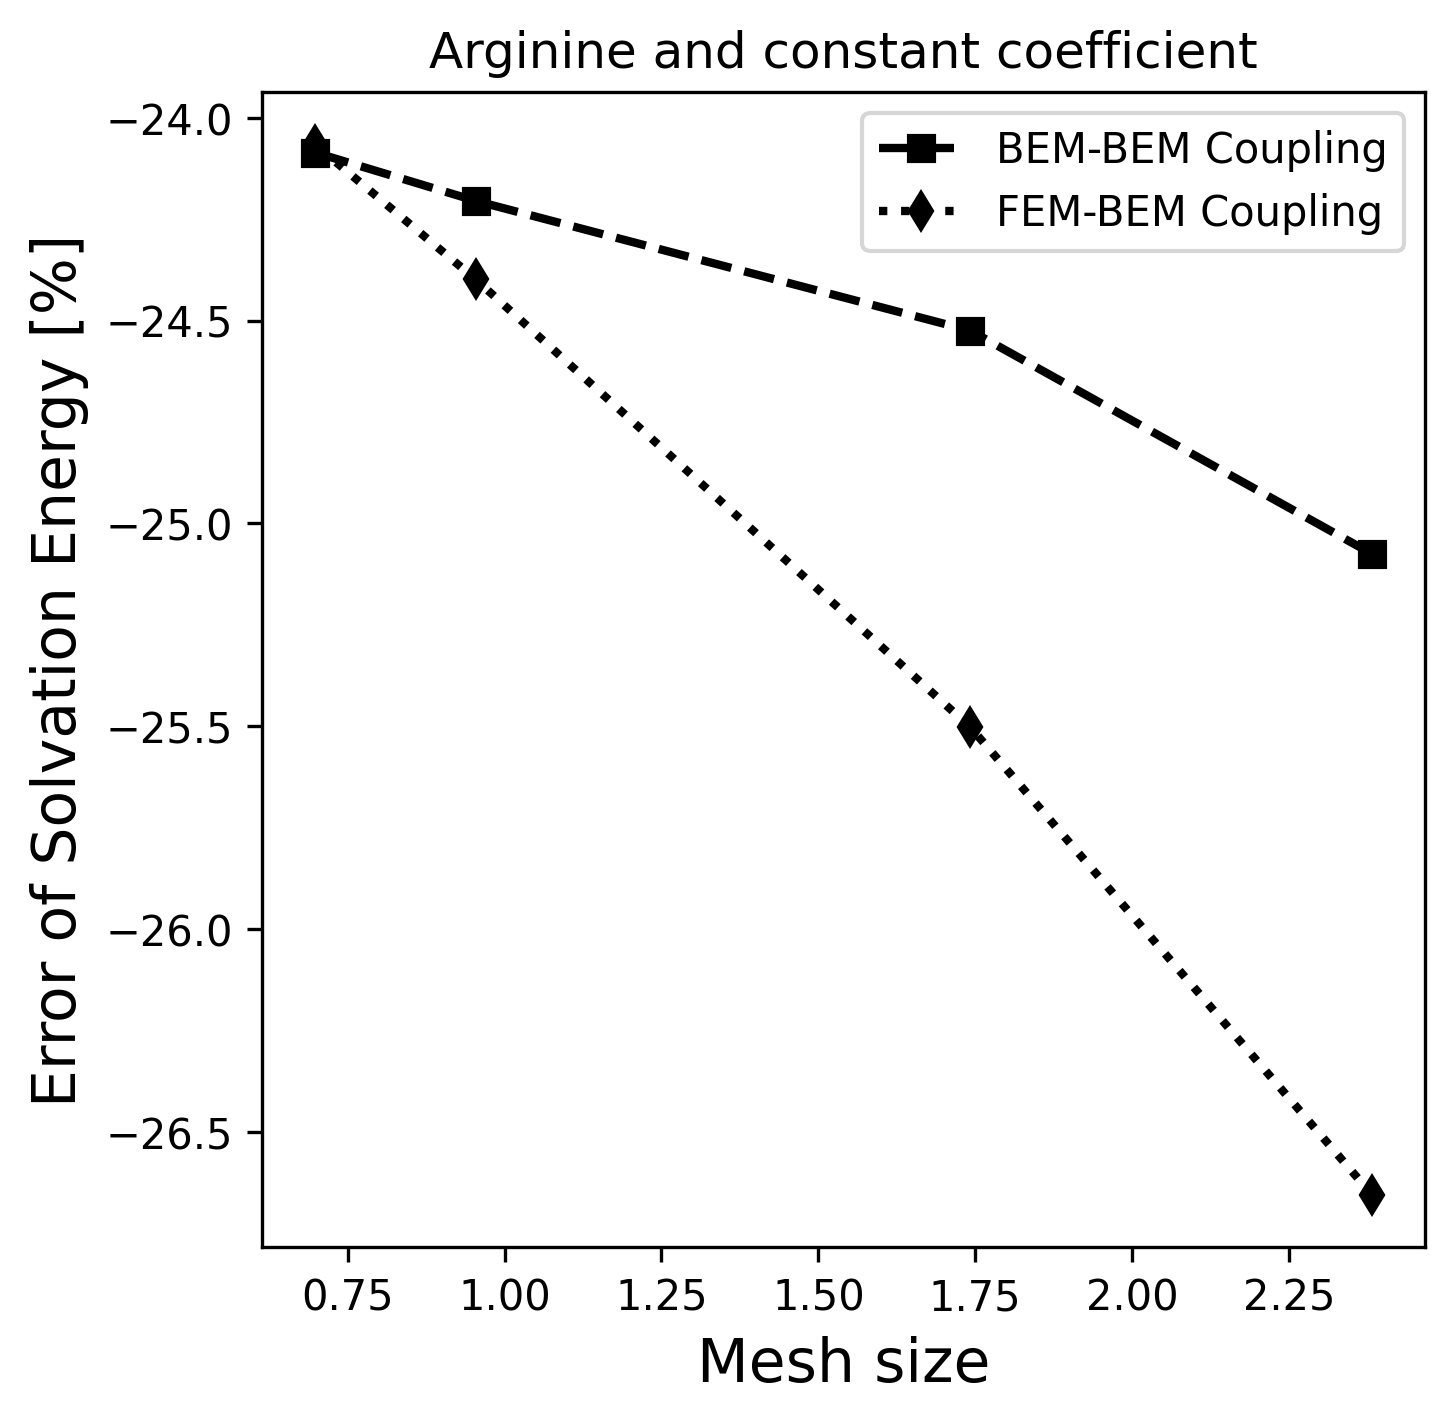
\includegraphics[width=0.47\linewidth]{DolfinX_Arginine_const_coeff_error_11.png}
\caption{Solvation energy for arginine with a constant permittivity. %(left - Arginine2 and right - Arginine)
%maybe we could also add a "error" wrt extrapolation, or a plot with energy for each mesh?
}
\label{fig:arg_constant_energy}
\end{figure}

\begin{figure}
\centering
   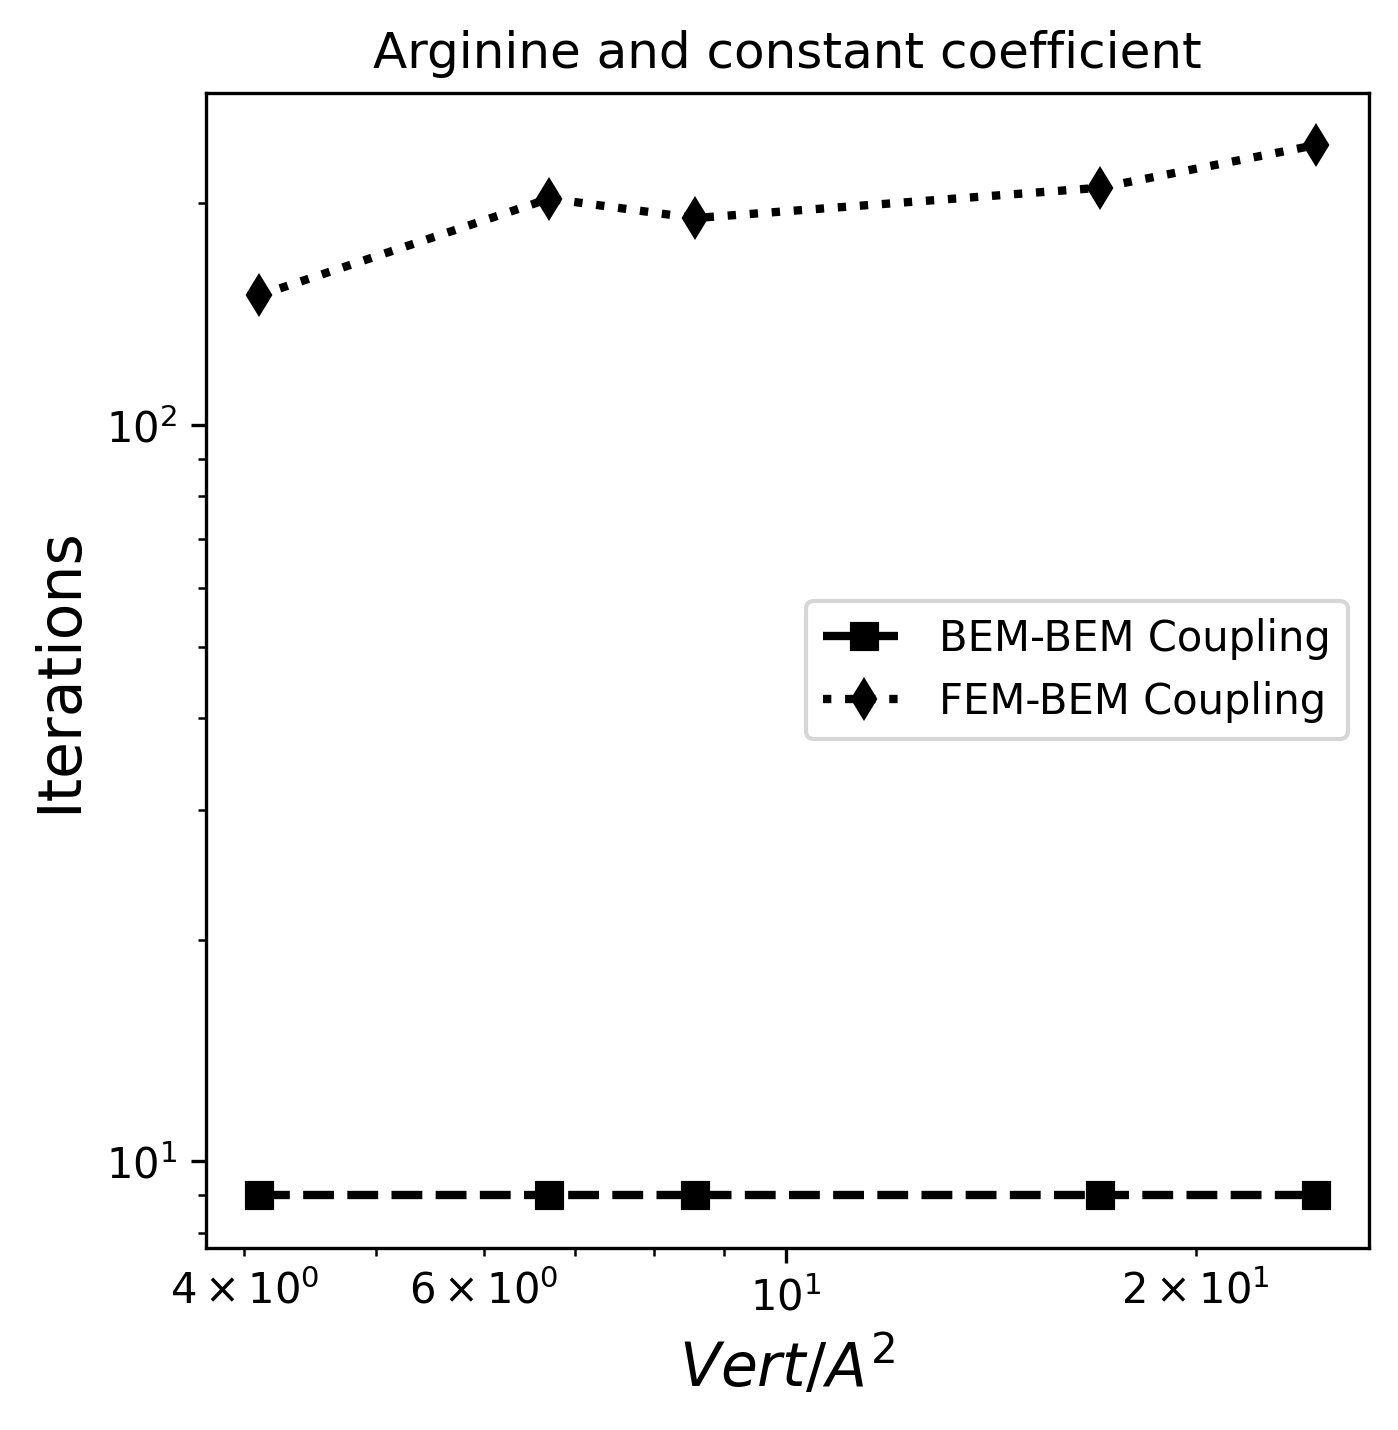
\includegraphics[width=0.45\linewidth]{DolfinX_Arginine2_const_coeff_iter.png}
%  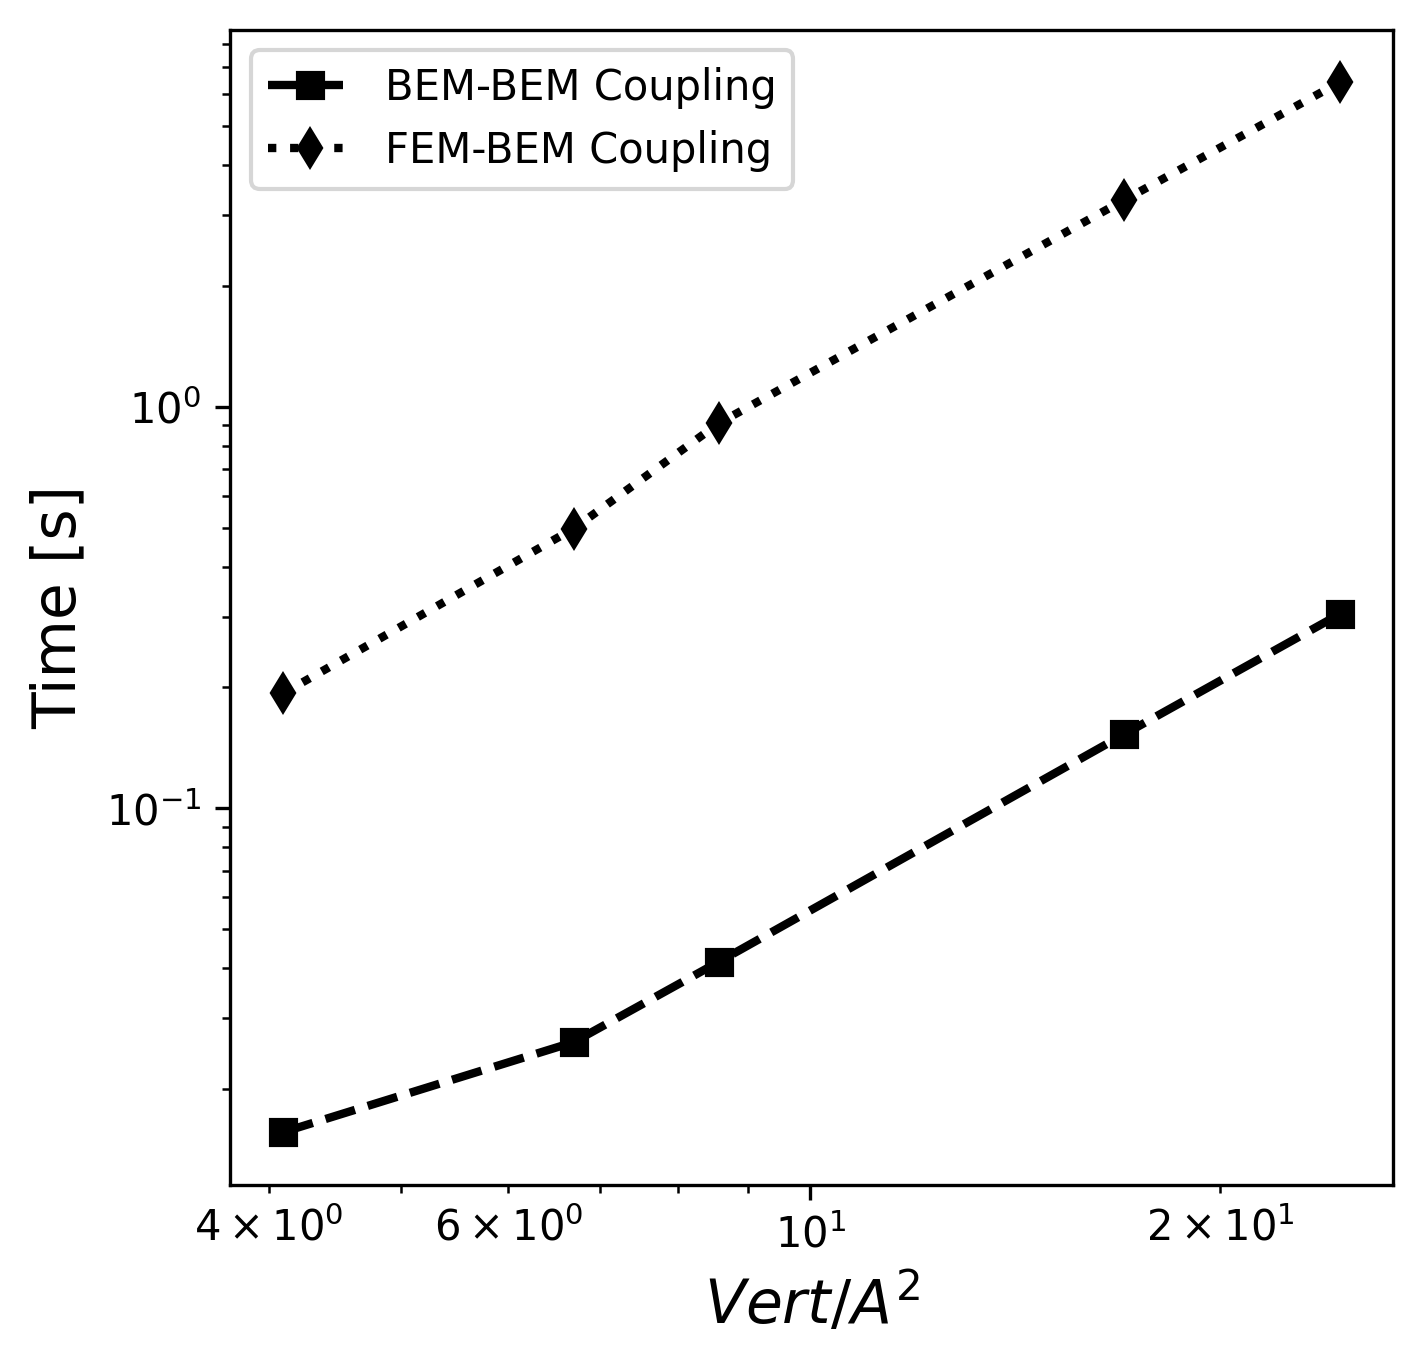
\includegraphics[width=0.45\linewidth]{DolfinX_Arginine2_const_coeff_time.png}
%  \includegraphics[width=0.45\linewidth]{DolfinX_Arginine2_const_coeff_setup_time.png}
  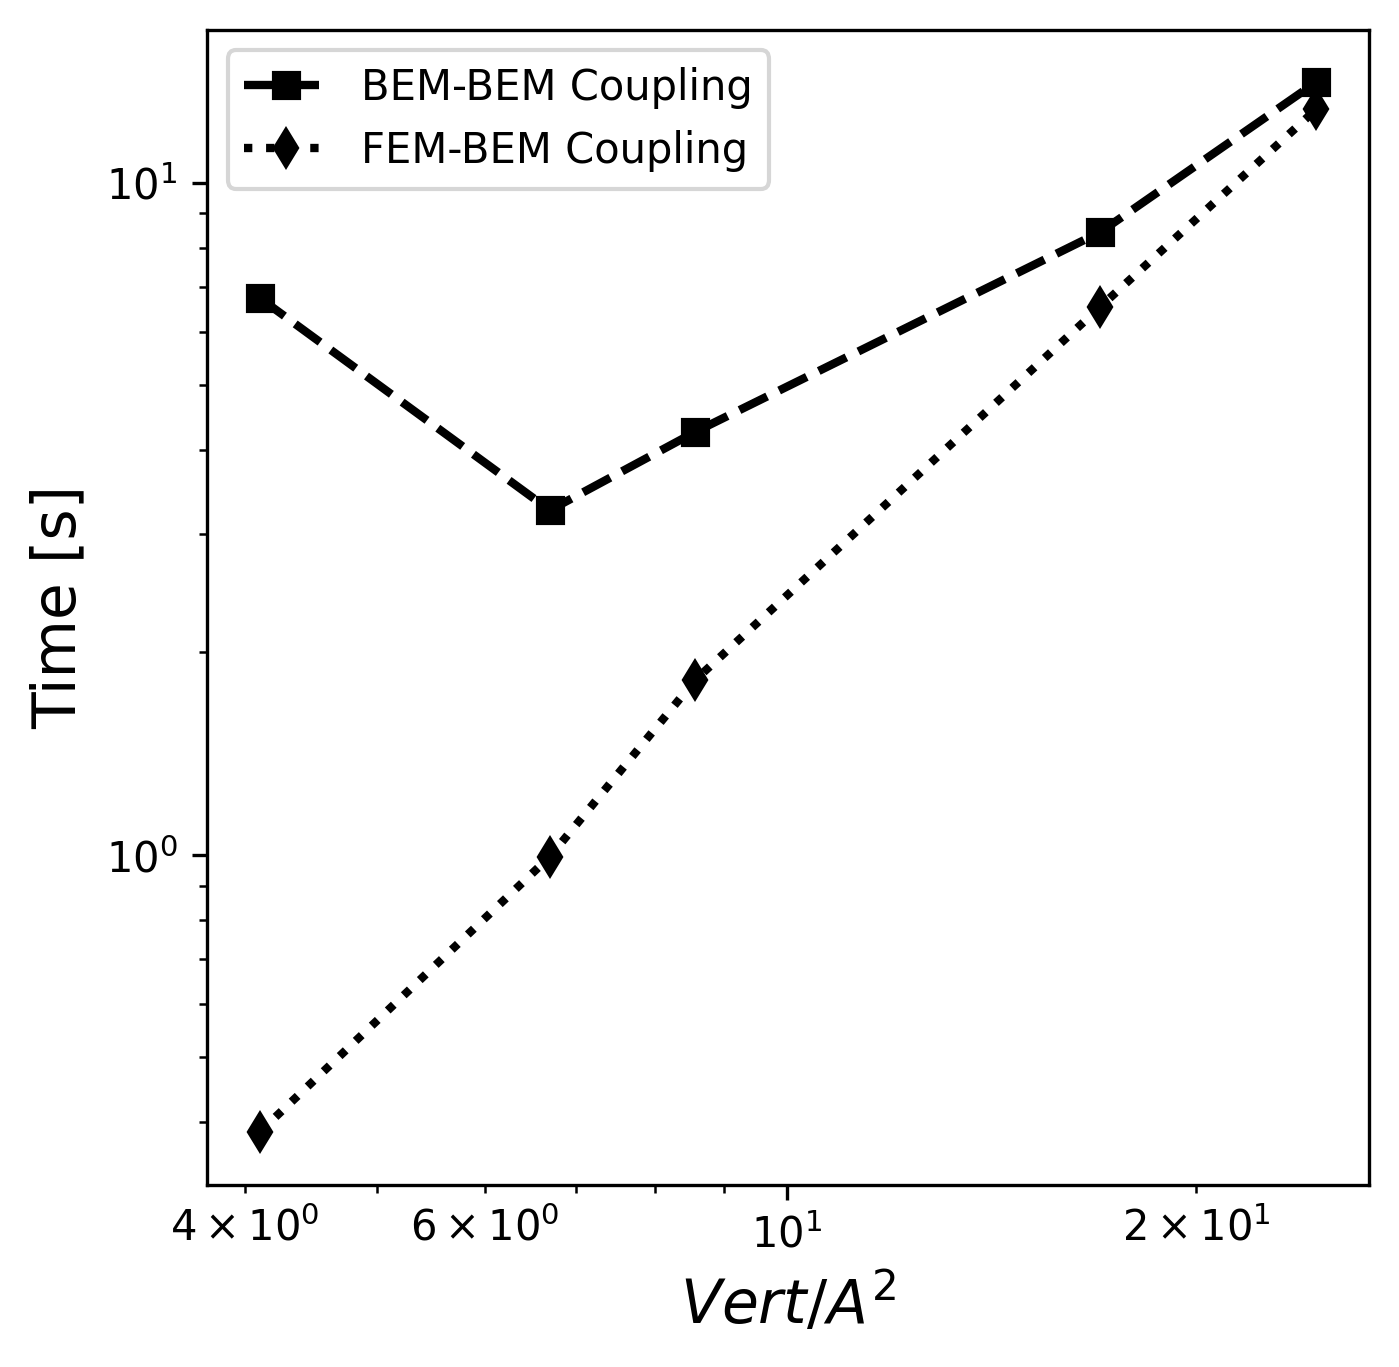
\includegraphics[width=0.45\linewidth]{DolfinX_Arginine2_const_coeff_total_time.png}
%   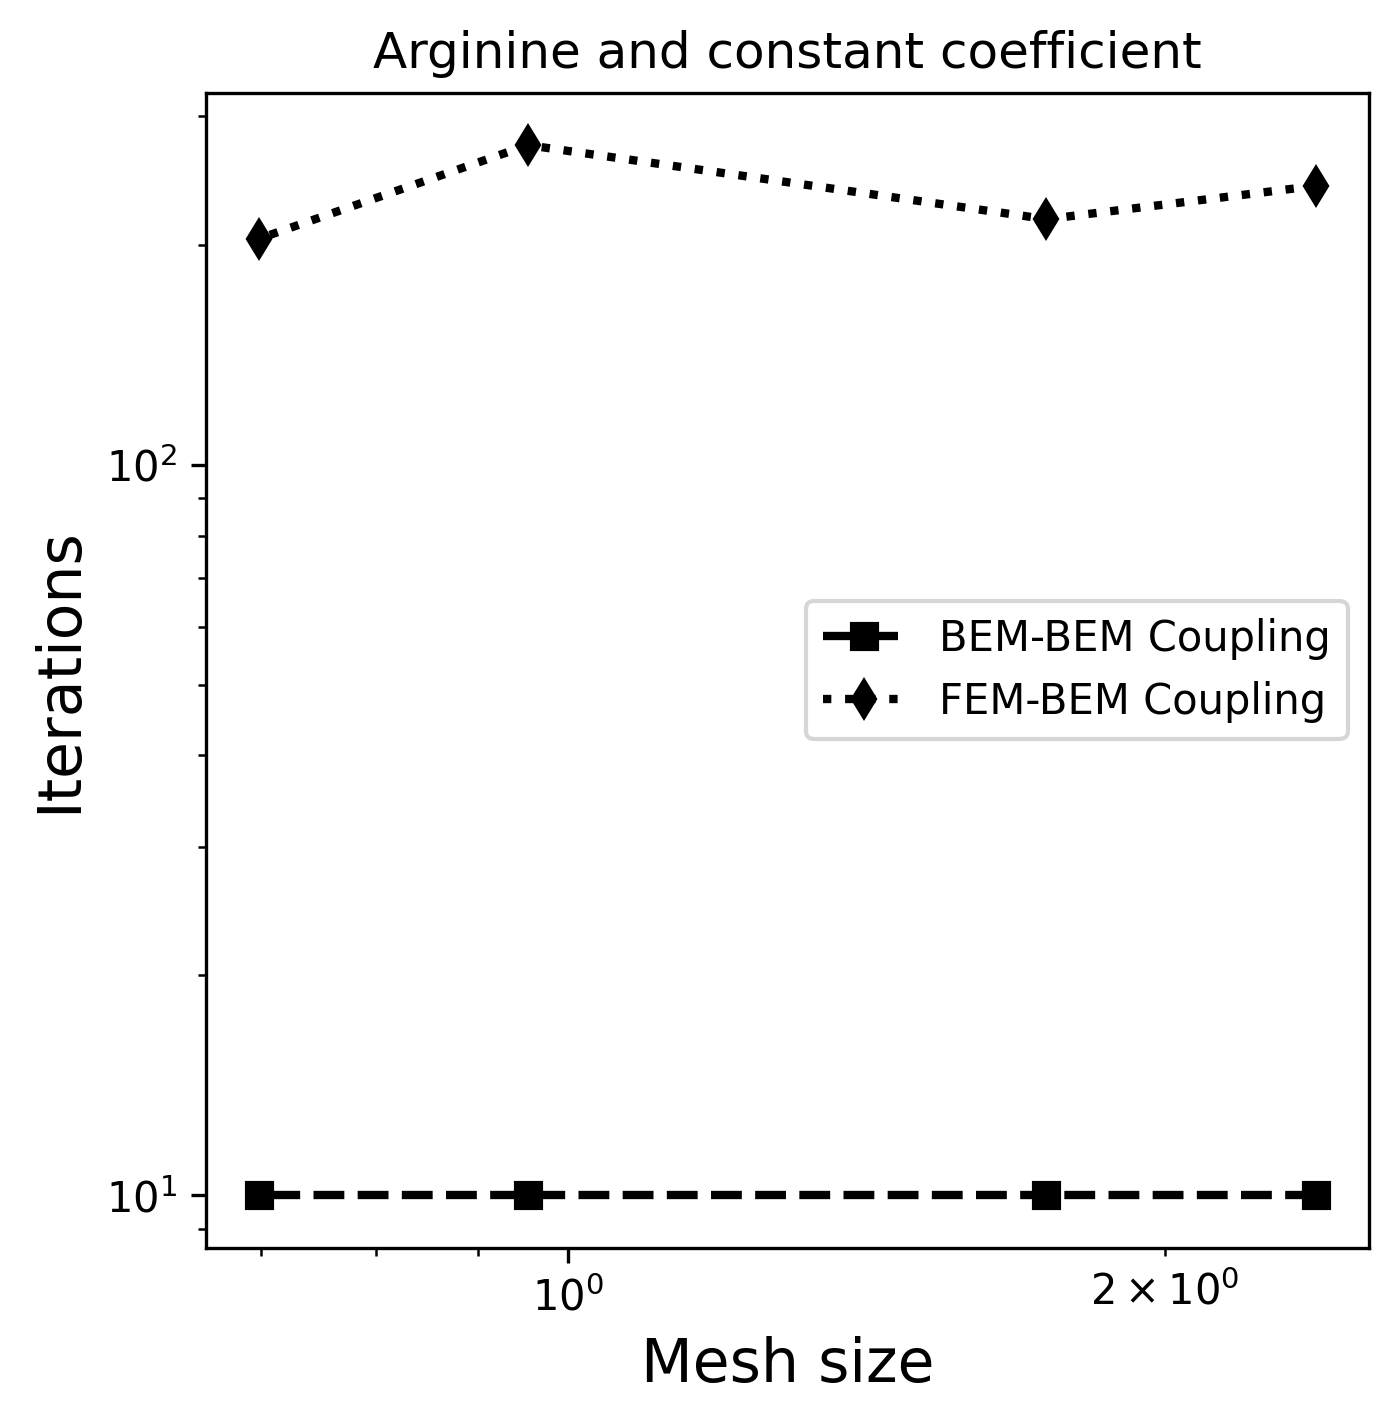
\includegraphics[width=0.45\linewidth]{DolfinX_Arginine_const_coeff_iter_11.png}
%%  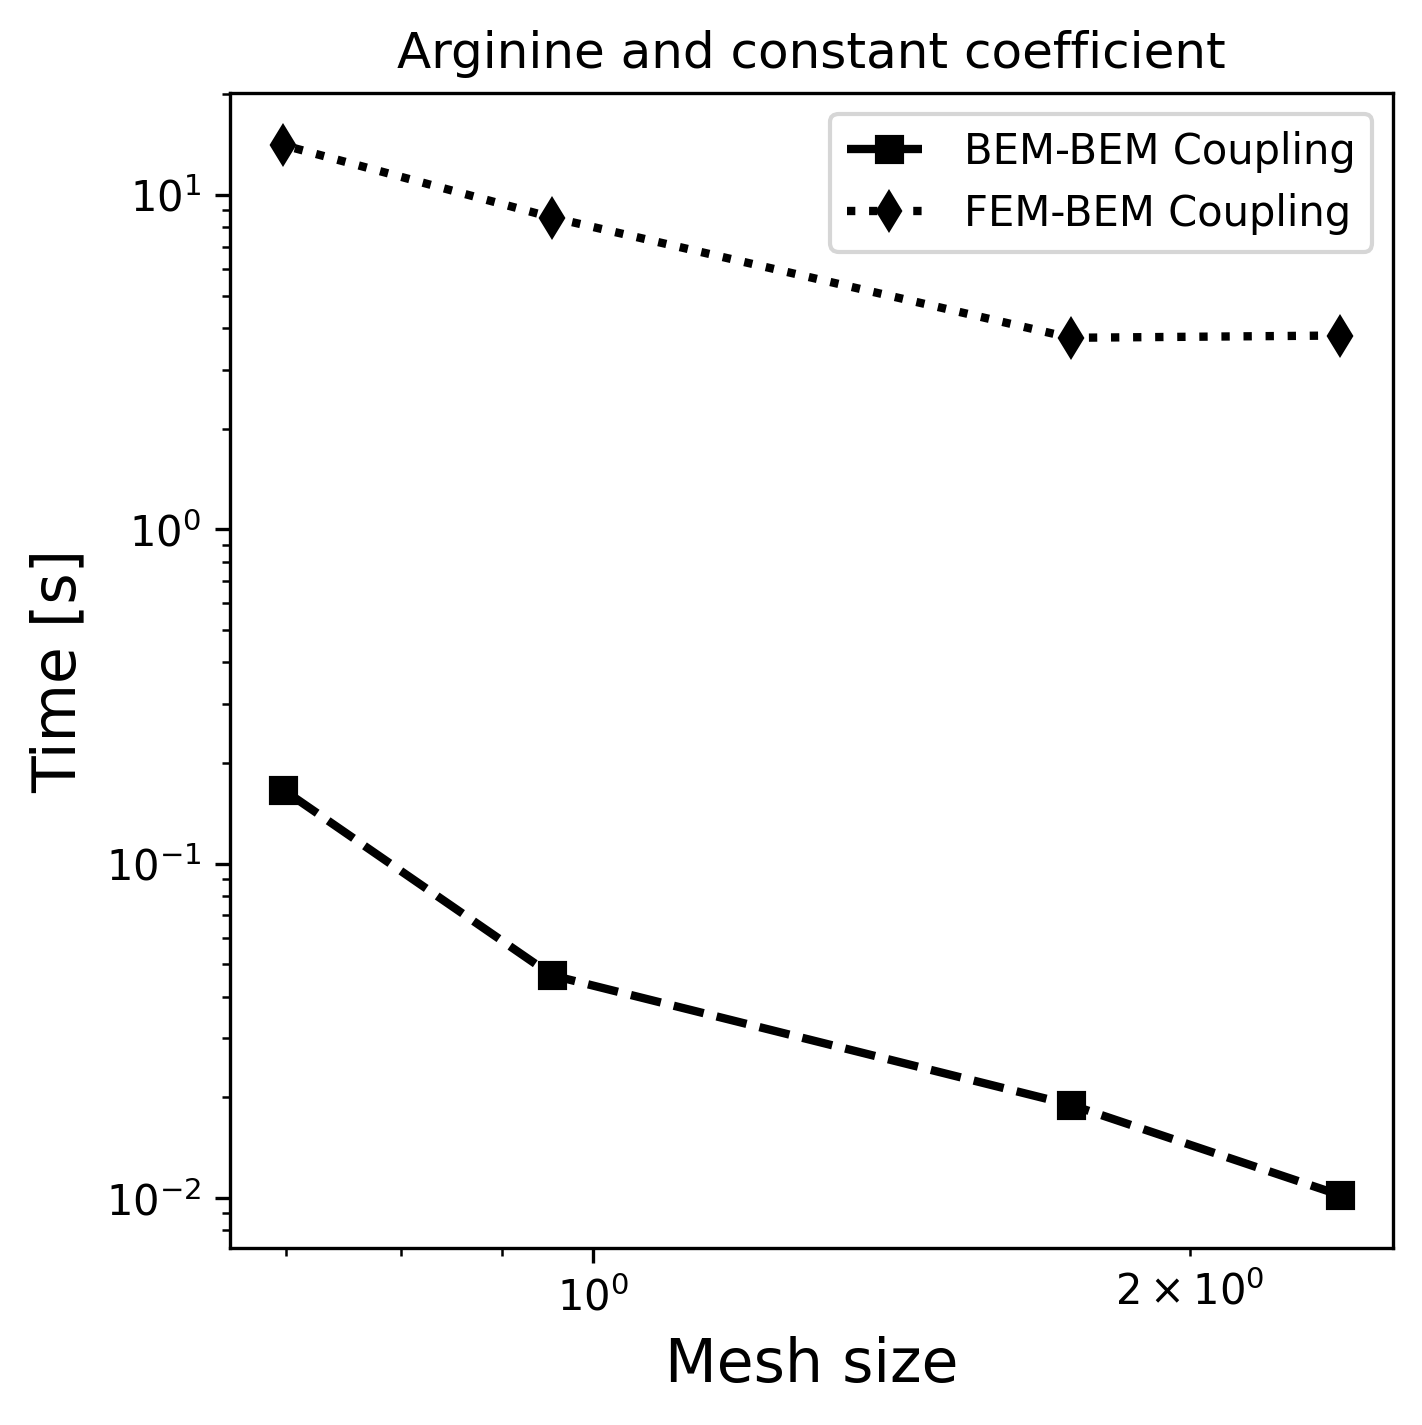
\includegraphics[width=0.45\linewidth]{DolfinX_Arginine_const_coeff_time_11.png}
%%  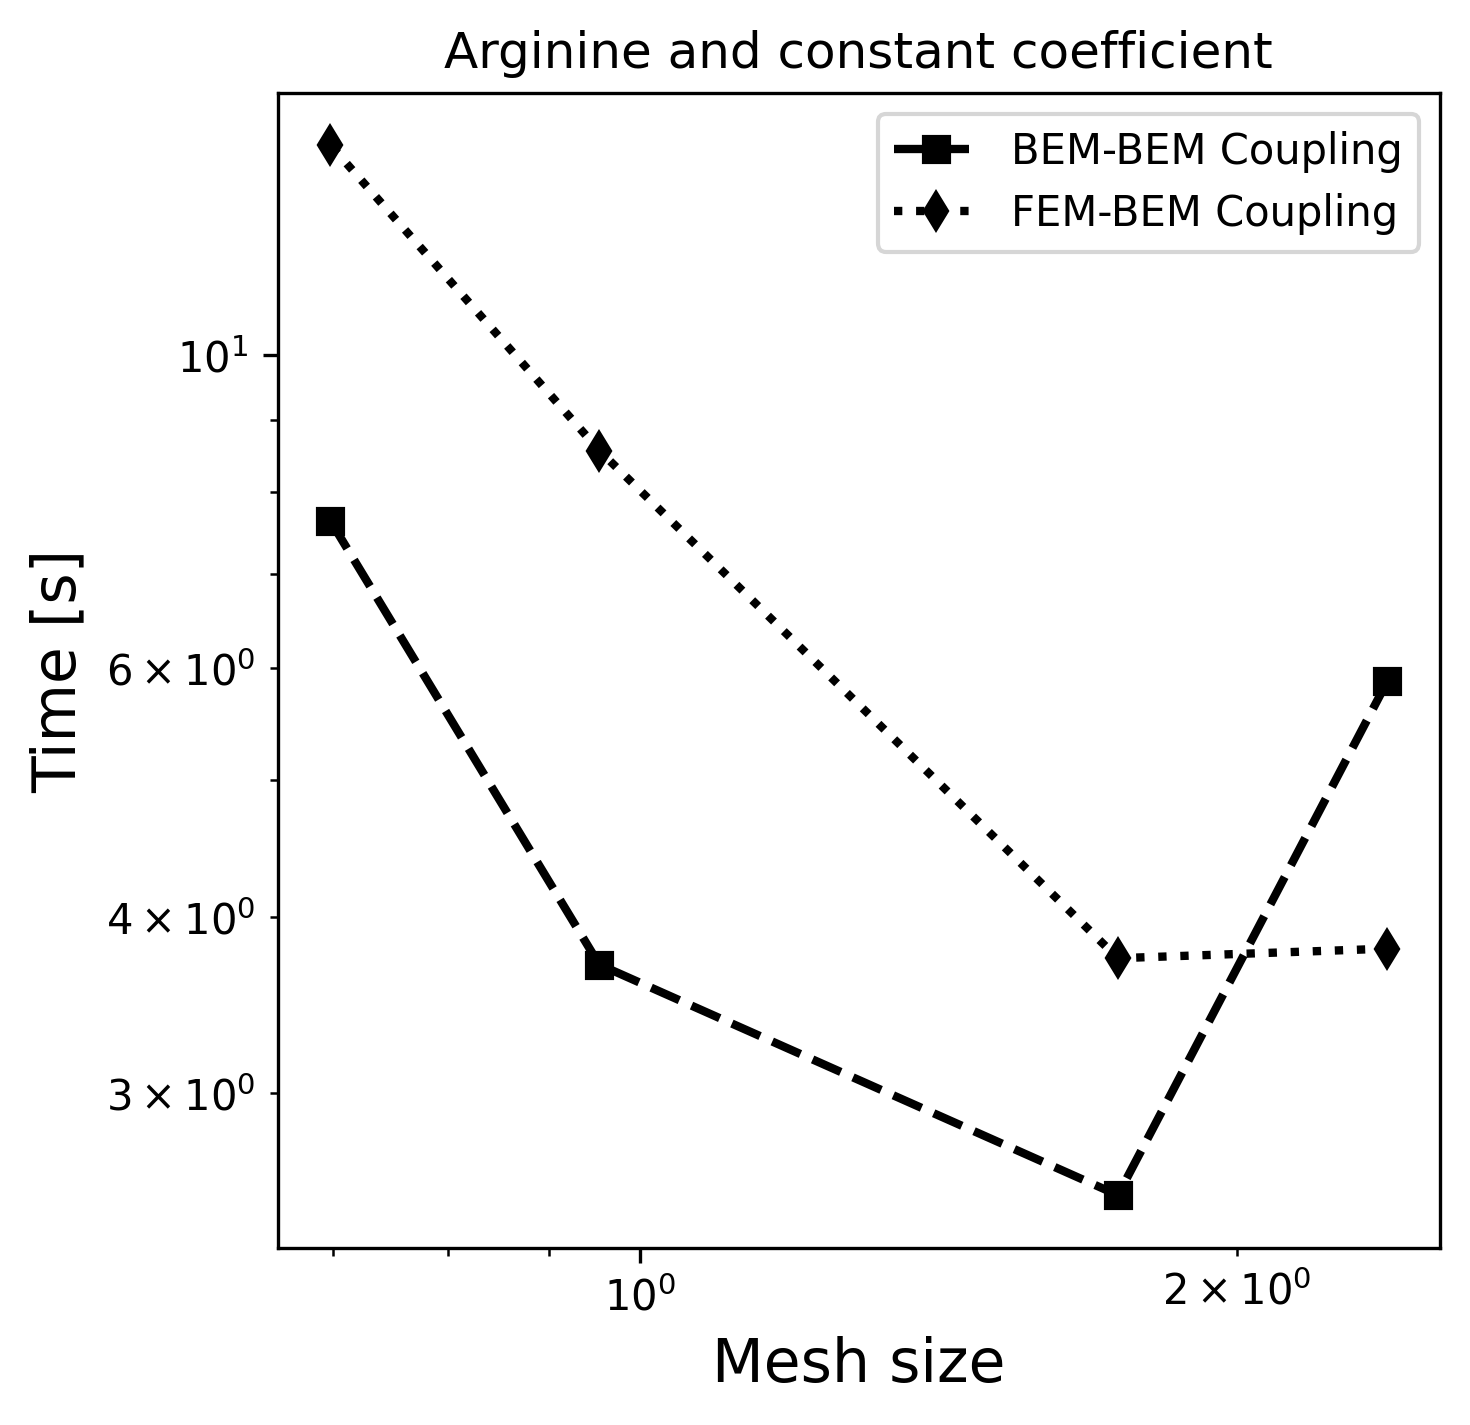
\includegraphics[width=0.45\linewidth]{DolfinX_Arginine_const_coeff_setup_time_11.png}
%  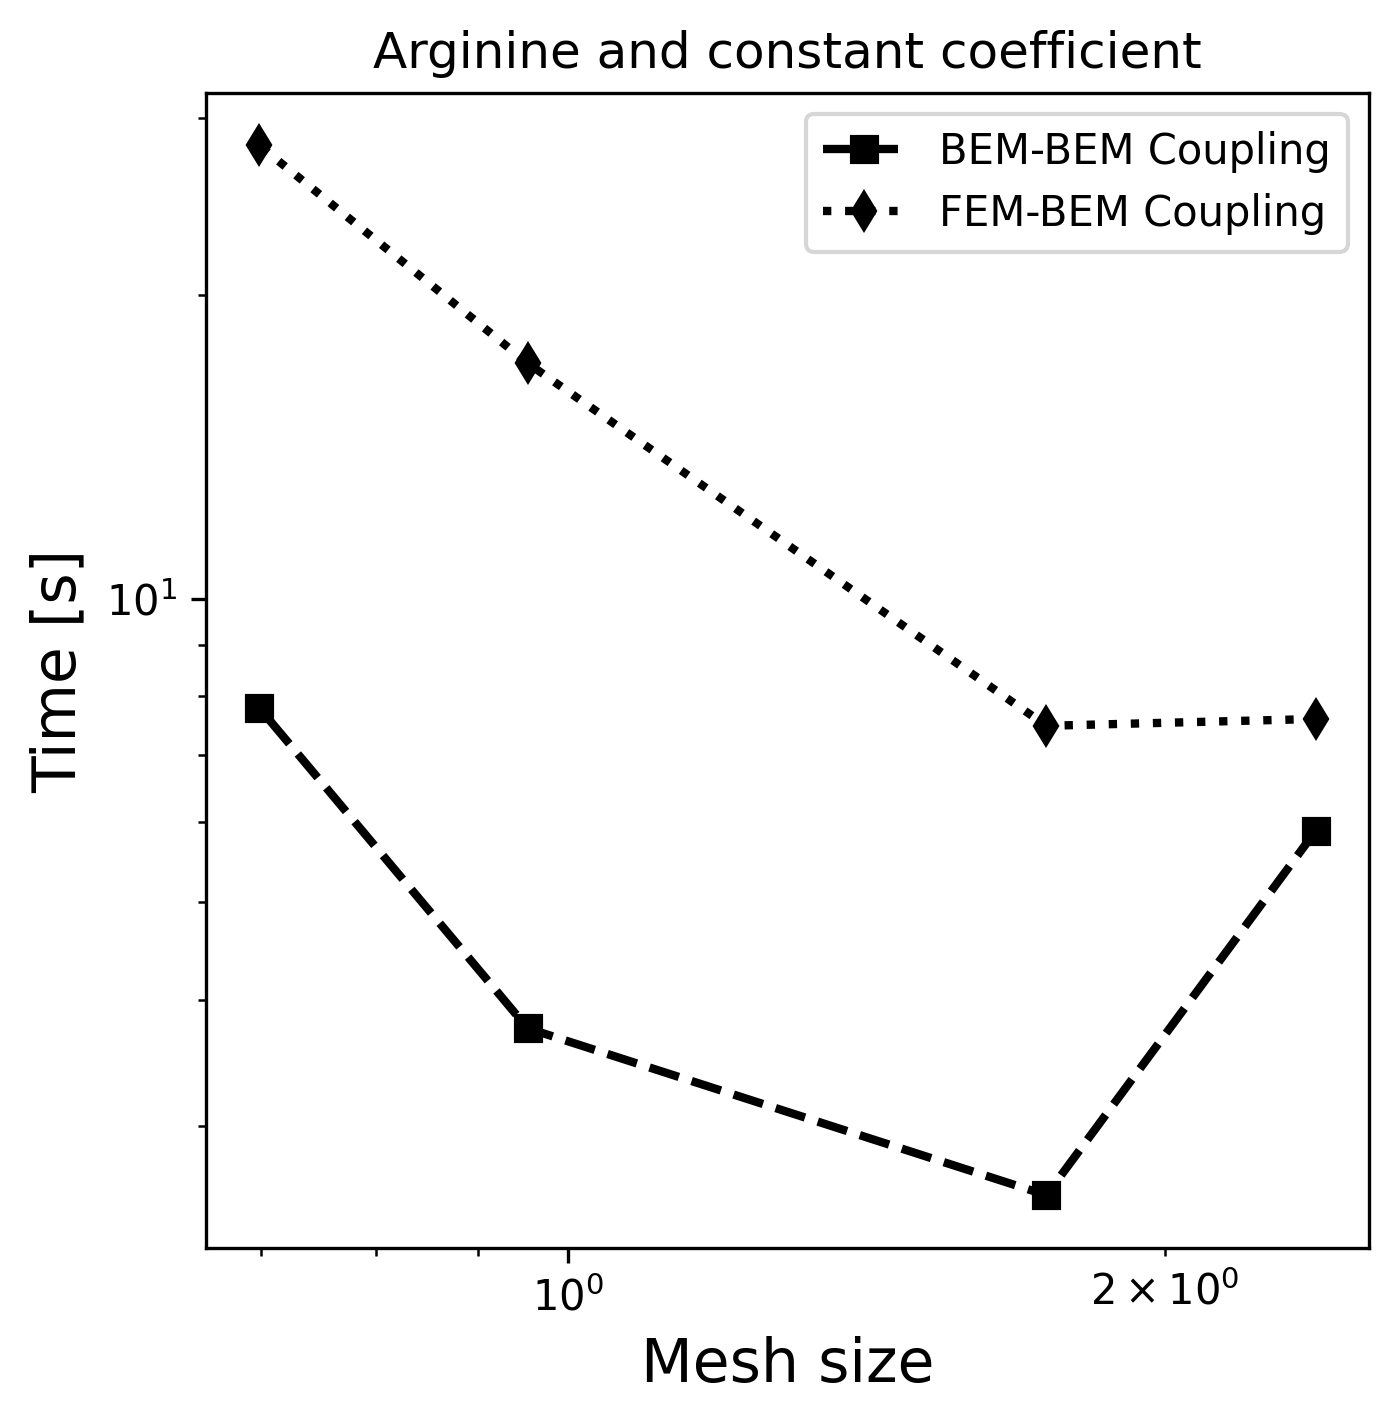
\includegraphics[width=0.45\linewidth]{DolfinX_Arginine_const_coeff_total_time_11.png}
  \caption{Iteration count (left) and time-to-solution (right) for Arginine with a constant permittivity. %(left: Online time taken to solve systems, right: Offline time taken to set up systems). 
%NOTE: x axis differ between top and bottom. Also, should we include preconditioned vs non preconditioned? We could easily precondition BEM-BEM too.  %(1) fix title, (2) can we put them in a single plot, (3) 
%maybe we could also add a "error" wrt extrapolation, or a plot with energy for each mesh?
}
\label{fig:arg2_constant_time_iter}
\end{figure}

%\begin{figure}
%\centering
%%   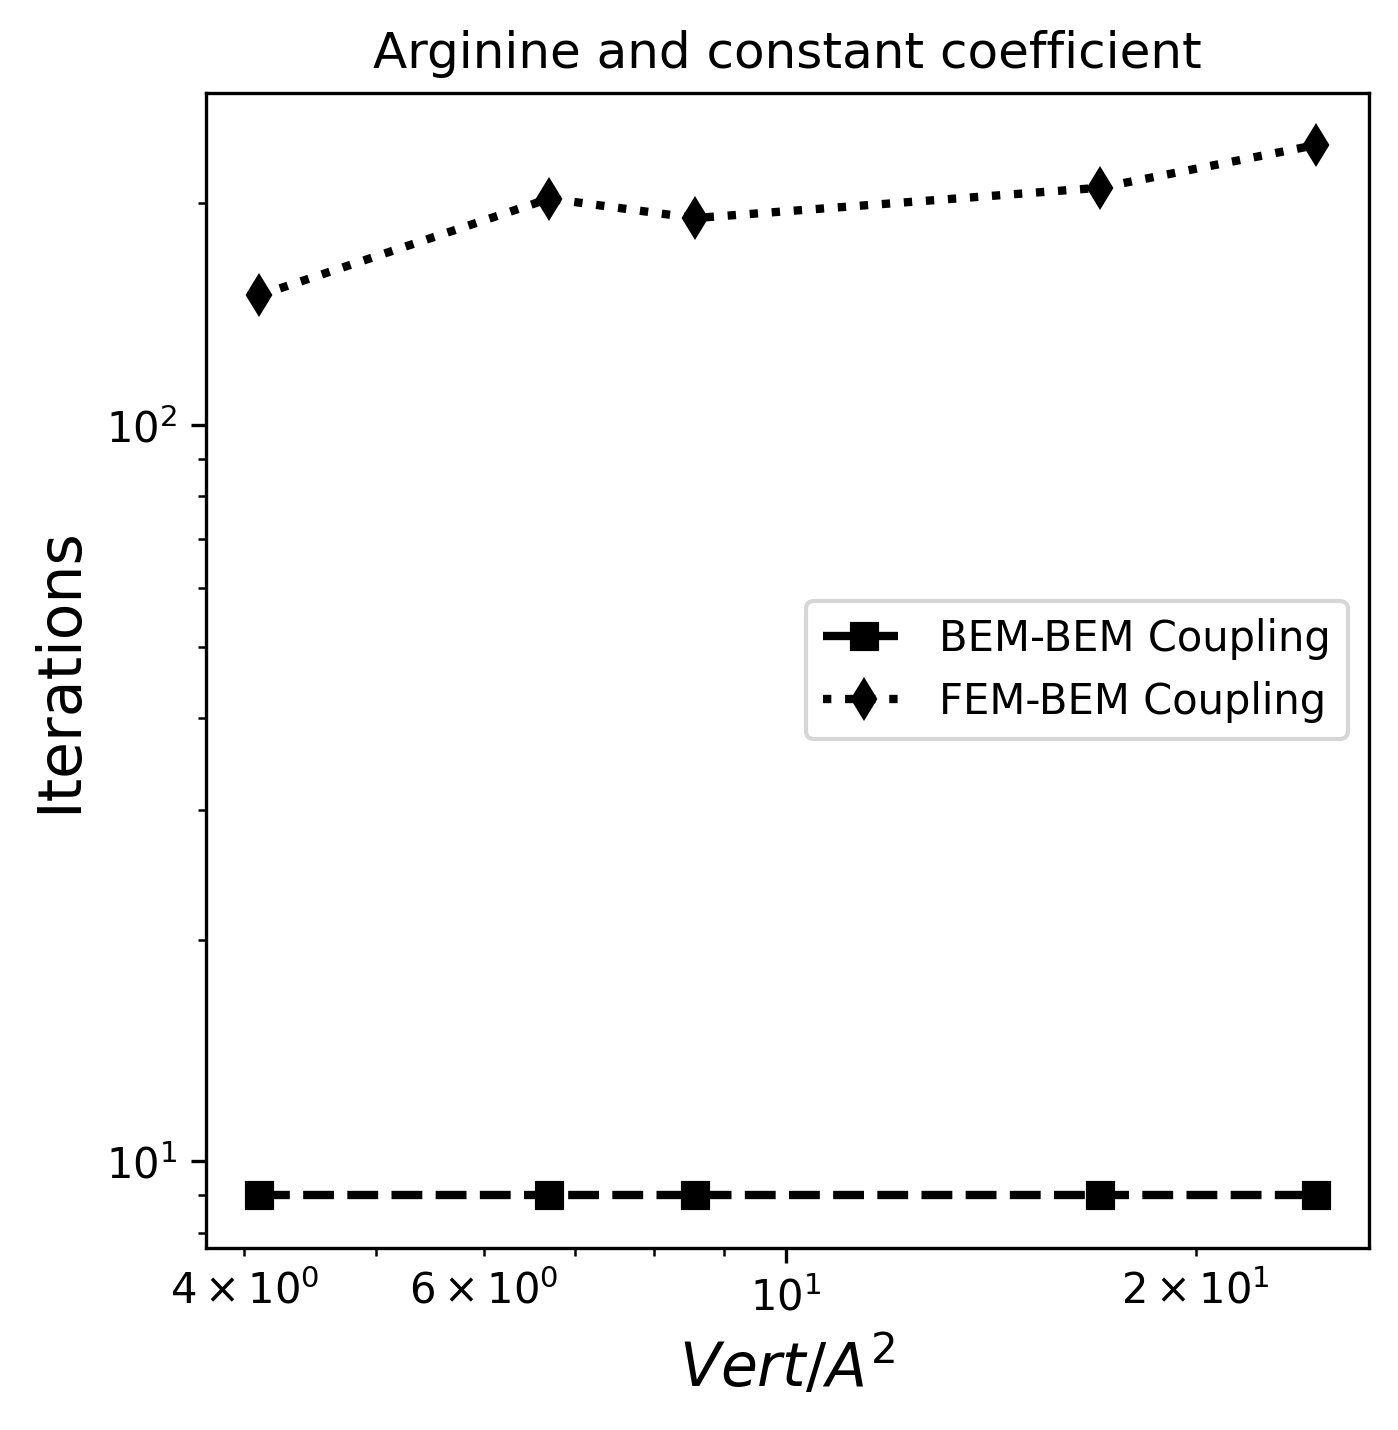
\includegraphics[width=0.45\linewidth]{DolfinX_Arginine2_const_coeff_iter.png}
%%%  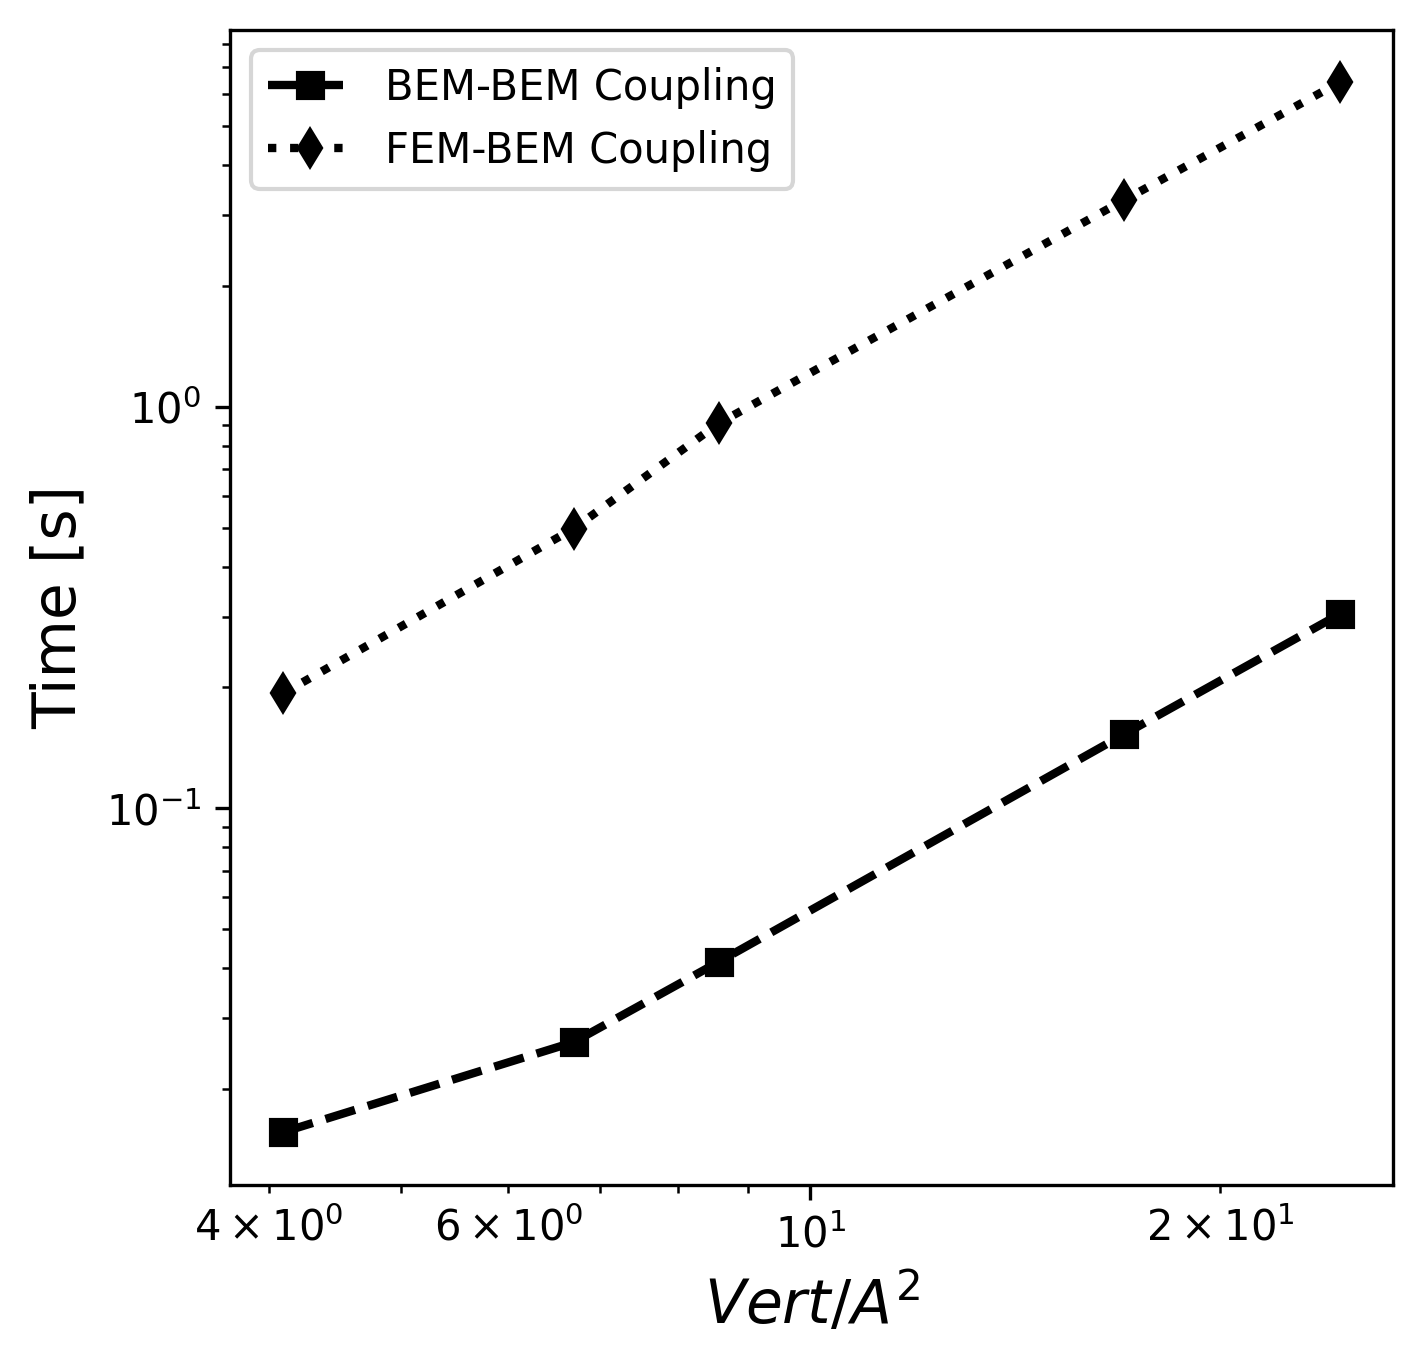
\includegraphics[width=0.45\linewidth]{DolfinX_Arginine2_const_coeff_time.png}
%%%  \includegraphics[width=0.45\linewidth]{DolfinX_Arginine2_const_coeff_setup_time.png}
%%  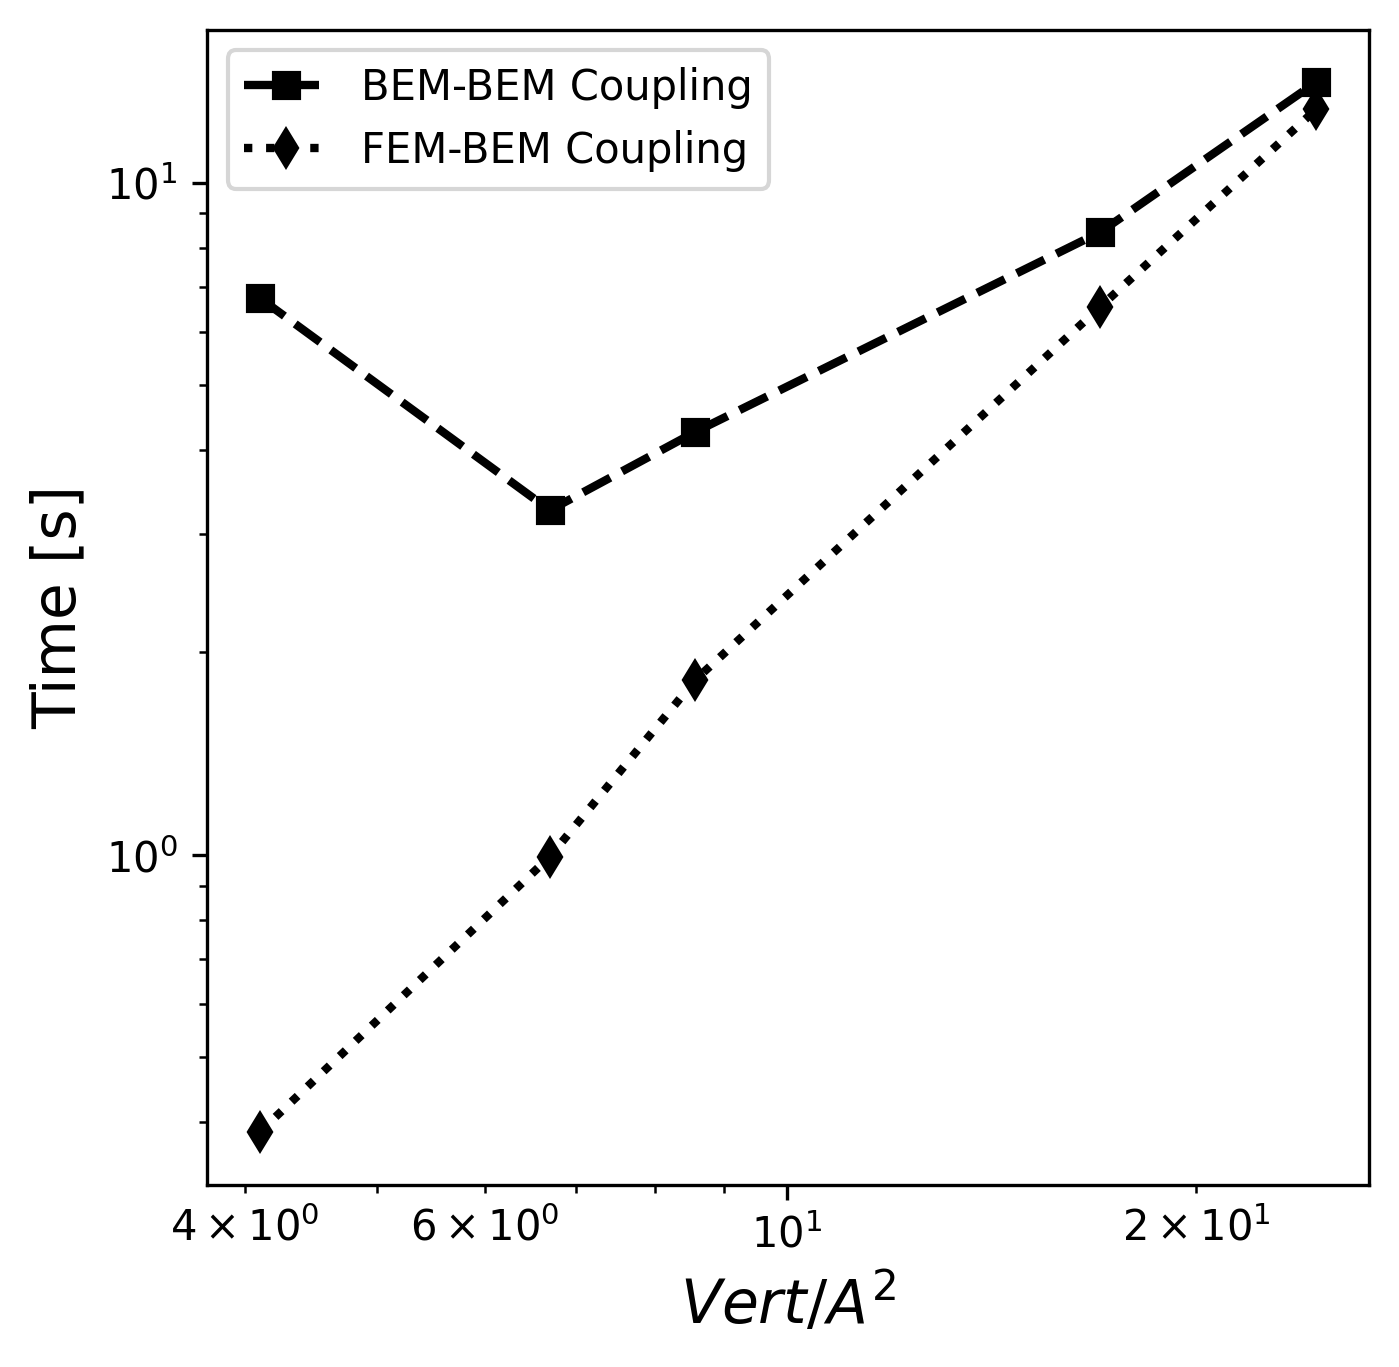
\includegraphics[width=0.45\linewidth]{DolfinX_Arginine2_const_coeff_total_time.png}
%   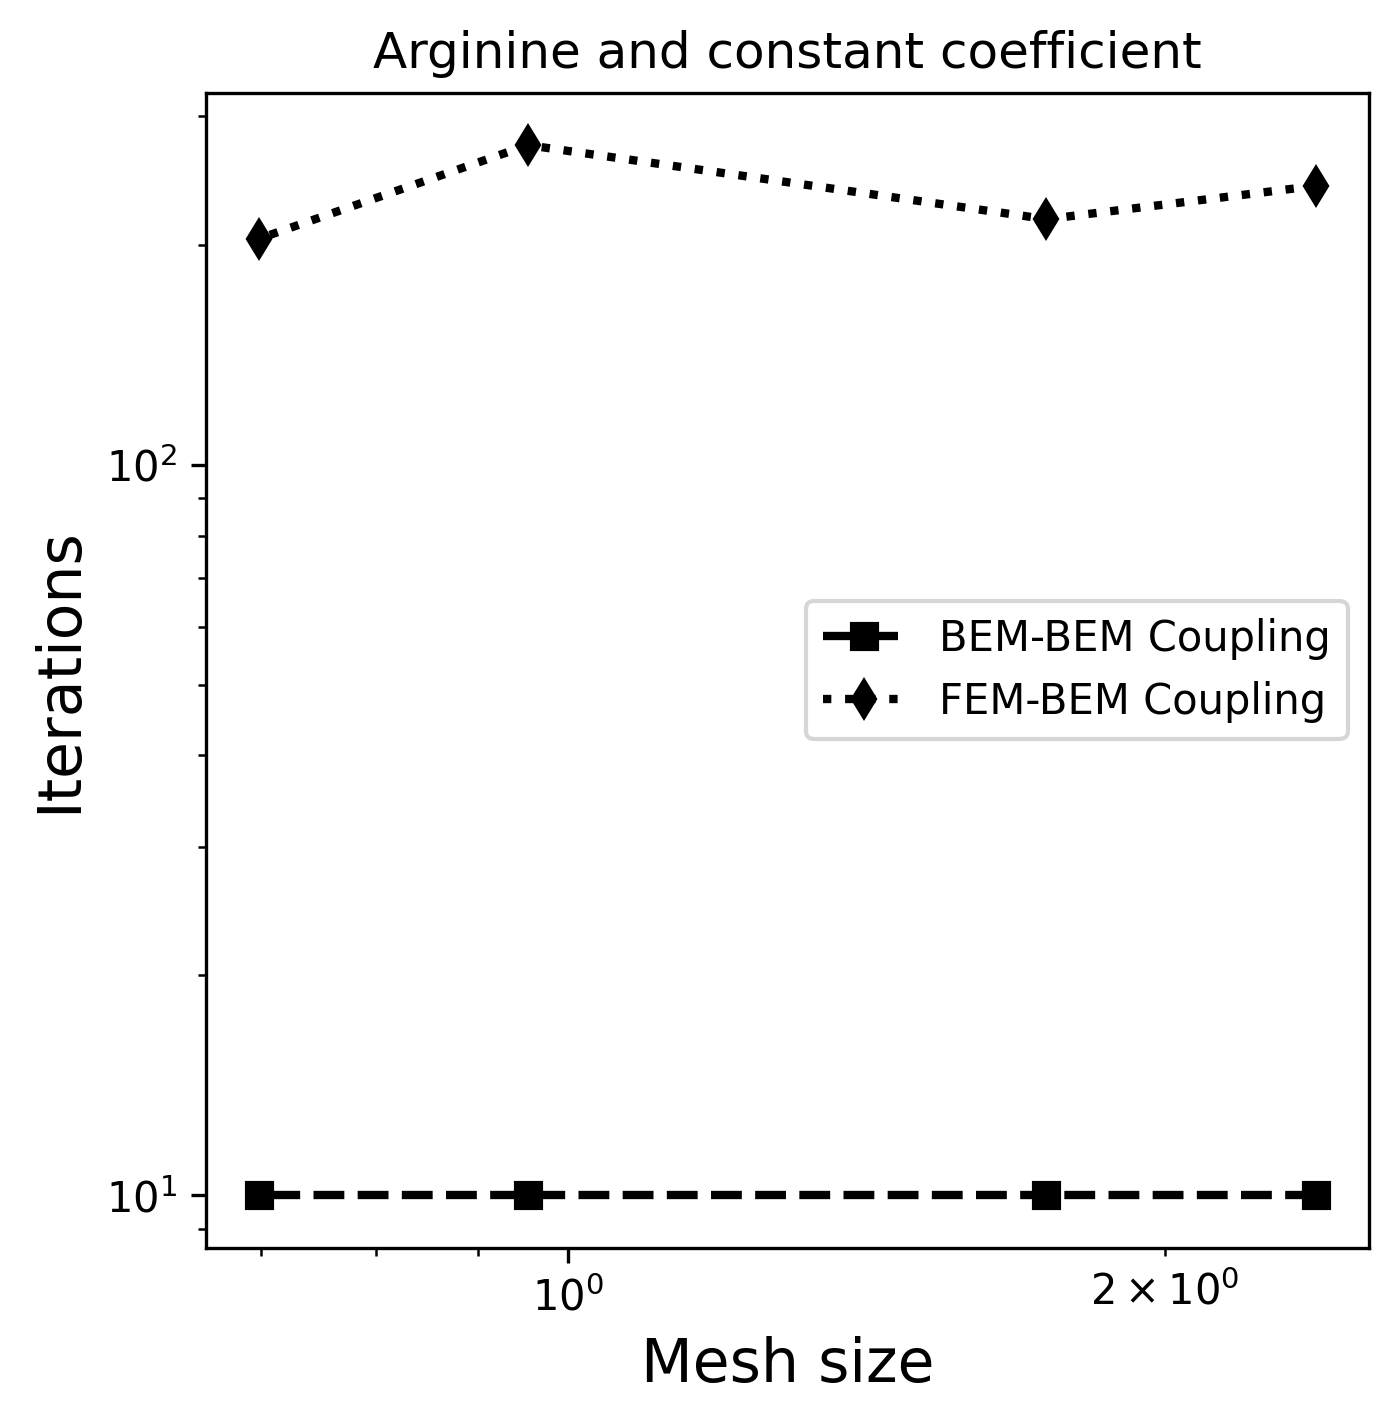
\includegraphics[width=0.45\linewidth]{DolfinX_Arginine_const_coeff_iter_11.png}
%%  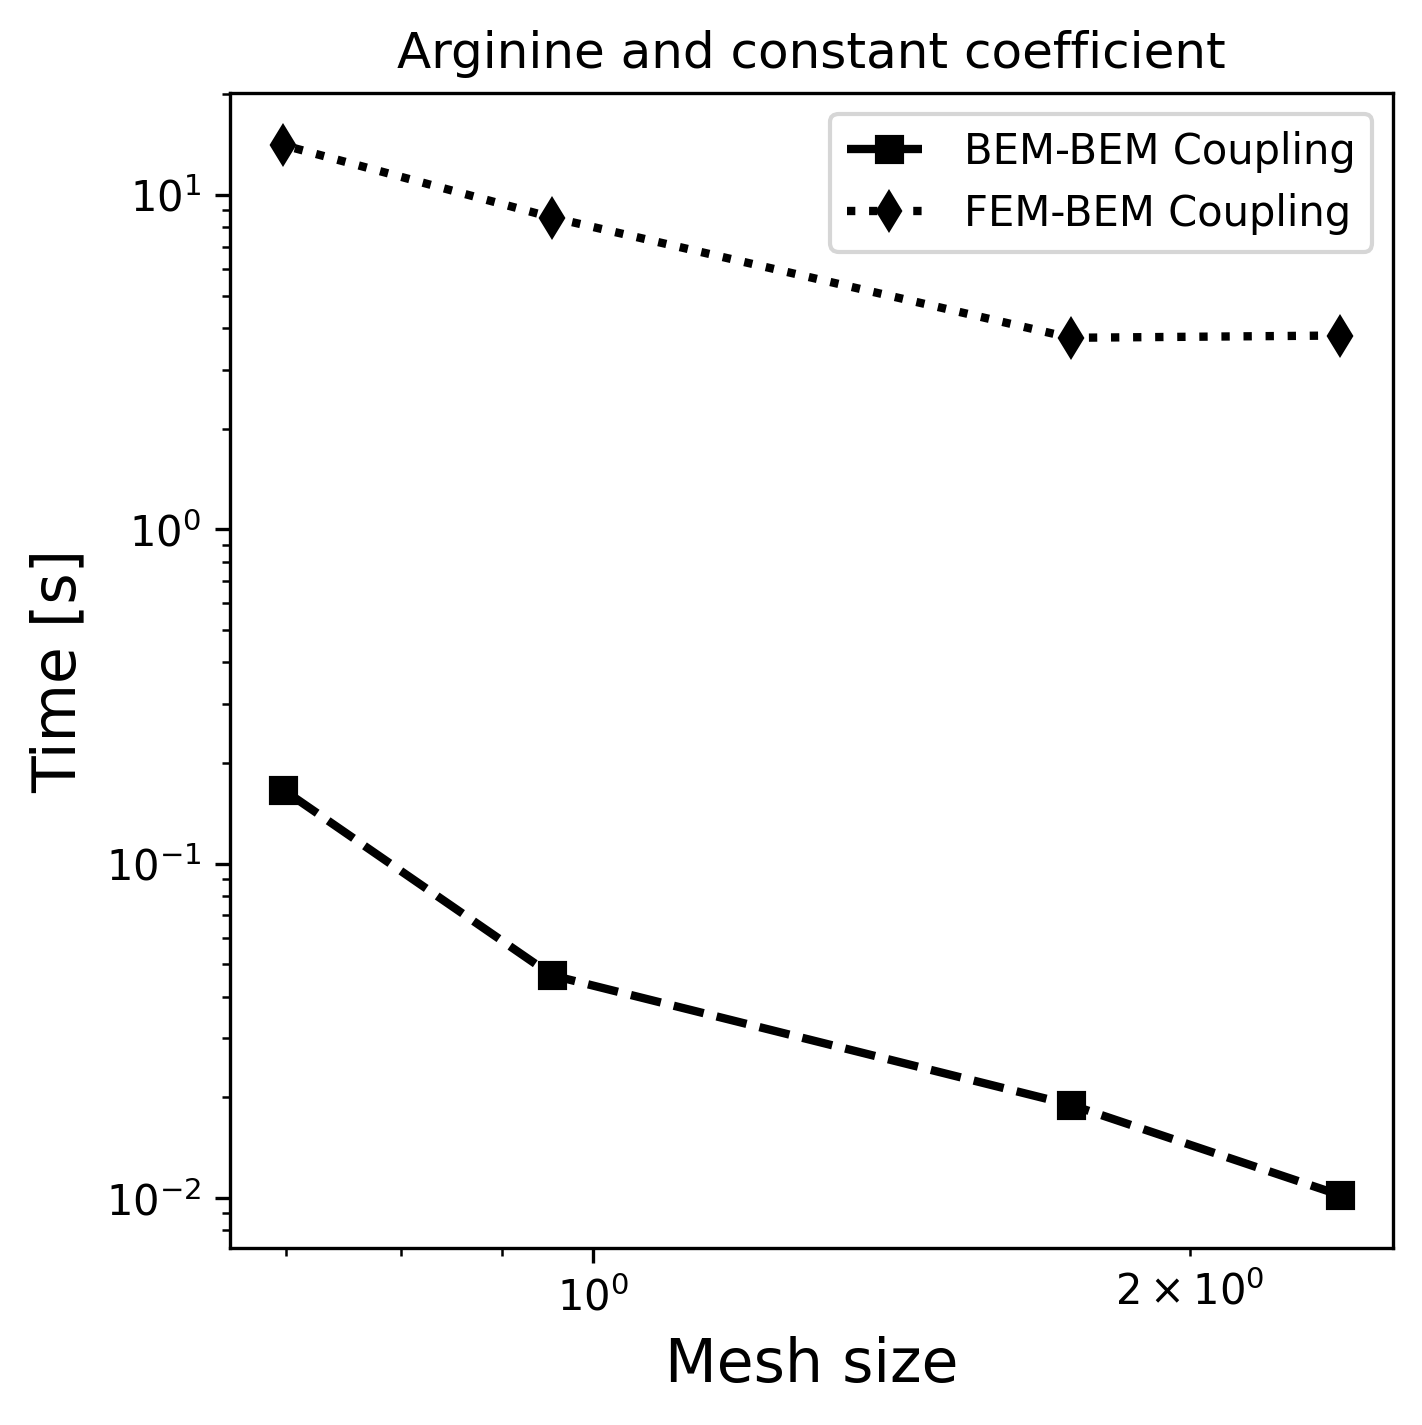
\includegraphics[width=0.45\linewidth]{DolfinX_Arginine_const_coeff_time_11.png}
%%  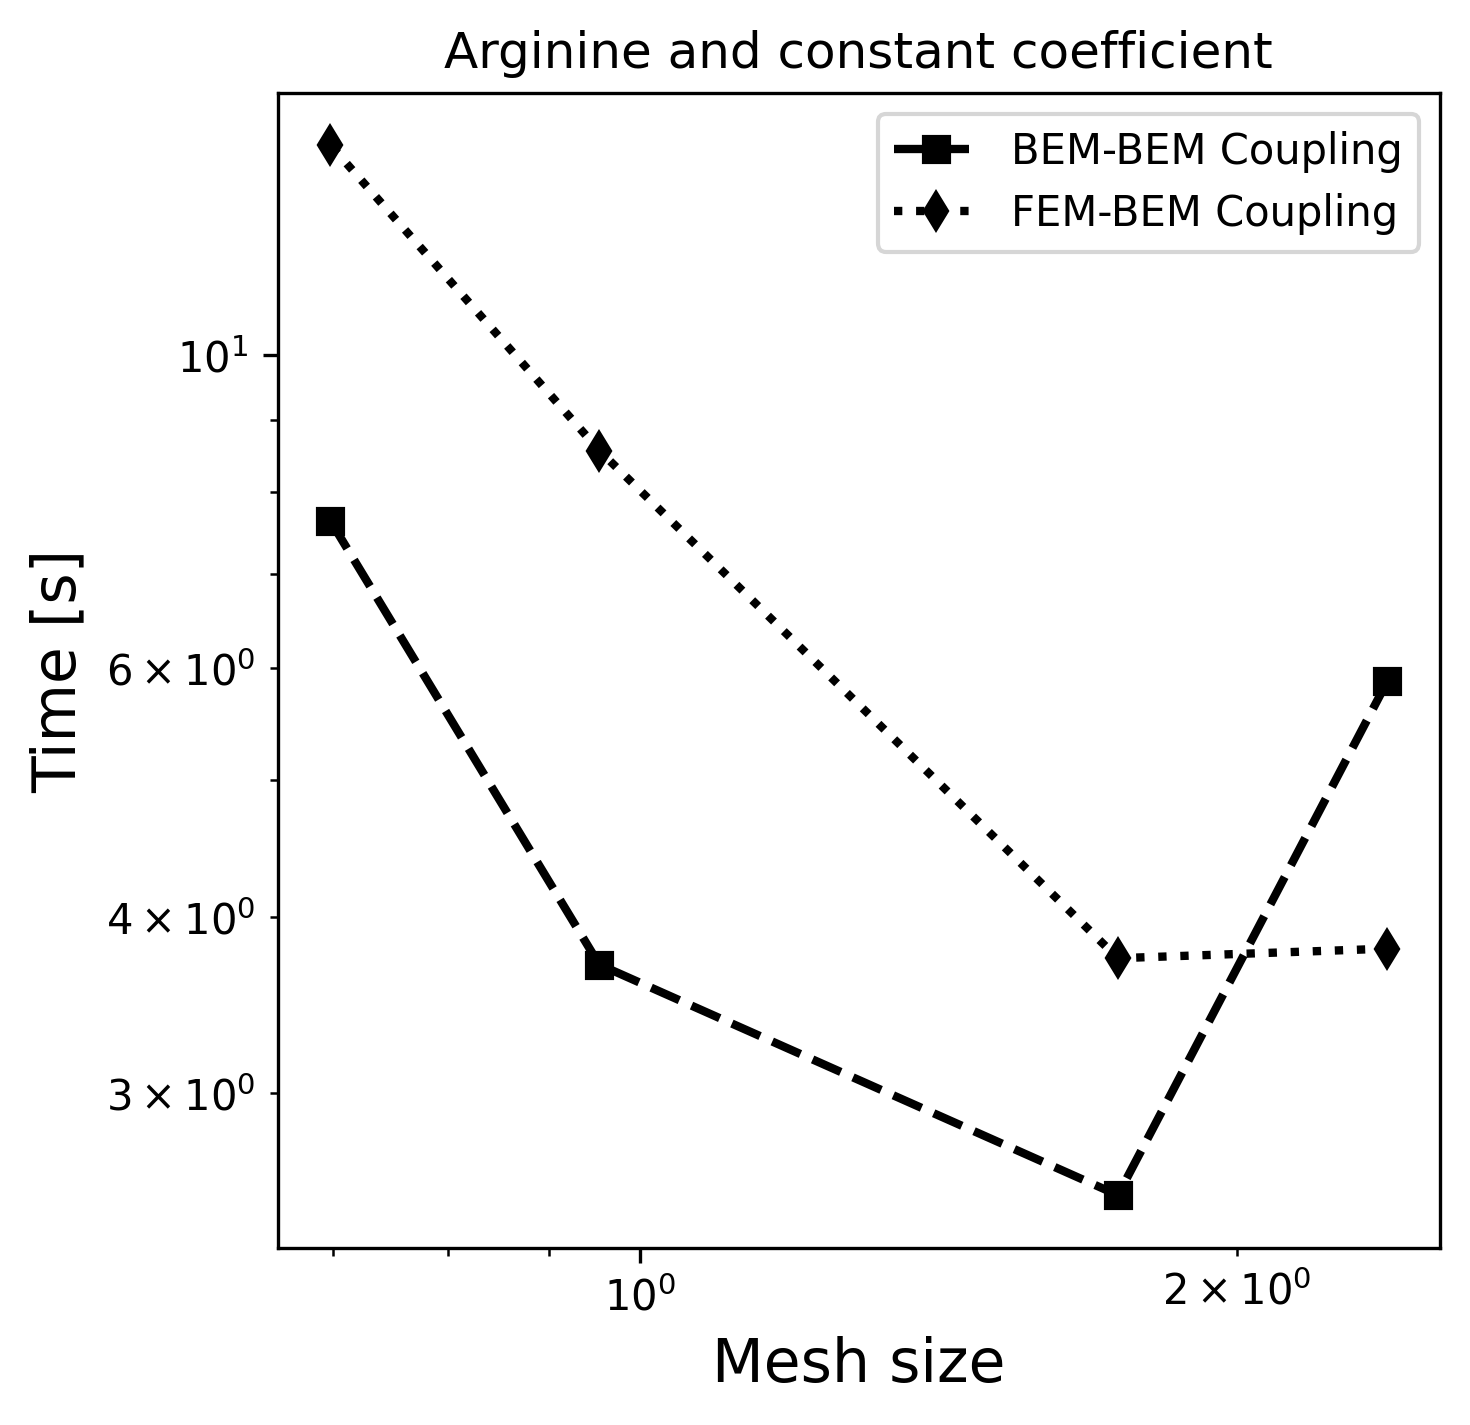
\includegraphics[width=0.45\linewidth]{DolfinX_Arginine_const_coeff_setup_time_11.png}
%  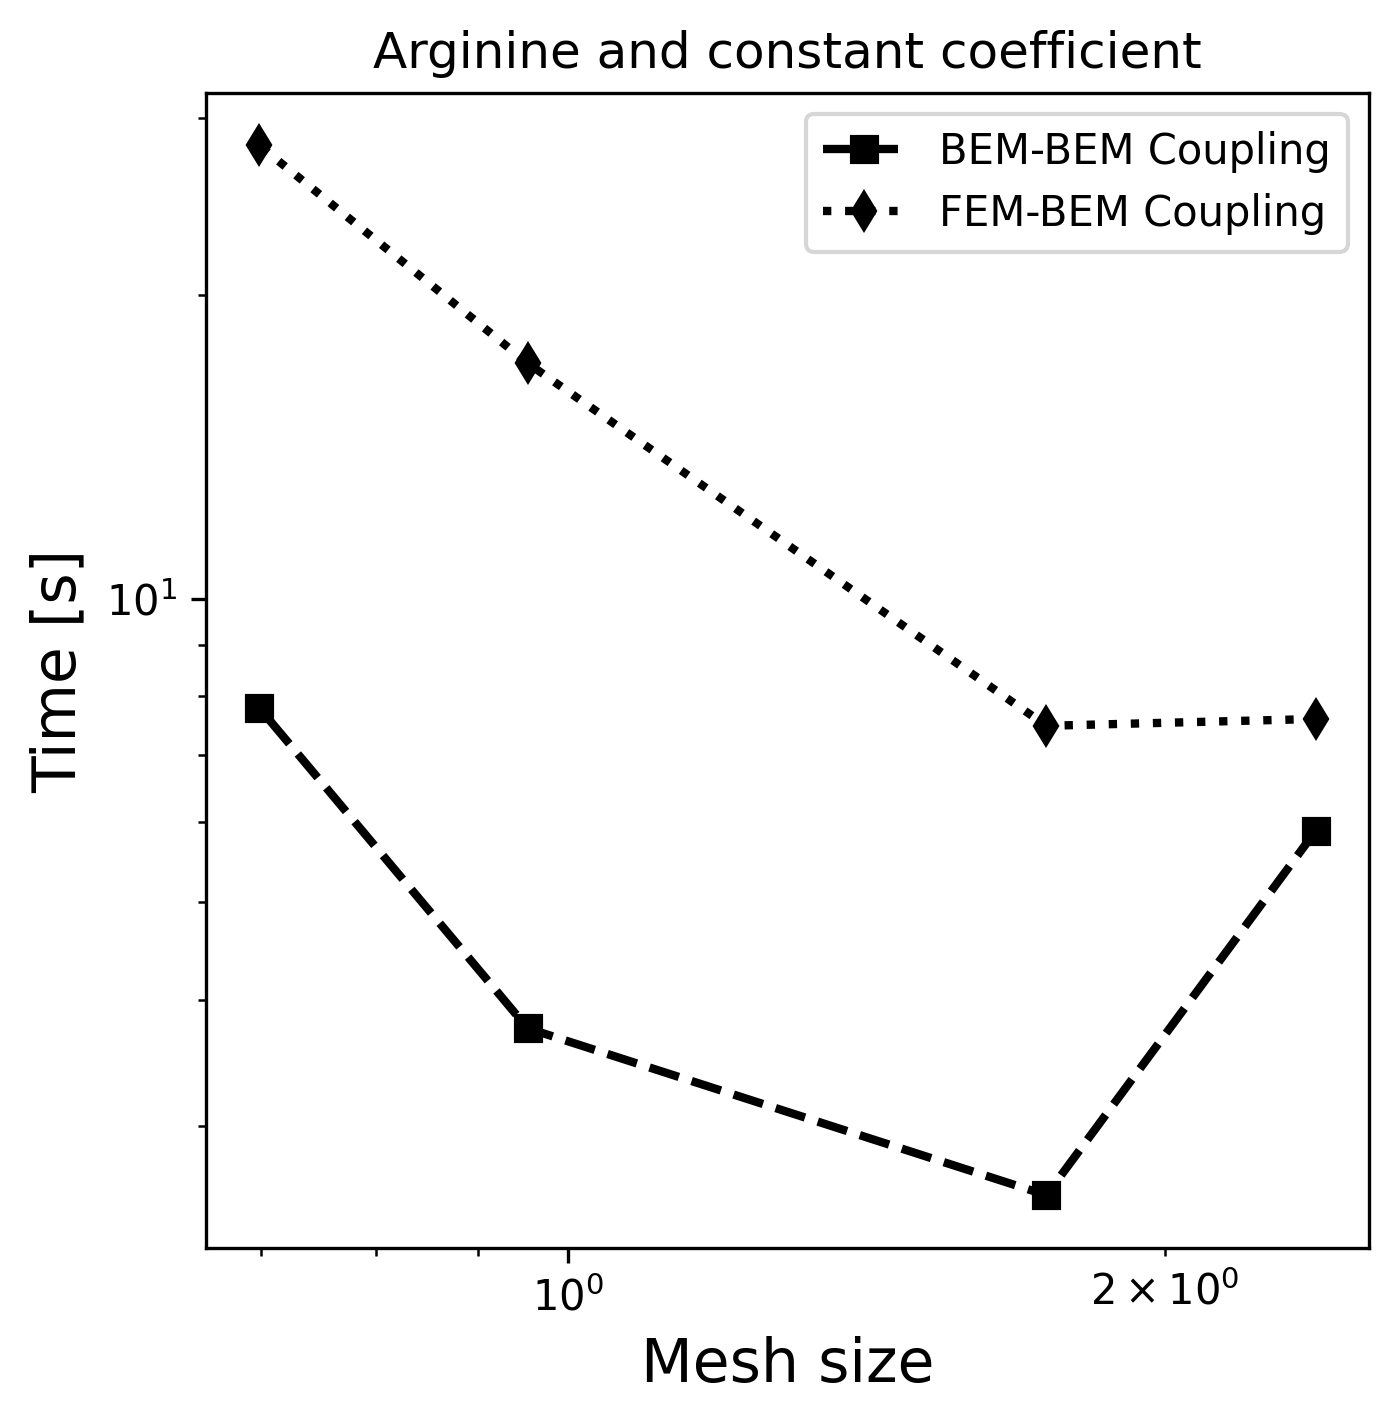
\includegraphics[width=0.45\linewidth]{DolfinX_Arginine_const_coeff_total_time_11.png}
%  \caption{Iteration count (left) and time-to-solution (right) for Arginine with a constant permittivity. %(left: Online time taken to solve systems, right: Offline time taken to set up systems). 
%%NOTE: x axis differ between top and bottom. Also, should we include preconditioned vs non preconditioned? We could easily precondition BEM-BEM too.  %(1) fix title, (2) can we put them in a single plot, (3) 
%%maybe we could also add a "error" wrt extrapolation, or a plot with energy for each mesh?
%}
%\label{fig:arg_constant_time_iter}
%\end{figure}


%\begin{figure}
%\centering
%%   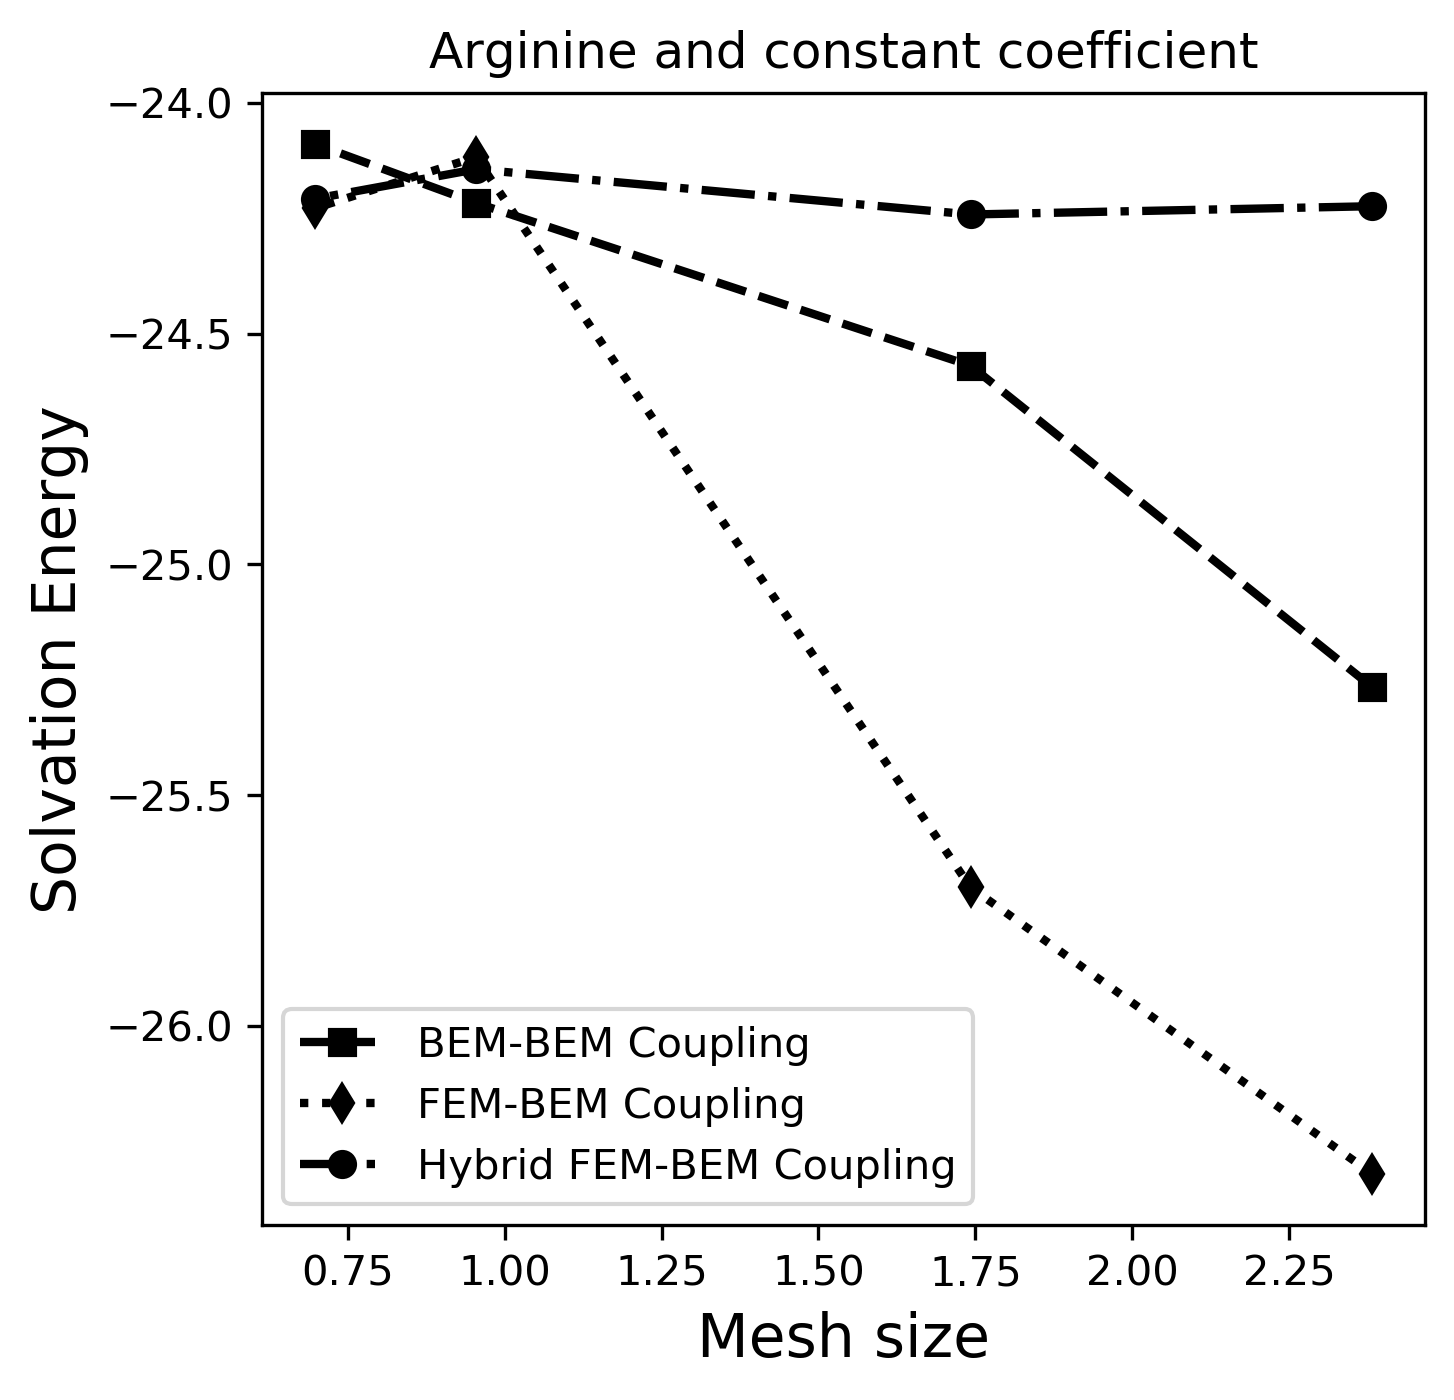
\includegraphics[width=0.45\linewidth]{Arginine_const_coeff_error.png}
%  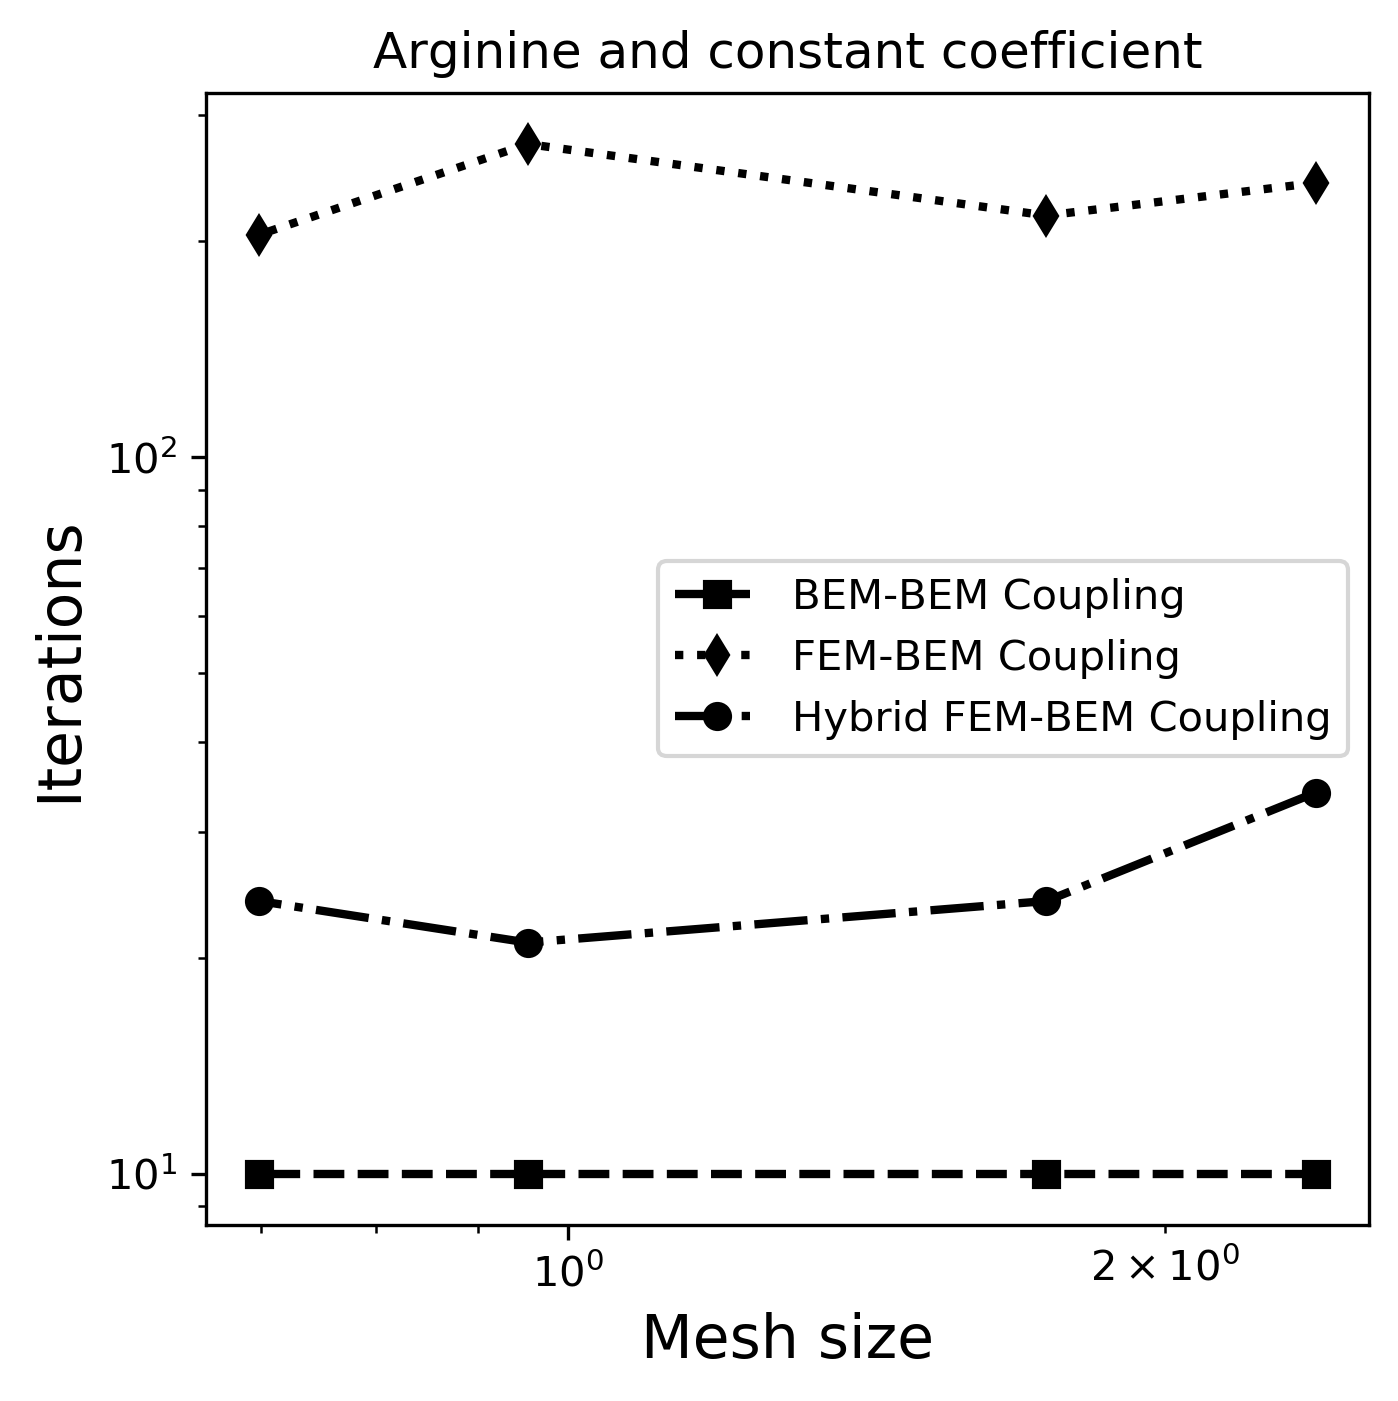
\includegraphics[width=0.45\linewidth]{Arginine_const_coeff_iter_11.png}
%%   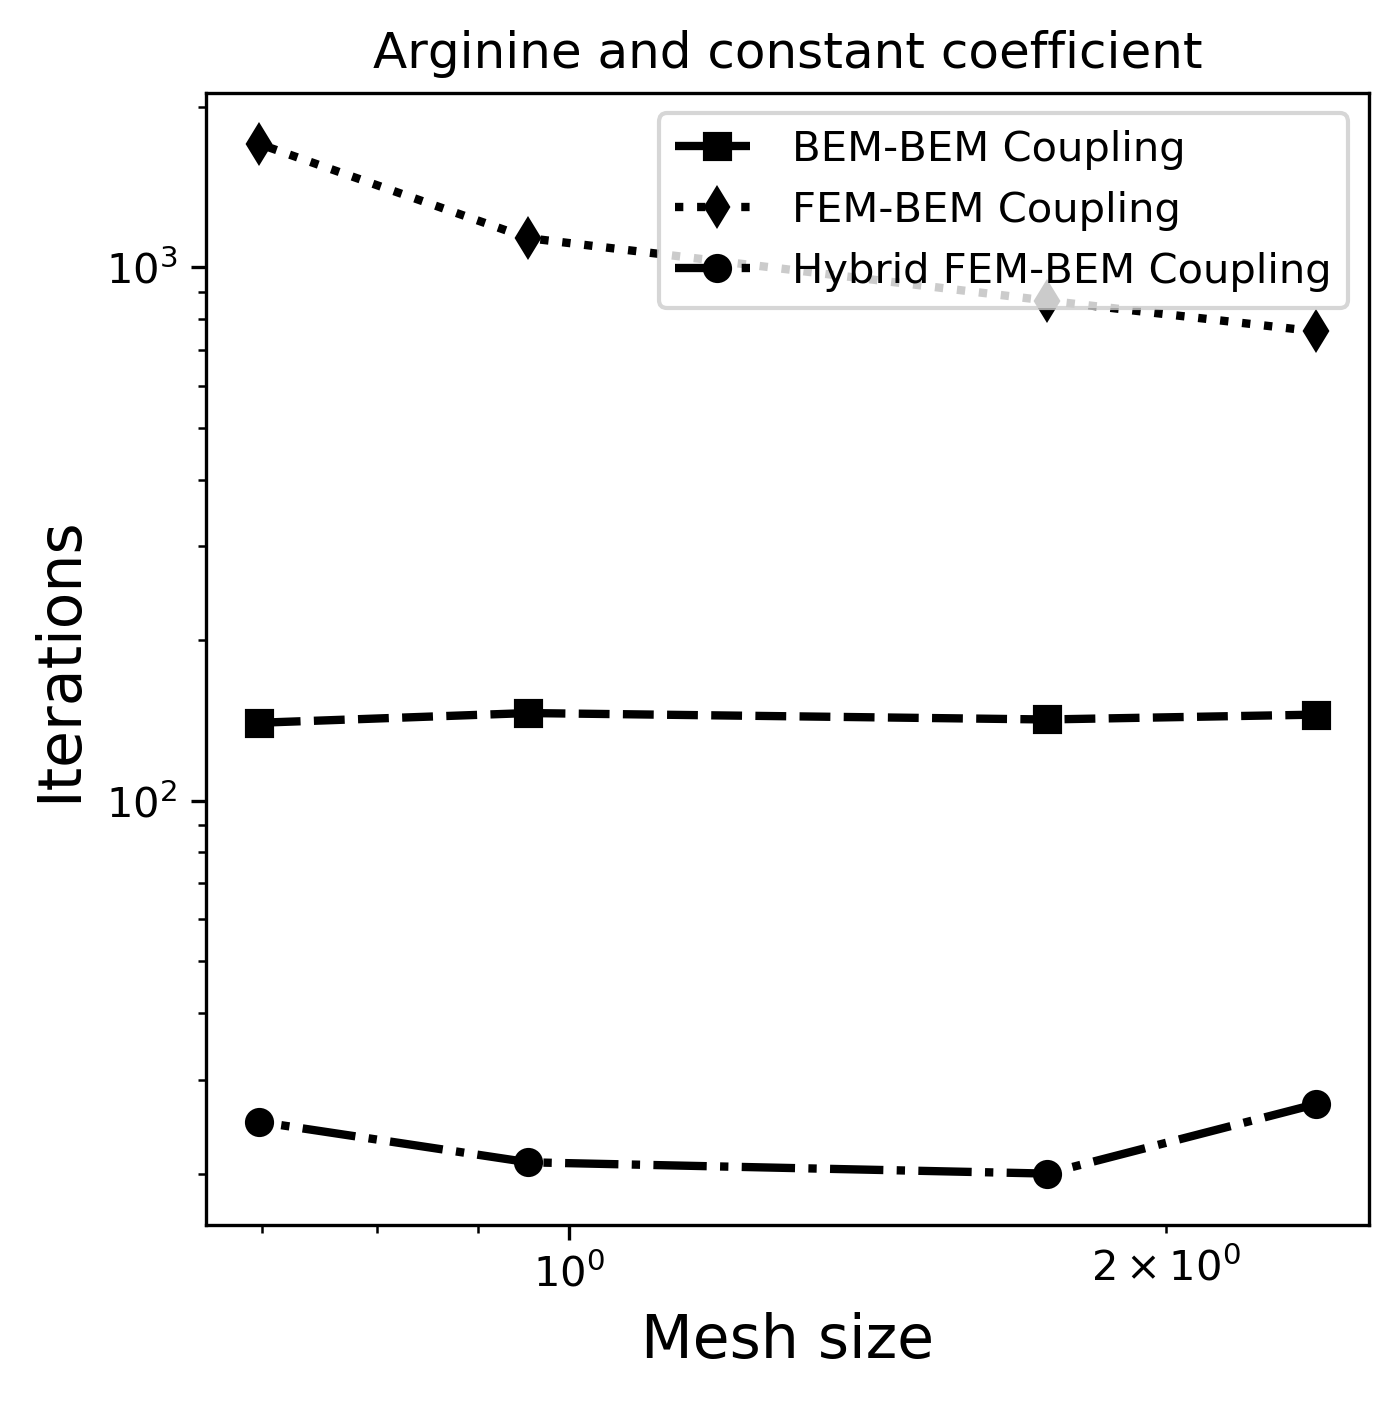
\includegraphics[width=0.45\linewidth]{No_prec_Arginine_const_coeff_iter.png}
%%   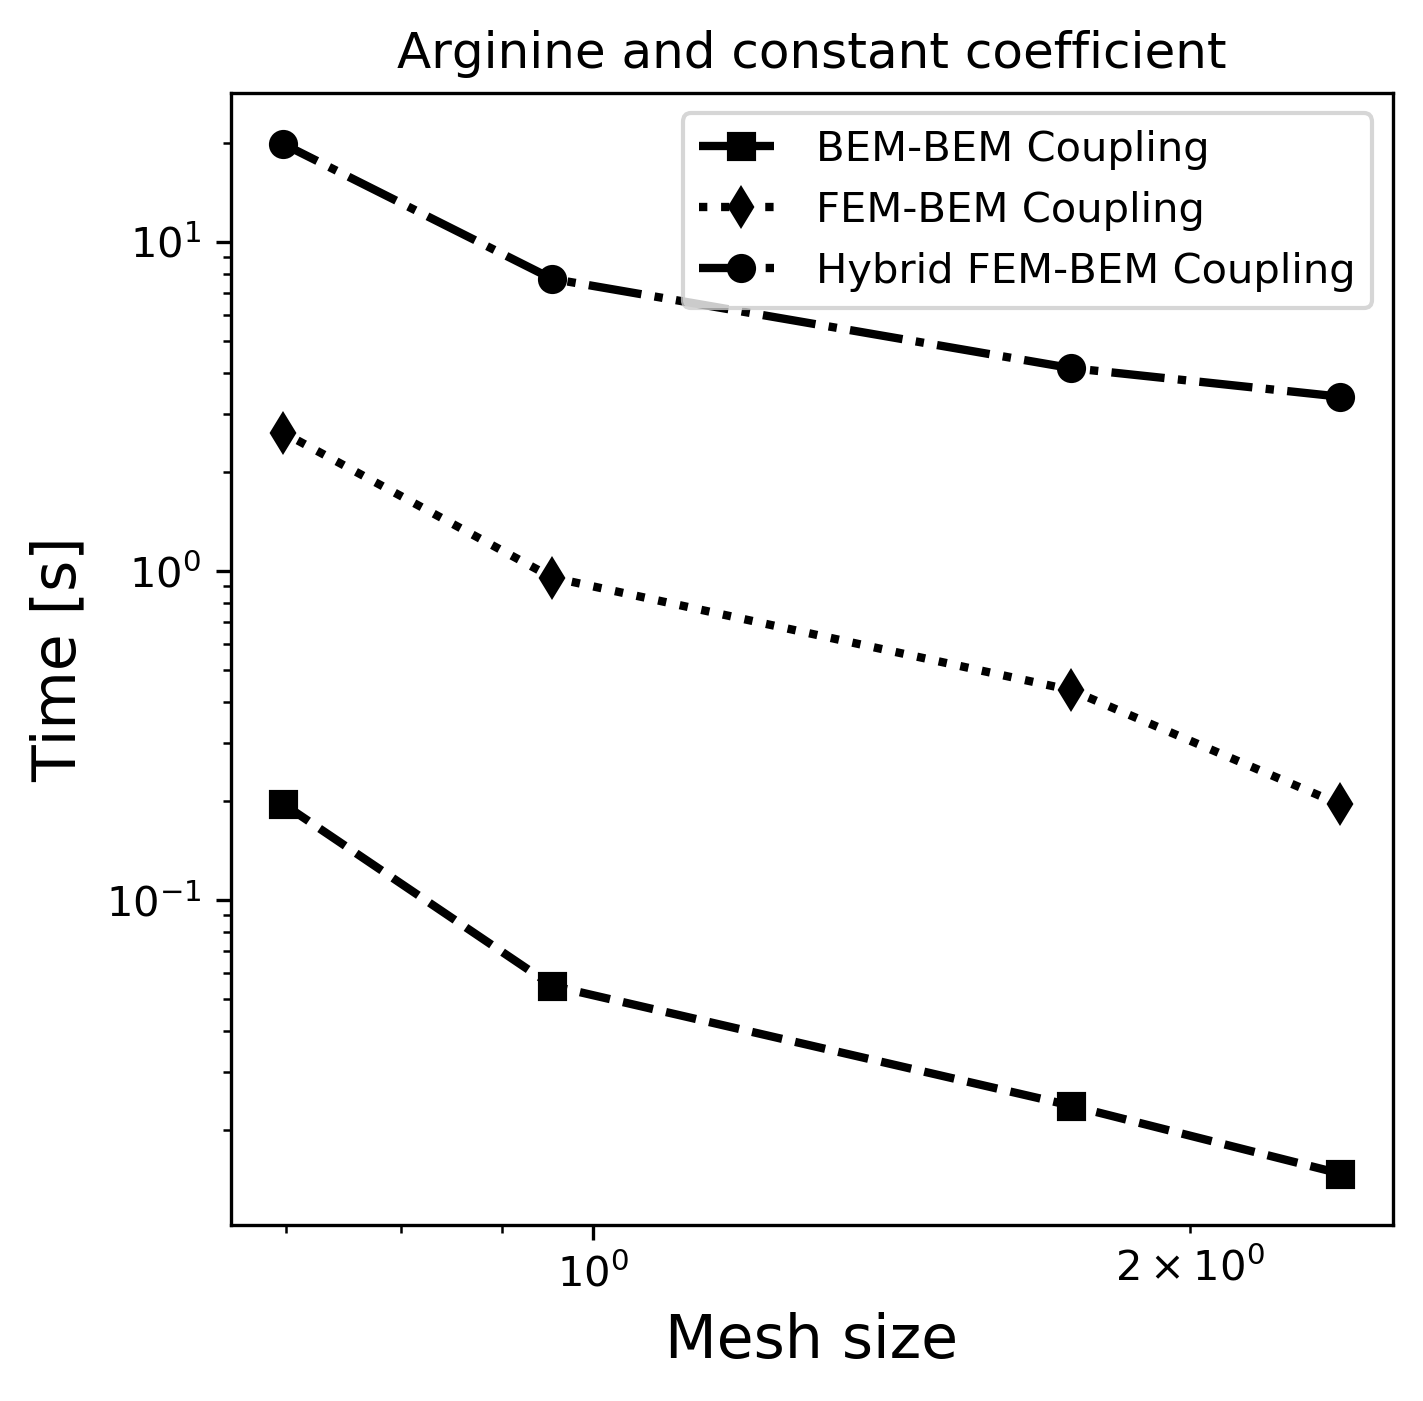
\includegraphics[width=0.45\linewidth]{Arginine_const_coeff_time.png}
%\caption{Iteration count for arginine with a constant permittivity. %(1) fix title, (2) can we put them in a single plot, (3) hybrid is internal or external iterations? maybe we should present the total count?
%}
%\label{fig:arg_contant_iter}
%\end{figure}



\section*{\sffamily \Large Results with variable permittivity}

\subsection*{\sffamily \large Motivation: modeling the solute with a Gaussian-based variable permittivity}

In contrast to a purely BEM approach, FEM-BEM coupling gives flexibility to consider space-varying field parameters. 
A popular description of the molecule is to consider a permittivity that varies like a Gaussian around each atom,\cite{grant2001smooth} which has shown enhanced accuracy in some applications, like pKa calculations.\cite{li2013dielectric}
In this setting, we define a density function $\rho$ depending on position $r$ as
%
\begin{equation}
\rho(r) := \prod_i \left(1 - \exp{\left(\frac{\|r-\mathbf{x}_i\|}{\sigma^2 R_i^2}\right)}\right)
\end{equation}
%
where the product runs over all the atoms of the solute, $R_i$ is the van der Waals radius of atom i, and we used $\sigma$=1. Then, we can compute the permittivity as
%
\begin{equation}\label{eq:varying_eps}
\epsilon := \left(1-\rho \right) \epsilon_1 + \rho\epsilon_2
\end{equation}

As $\epsilon$ is variable, Equation \eqref{eq:phic} does not have an analytical solution, and the electrostatic potential in the vacuum state has to be computed numerically.
For vacuum calculations, we considered the same distribution of $\epsilon$ inside the molecule as in the solvated case, but the solvent permittivity was set to $\epsilon_2$=2. 
Other implementations of Gaussian permittivities also modify the solute permittivity in vacuum calculations, according to a set cutoff.\cite{li2013dielectric} We did not consider a cutoff in our calculations.


We used Equation \eqref{eq:varying_eps} to generate dielectric maps, which we ran on APBS~\cite{BakerETal2001} for comparison. 
We chose APBS because it provides an easy interface to control dielectric maps, in order to ensure their agreement with the maps imposed in our FEM-BEM coupled approach.

\subsection*{\sffamily \large Convergence and performance for arginine}

Table \ref{table:arg_variable} shows a comparison of solvation energy computed with APBS and our FEM-BEM coupling approach. We can see that they are both converging to equivalent values, where the finest meshes agree up to 0.5\% (0.5 kcal/mol).

Figure \ref{fig:arg2_variable} contains the performance results of this test case, where we distinguish the iteration count from the calculation in dissolved and vacuum states. 

\begin{table}
\centering
\begin{tabular}{c|c|c|c}
&Mesh size  & Grid points & $\Delta G_{solv}$\\
&\AA       & &  kcal/mol \\
\hline
\multirow{4}{*}{APBS}& 0.52$\times$0.52$\times$0.52 & 97$\times$97$\times$97 & -107.6186 \\ 
& 0.39$\times$0.39$\times$0.39 & 129$\times$129$\times$129 & -107.8752\\ 
&0.26$\times$0.26$\times$0.26 & 193$\times$193$\times$193& -108.3378\\ 
&0.195$\times$0.195$\times$0.195 & 257$\times$257$\times$257& -108.5837\\ 
&0.098$\times$0.098$\times$0.098 & 513$\times$513$\times$513& -108.8844\\ 
\hline
&Mesh dens. & DOFs & $\Delta G_{solv}$\\
&vert/\AA$^2$   &  &  kcal/mol \\
\hline
%\multirow{5}{*}{Standard FEM-BEM}& 2 & -36.239\\
    & 4.1 & 3 491 & -109.933 \\
FEM-BEM    & 6.7  & 5 787 & -110.238 \\
coupling    & 8.57  & 8 844 & -109.658 \\
    & 17 & 19 911 & -109.368 \\
    & 24.5 & 32 302 & -109.286 \\
\hline
%\multirow{5}{*}{Standard FEM-BEM}& 2 & -29.554\\
%    & 2 & -34.670\\
%Hybrid    & 4  & -33.603 \\
%FEM-BEM    & 8  & -32.822 \\
%    & 16 & -32.072 \\
%\hline
\end{tabular}
\caption{Solvation energy of arginine with a Gaussian-like permittivity, computed using the FEM-BEM approach and APBS. The mesh density for FEM-BEM corresponds to the vertex density of the surface mesh used to generate the volumetric mesh.}
\label{table:arg2_variable}
\end{table}

%\begin{figure}
%\centering
%% 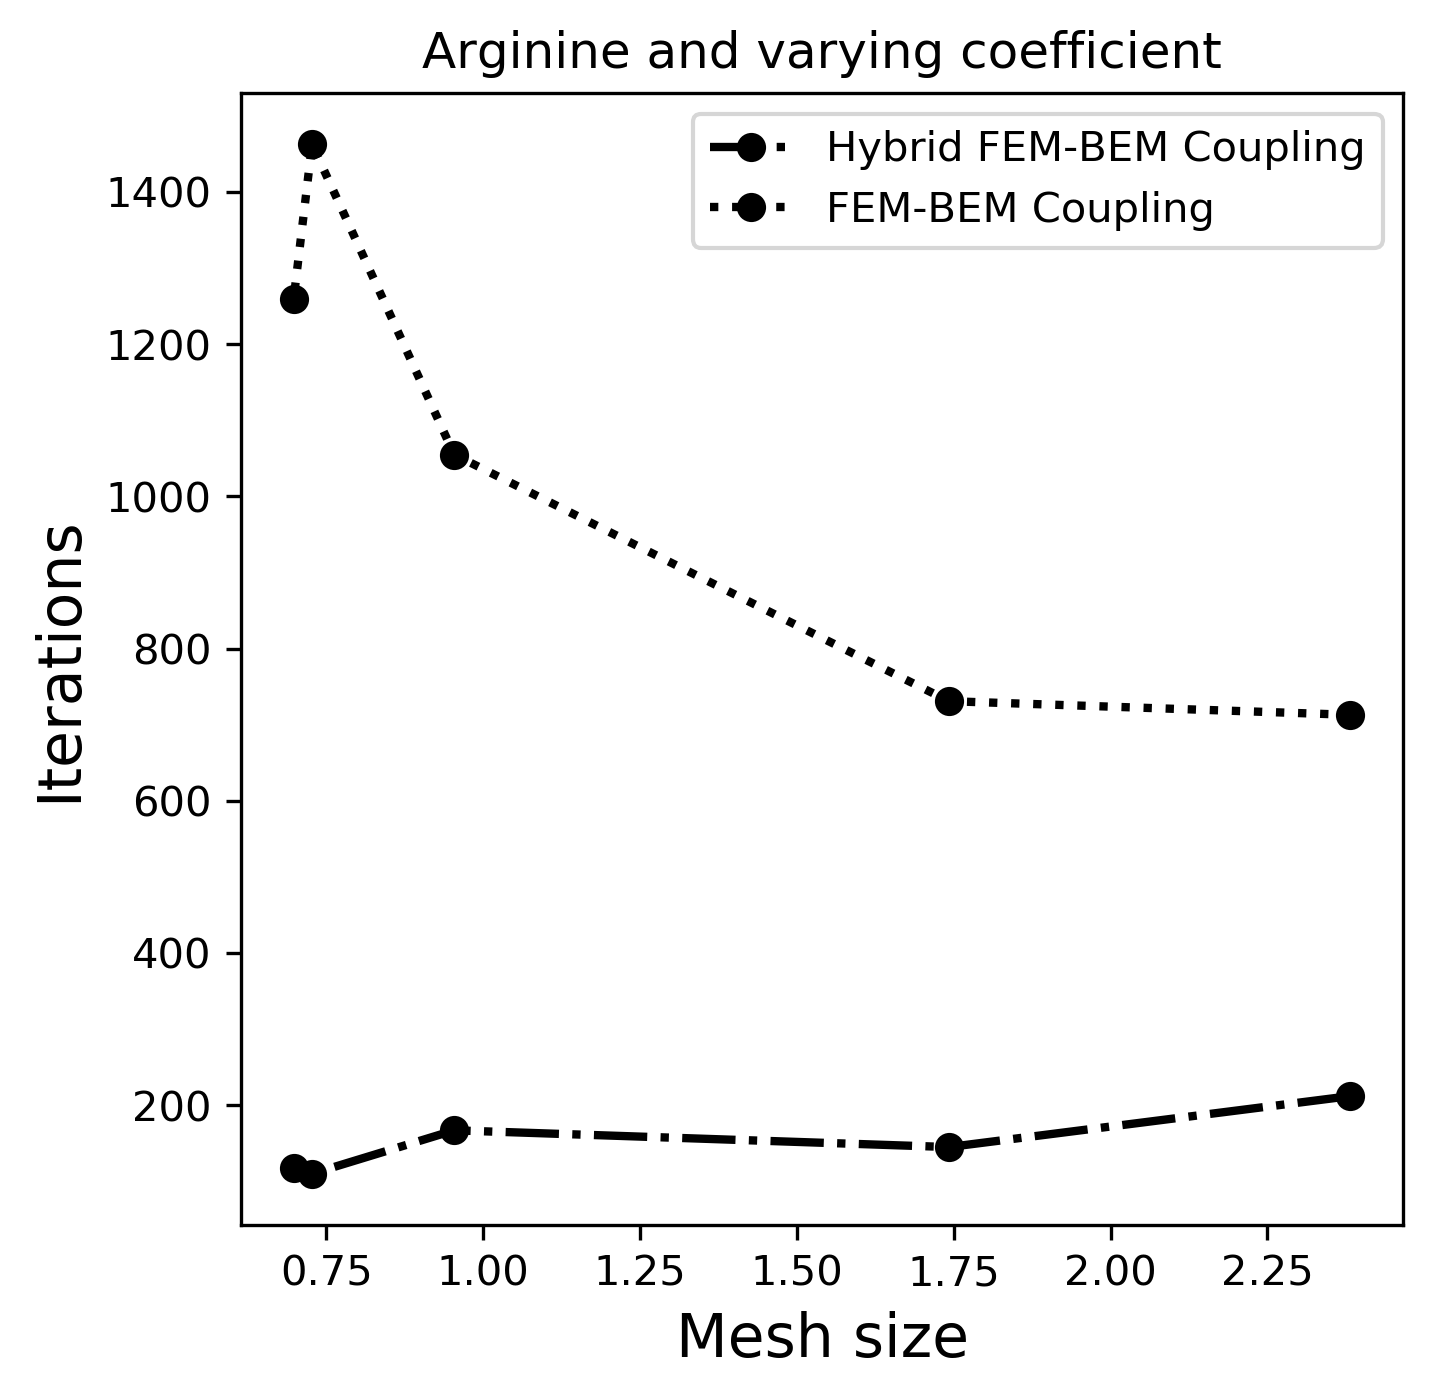
\includegraphics[width=0.45\linewidth]{Arginine_varying_coeff_iter.png}
%% 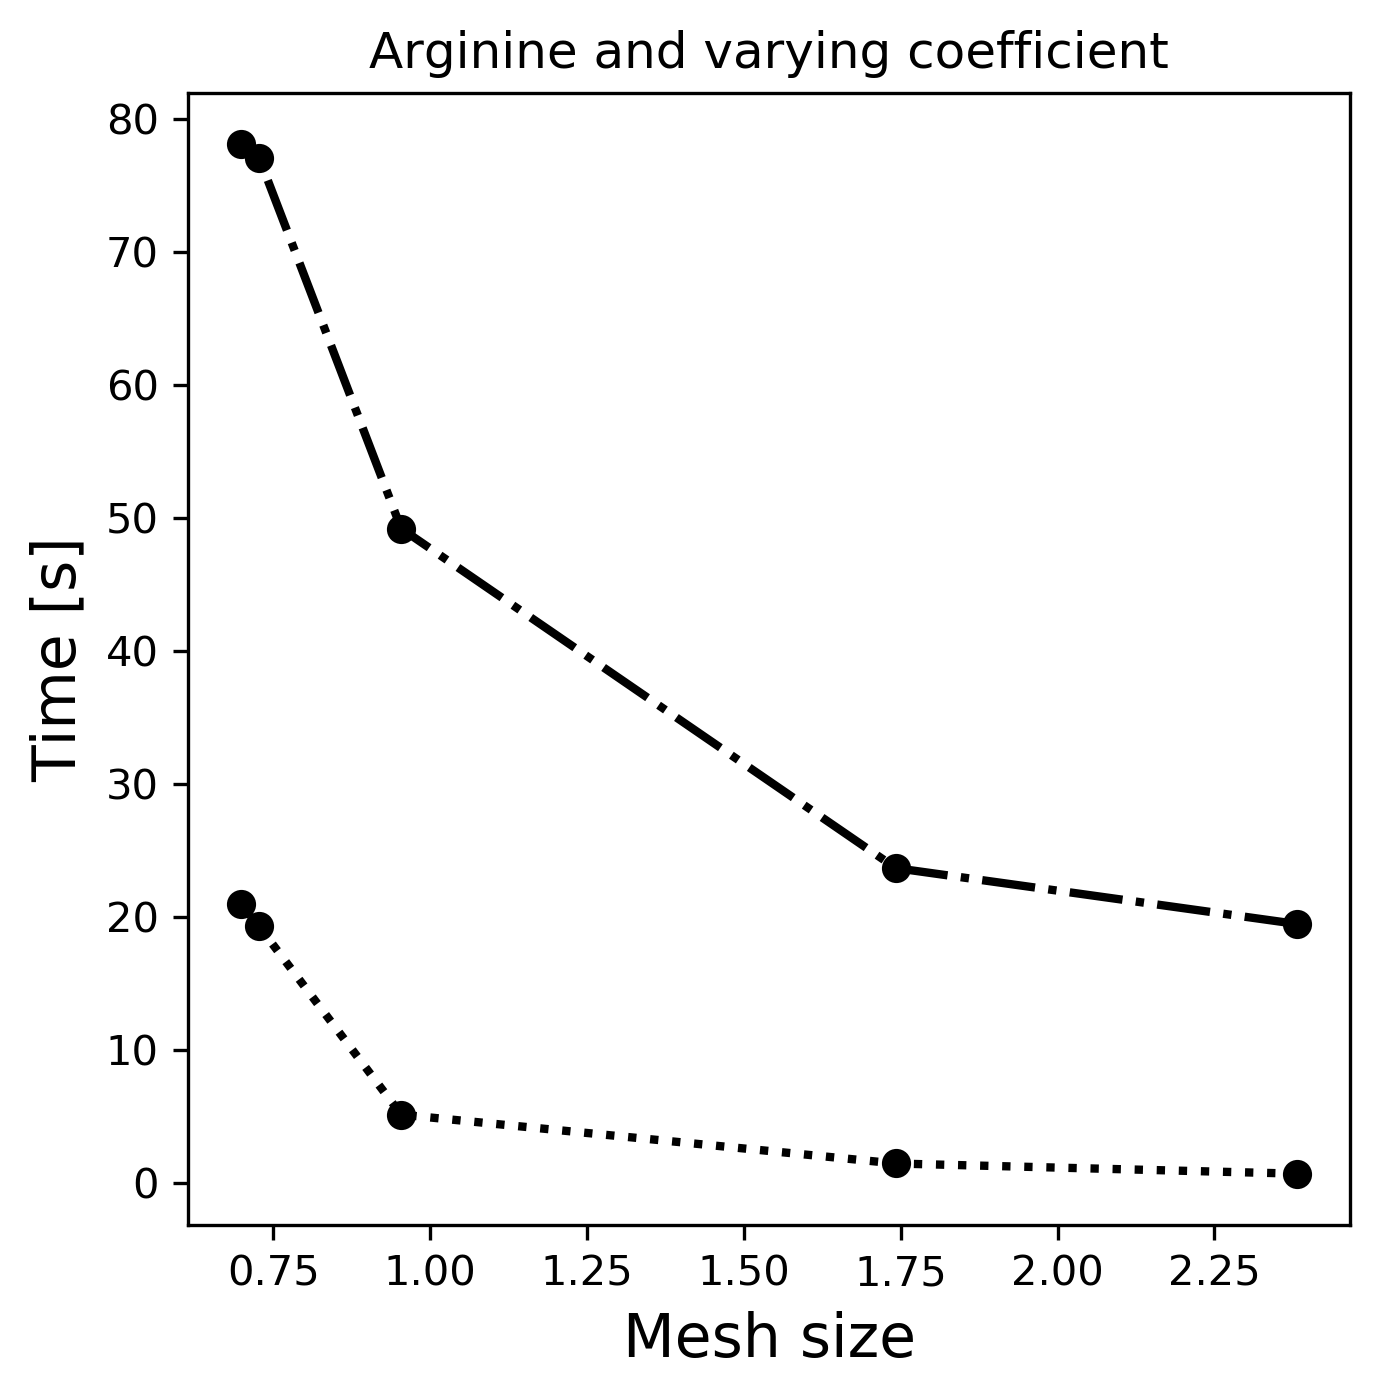
\includegraphics[width=0.45\linewidth]{Arginine_varying_coeff_time.png}
%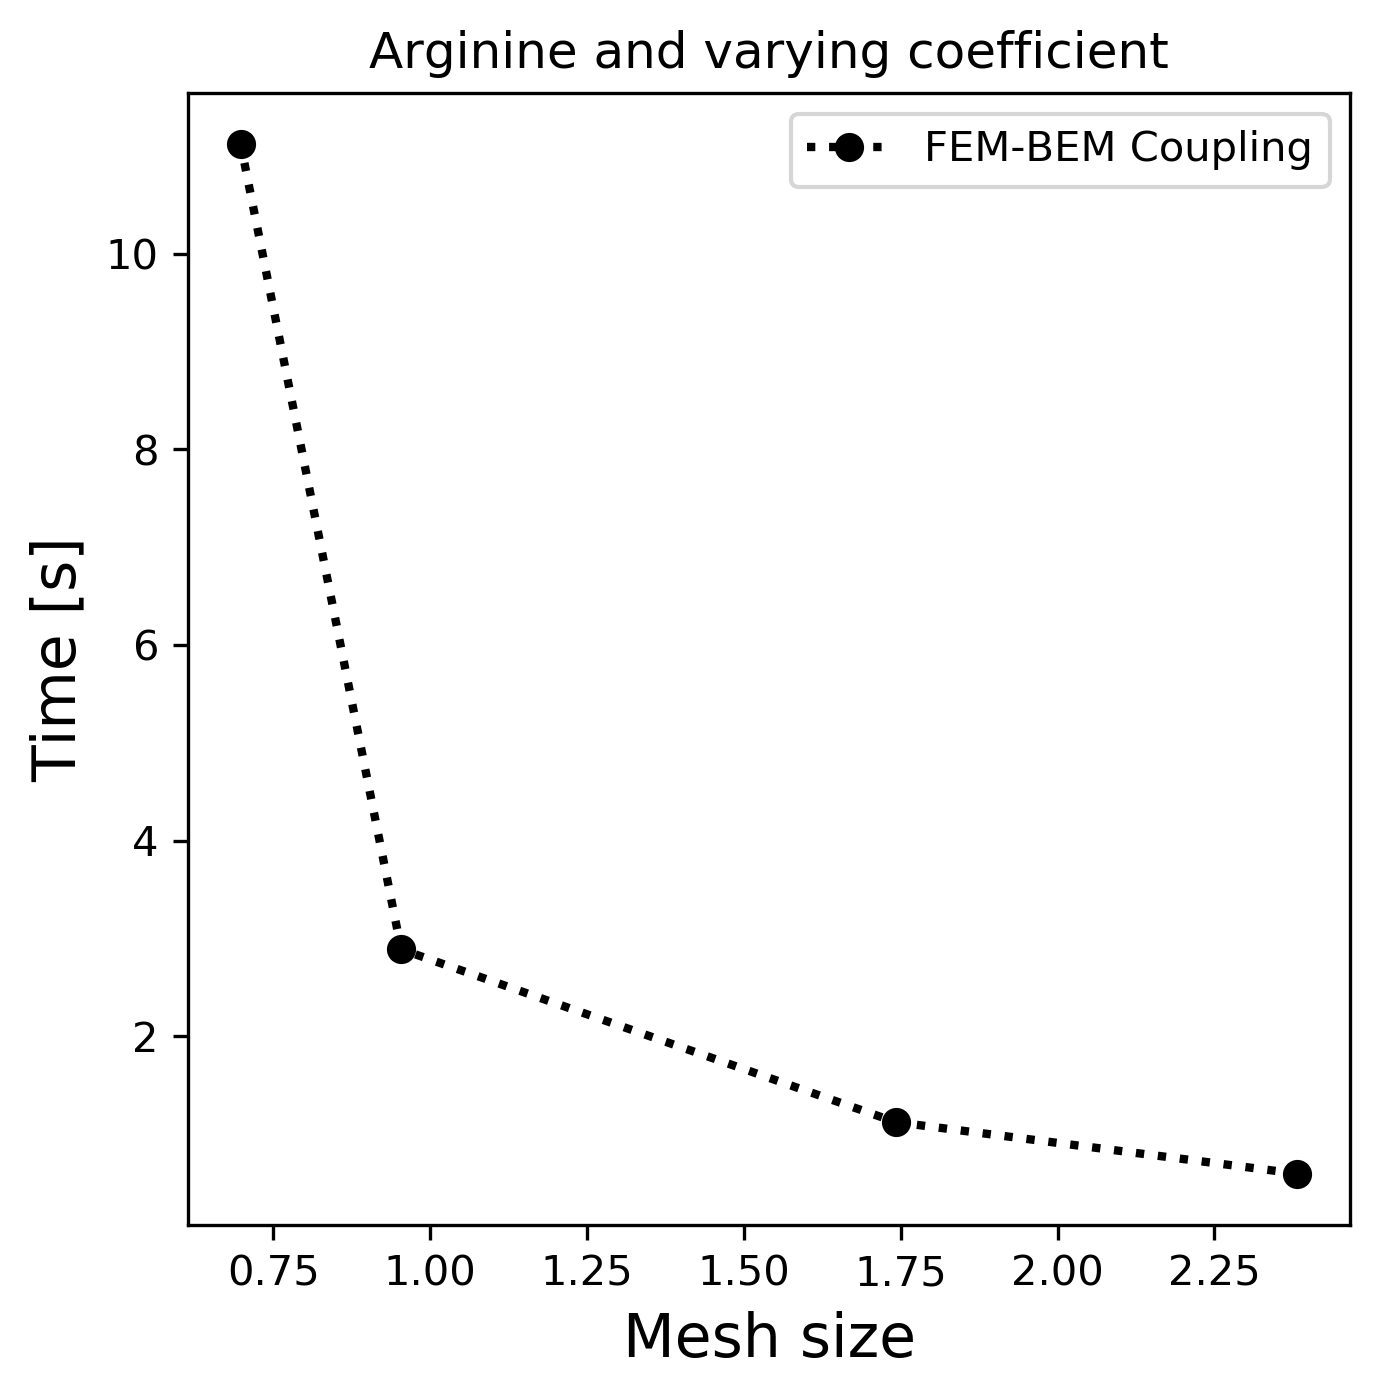
\includegraphics[width=0.45\linewidth]{Arginine_varying_coeff_time_11.png}
%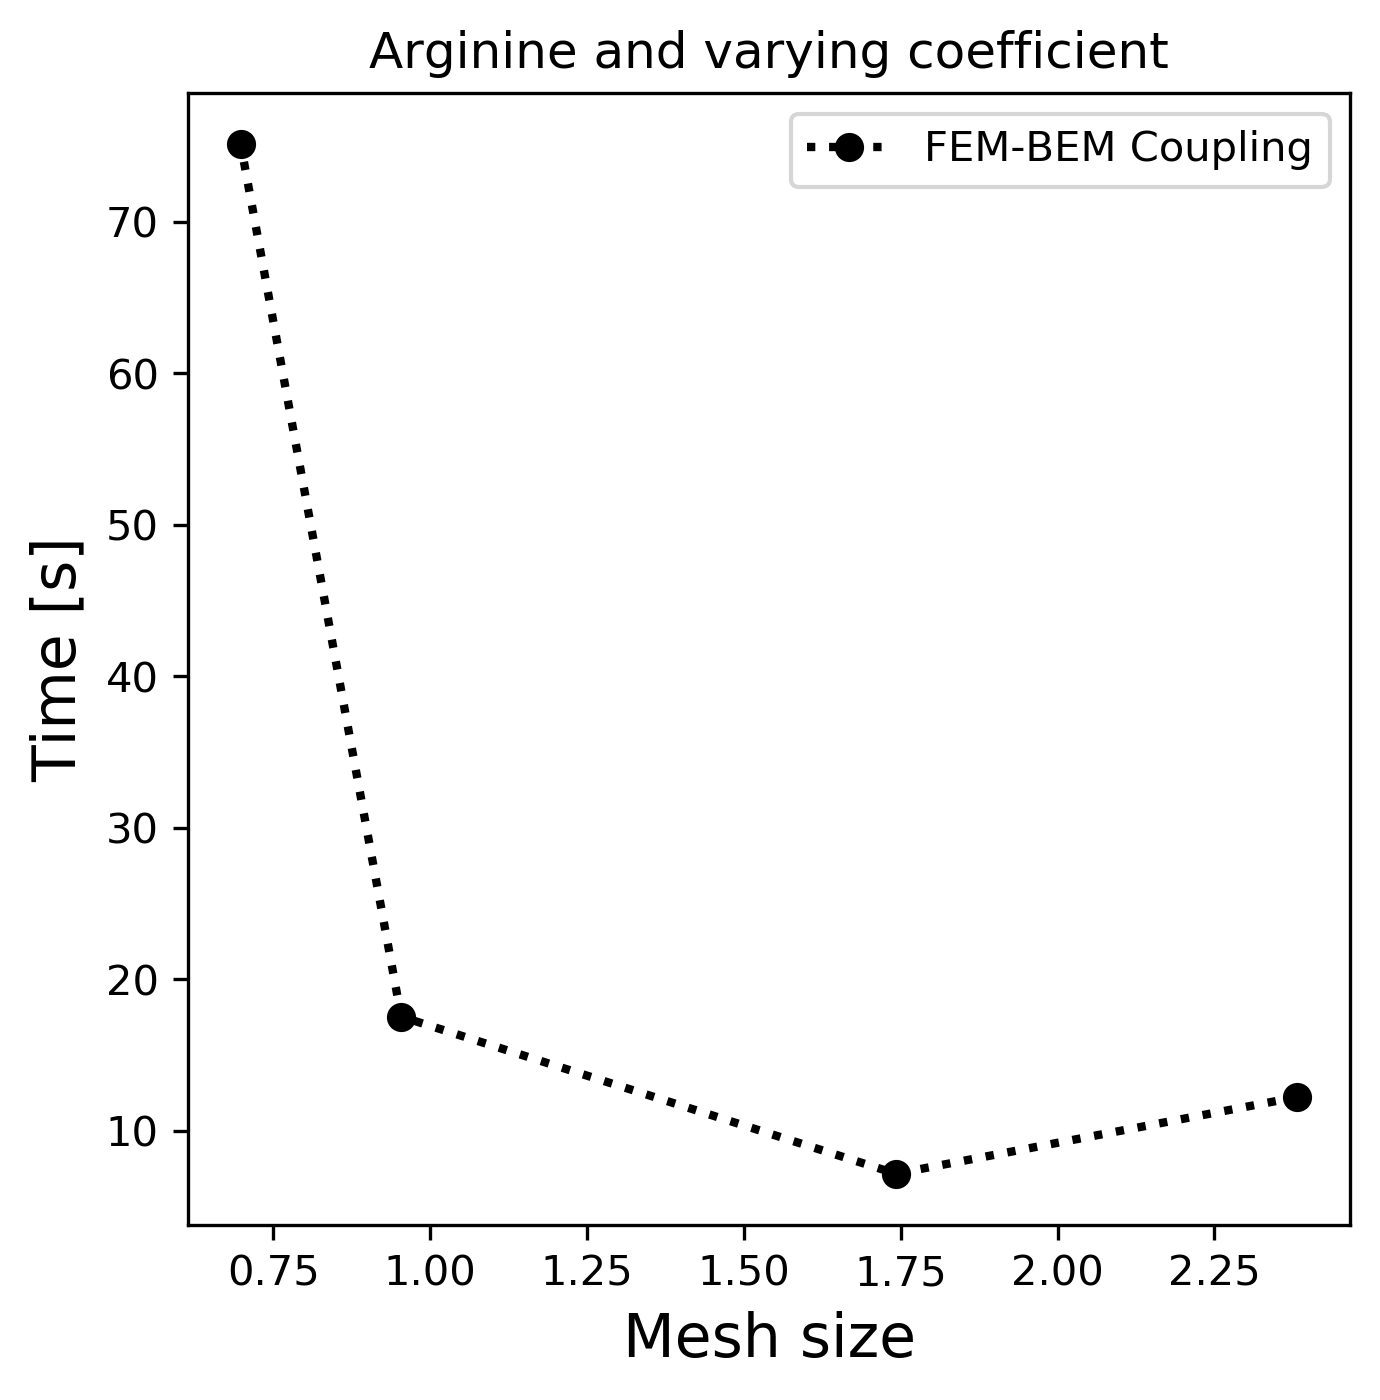
\includegraphics[width=0.45\linewidth]{Arginine_varying_coeff_setup_time_11.png}
%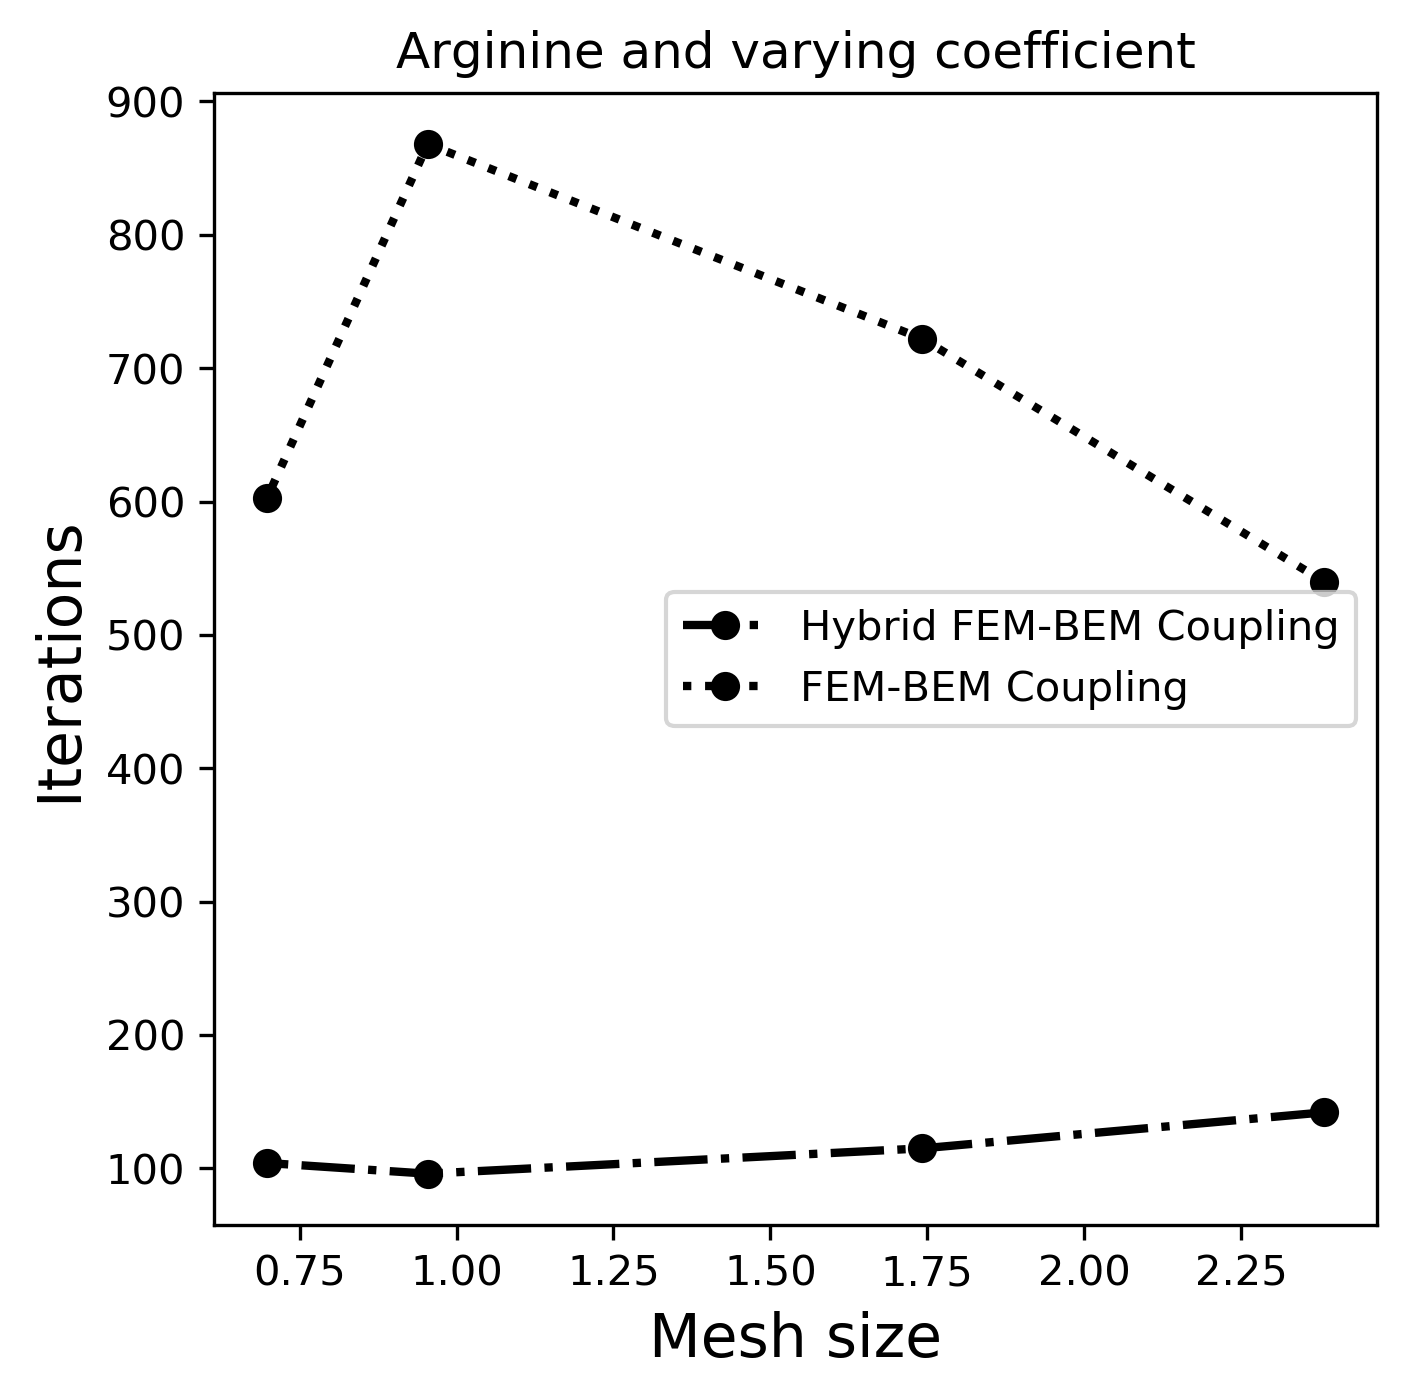
\includegraphics[width=0.45\linewidth]{Arginine_varying_coeff_iter_11.png}
%\caption{Iteration count and time-to-solution to compute the solvation energy of arginine with a variable permittivity (left: Online time taken to solve systems, right: Offline time taken to set up systems), using FEM-BEM coupling. %Can we make this only two plots?
%}
%\label{fig:arg_variable}
%\end{figure}

\begin{figure}
\centering
% 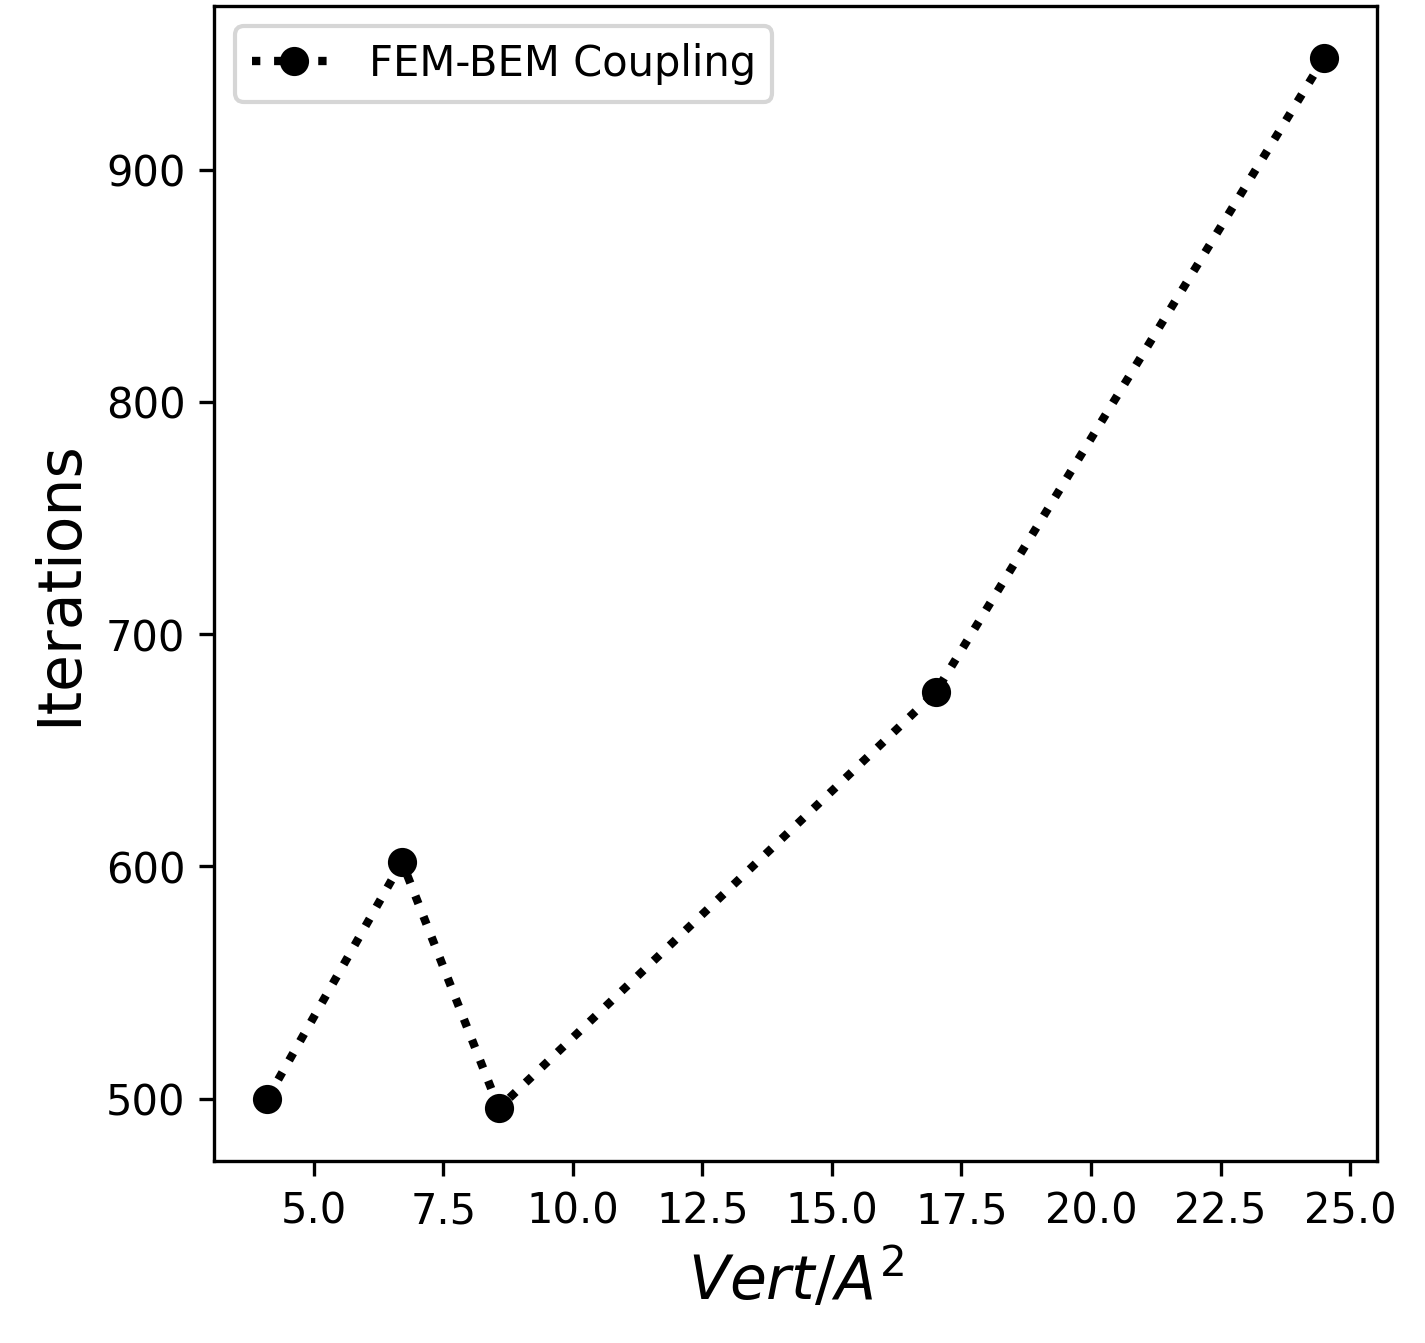
\includegraphics[width=0.45\linewidth]{DolfinX_Arginine2_varying_coeff_iter.png}
% 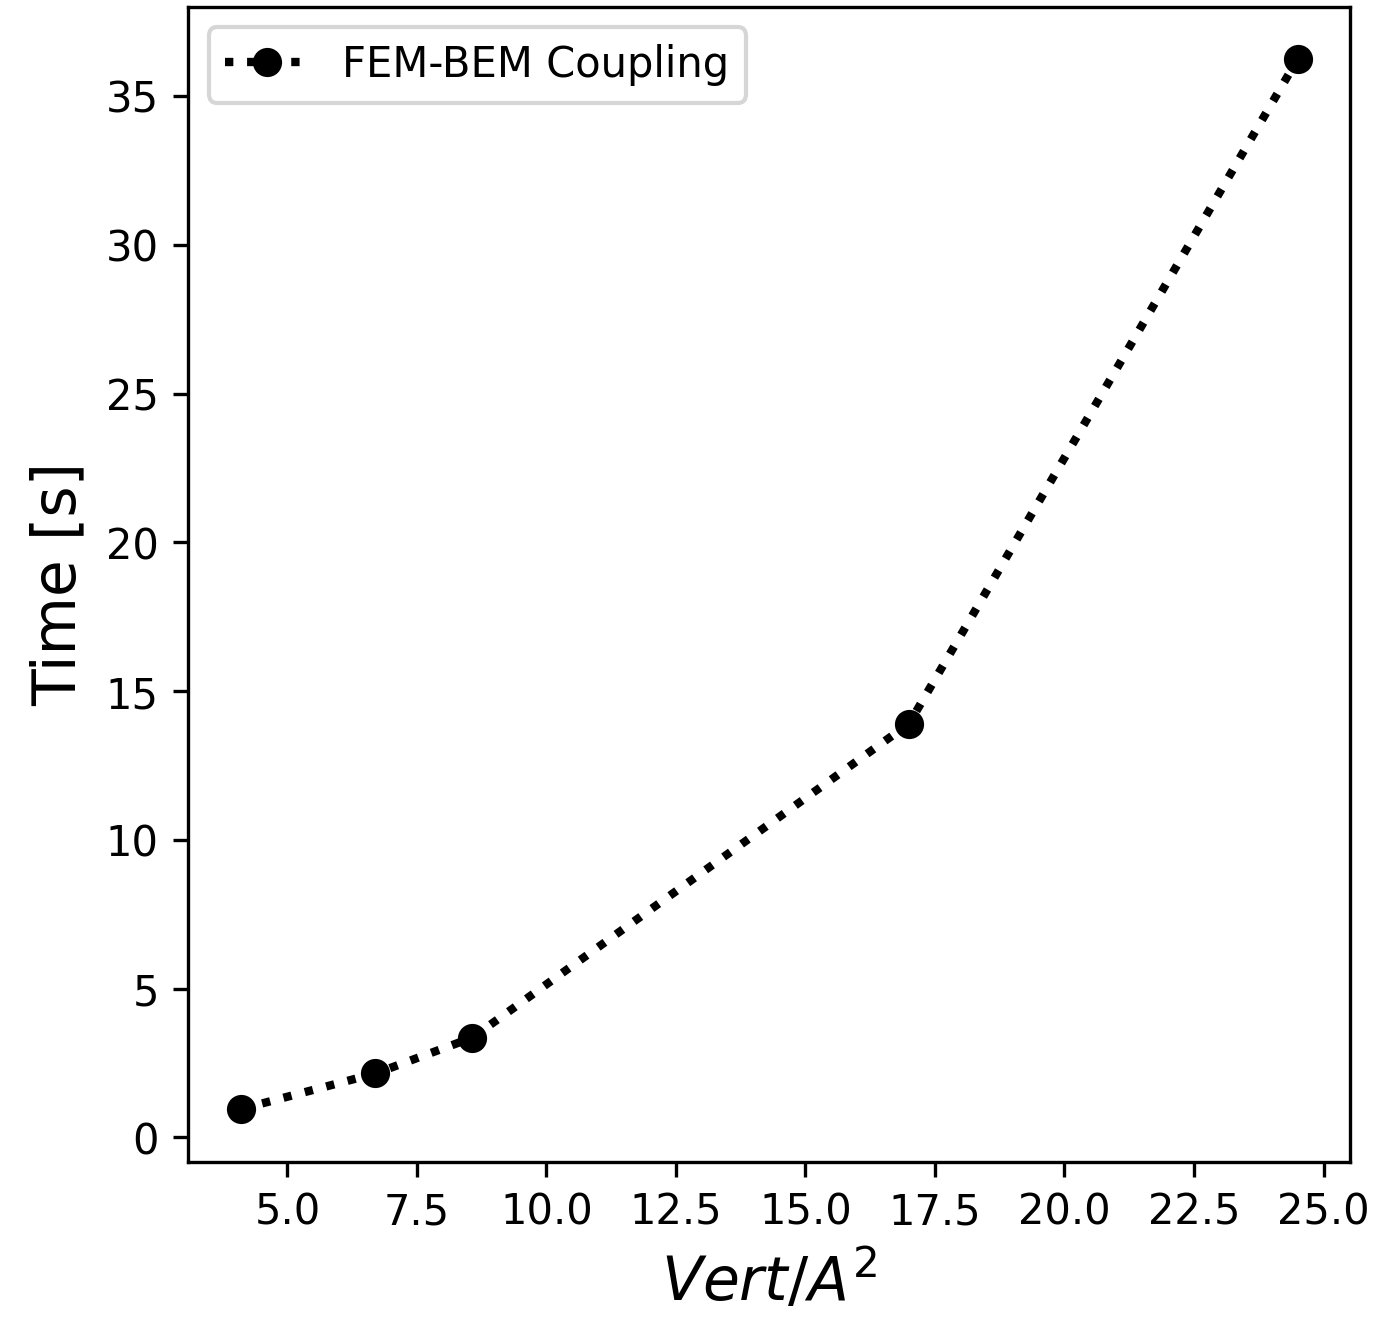
\includegraphics[width=0.45\linewidth]{DolfinX_Arginine2_varying_coeff_time.png}
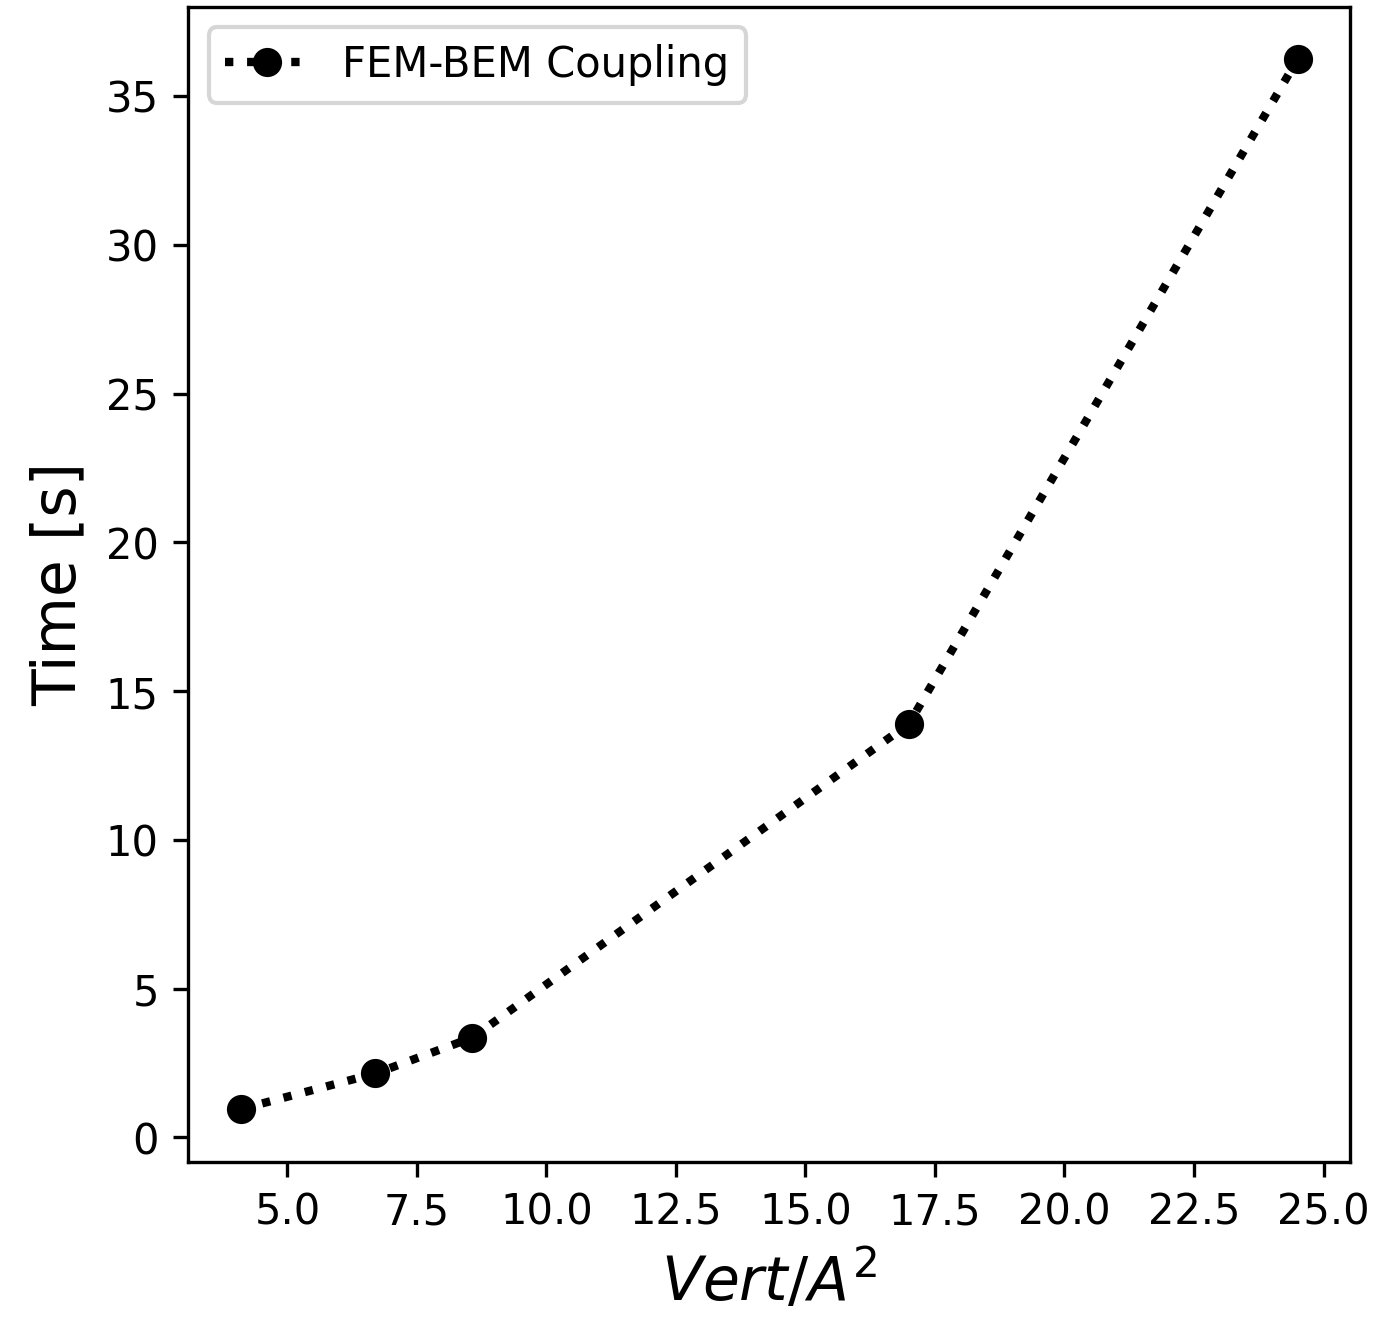
\includegraphics[width=0.45\linewidth]{DolfinX_Arginine2_varying_coeff_time.png}
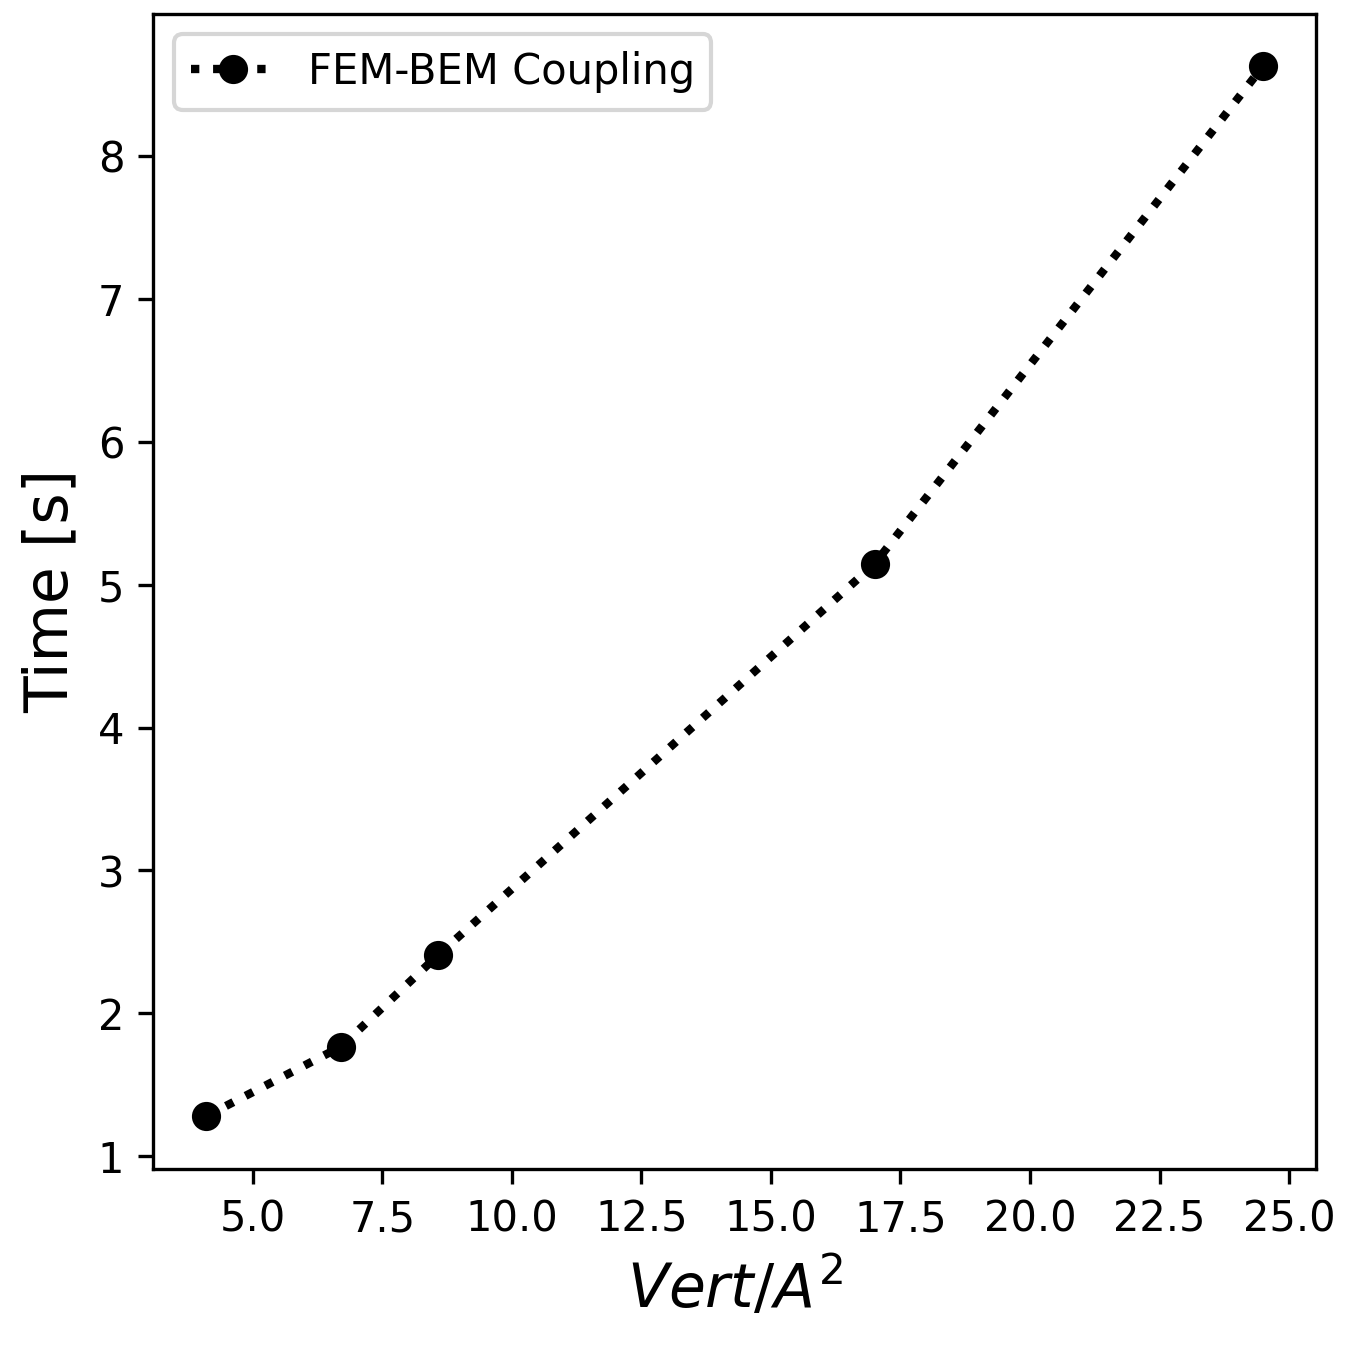
\includegraphics[width=0.45\linewidth]{DolfinX_Arginine2_varying_coeff_set_time.png}
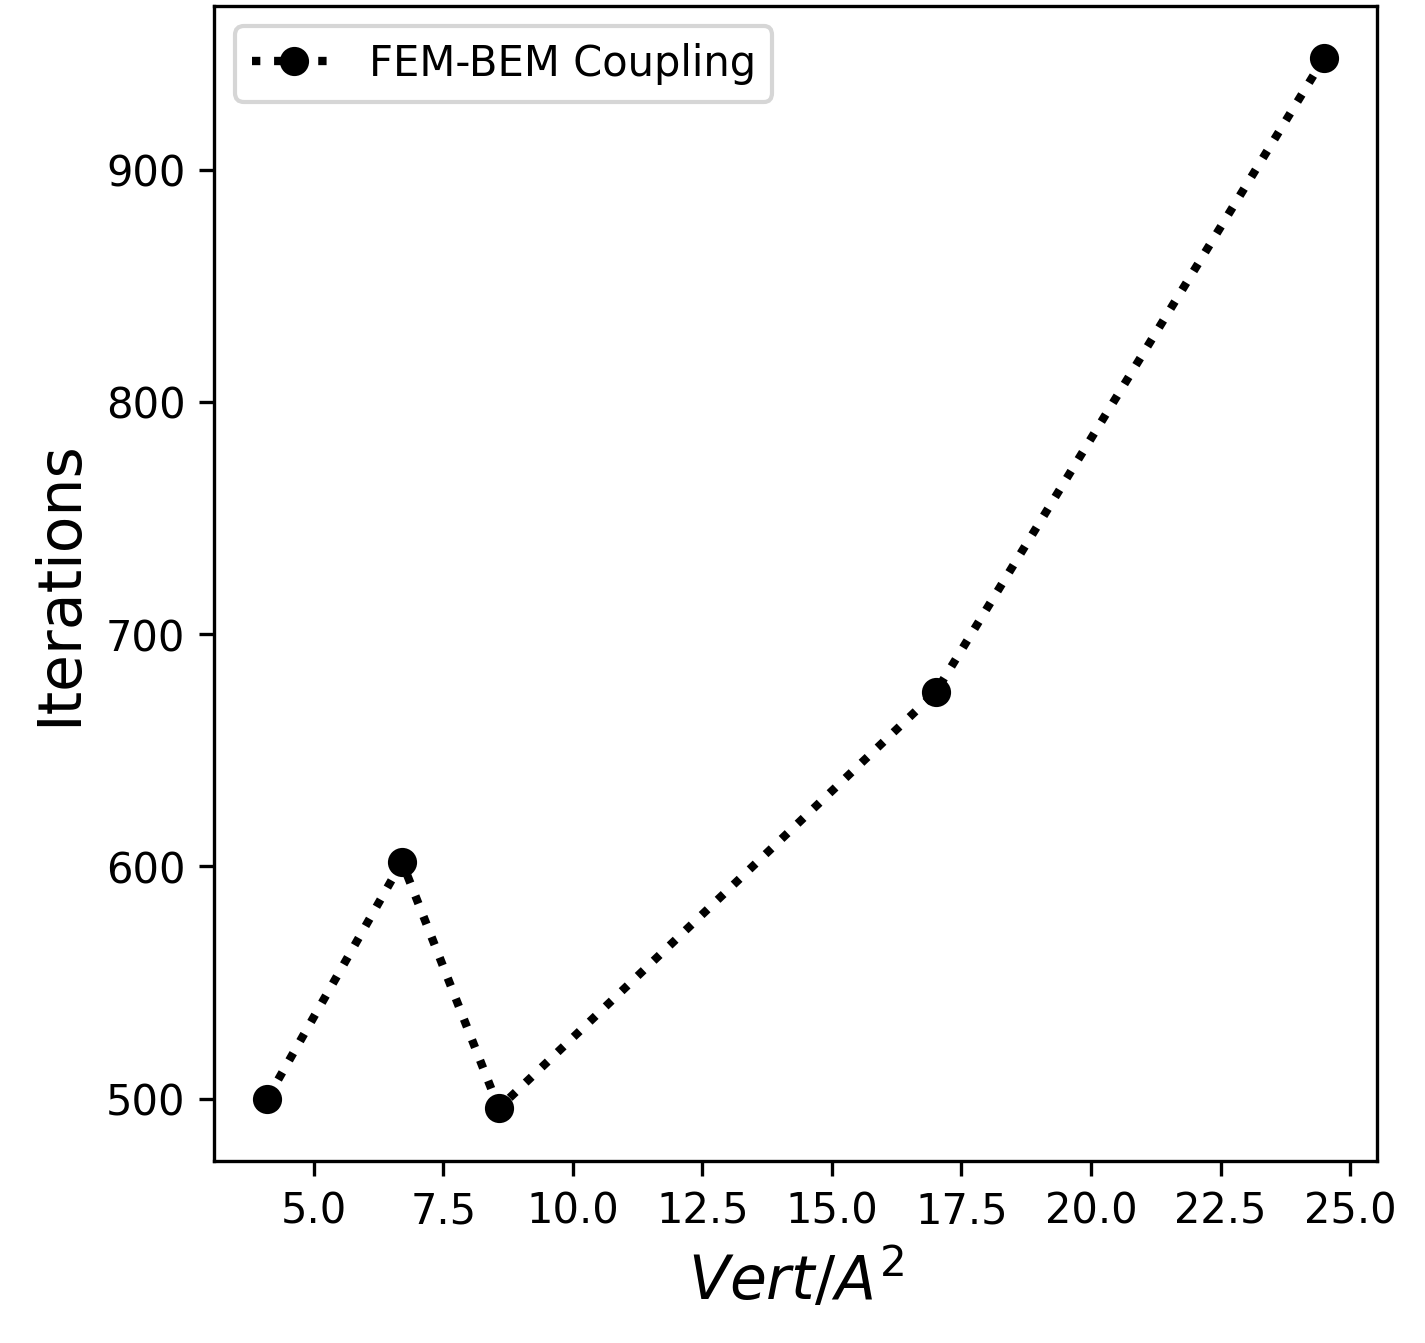
\includegraphics[width=0.45\linewidth]{DolfinX_Arginine2_varying_coeff_iter.png}
\caption{Iteration count and time-to-solution to compute the solvation energy of arginine with a variable permittivity (left: Online time taken to solve systems, right: Offline time taken to set up systems), using FEM-BEM coupling. %Can we make this only two plots?
}
\label{fig:arg2_variable}
\end{figure}


\subsection*{\sffamily \large Performance analysis for larger structures}

So far, we have only tested the FEM-BEM coupled approach with small structures. Here, we study its behaviour with larger structures to evaluate its applicability in more realistic settings, and  in test cases where BEM-BEM coupling is not an alternative. Using the same Gaussian permittivity field inside the molecule, we computed the solvation free energy of protein G B1 (955 atoms, PDB code 1pgb), lysozyme (1960 atoms, PDB code 1lyz), the barnase-barstar complex (9464 atoms, PDB code 1x1u), and immunoglobulin G (20148 atoms, PDB code 1igt). All structures were parameterized with the Amber\cite{Swanson05} force field using pdb2pqr.\cite{Dolinsky04} The surface was meshed with Nanoshaper\cite{decherchi2013general} considering a grid scale of 1.5, and then used to mesh the solute region with pyGAMer\cite{lee2020open} and TetGen\cite{hang2015tetgen} with a radius-edge ratio of 1.0. Solvation free energy and timings for these runs are presented in Table \ref{table:large_variable}, showing that our FEM-BEM coupling method can reach medium-to-large sized proteins on a workstation. 

Table \ref{table:large_variable} shows that the iteration count increases with the problem size. This is expected for Johnson-N\'ed\'elec, which is the simplest coupling strategy. To isolate the effect of the increased iterations in the analysis, we separate timings in ``setup'' and ``solving'' time, where the ``setup'' time is independent of the number of iterations, and the ``solving'' time corresponds to the time spent in the GMRES solver. Then, the time-per-iteration in table \ref{table:large_variable} only considers the ``solving'' time. Looking at the increase in degrees of freedom, which scales equivalently for FEM and BEM, the ``setup'' time scales slightly worse than $\mathcal{O}(N^2)$, mainly due to the dense nature of the BEM portion of the matrix \textcolor{red}{(check if not using fmm)}. On the other hand, the ``solving time per iteration'' scales closer to $\mathcal{O}(N)$. This is an indication that the high ``solving time'' is mainly due to the increase in iteration count, and having better conditioned coupling methods, such as the so-called hybrid approach,\cite{betcke2022hybrid} can have a large impact in the time to solution.

Even though this scheme is capable of calculating the electrostatic potential in medium-to-large proteins, the largest test case in Table \ref{table:large_variable} (1igt) used up most of the available RAM memory (\textcolor{red}{check and rewrite}). If we were aiming at larger structures, such as full viruses,\cite{MartinezETal2019,wang2021high} we would require to improve not only in the conditioning of the system, but also in the choice of fast algorithms\cite{Wantfmm,Betrckefmm} and parallelization.

\begin{table}
\centering
\resizebox{\textwidth}{!}{\begin{tabular}{c|c|c|c|c|c|c|c|c}
Molecule & FEM  & BEM &  $\Delta G_{solv}$ & Iterations & Setup Time & Solving Time & Solv. time per & Total Time \\
& DOFs & DOFs &  kcal/mol & & [sec] & [sec] & iter. [sec] & [sec] \\
\hline
 1pgb  & 29 434 &  10 058 &  -300.888 & 826 & 82 & 547 & 0.6 & 6 629  \\
 1lyz  & 56 114 & 18 606 &  -599.642 & 1 285 & 330 & 1 640  & 1.2 & 1 970  \\
 %1lyz gs3 & 257 391 & 75 048 &  -600.637 & 2 949  & 1 690 & 10 900 & 3.6 & 12 590   \\
 1x1u & 263 181 & 81 258 \textcolor{red}{82360} &  -1 984.468 & 4 167 & 8 240 & 16 300 & 3.91 & 24 540  \\
 1igt & 597 575 & 187 712 \textcolor{red}{189960} &   -3 294.230 & 8 361 & 41 200 & 64 200 & 7.67  &  105 400   \\
 \hline
\end{tabular}}
\caption{Results for larger structures with a variable permitivitty.}
\label{table:large_variable}
\end{table}
%
%\begin{table}
%\centering
%\begin{tabular}{c|c|c|c|c|c|c|c|c}
%Molecule & Mesh size  & FEM  & BEM &  $\Delta G_{solv}$ & Iterations & Setup Time & Solving Time & Total Time \\
%& vert/\AA$^2$ & DOFs & DOFs &  kcal/mol & & sec & sec & sec \\
%\hline
% 1pgb &  & 29 434 &  10 058 &  -300.888 & 826 & 82 & 547 & 629  \\
% 1lyz &  & 56 114 & 18 606 &  -599.642 & 1 285 & 330 & 1 640  & 1 970  \\
% 1lyz gs3 &  & 257 391 & 75 048 &  -600.637 & 2 949  & 1 690 & 10 900 & 12 590   \\
% 1uxu &  & 263 181 & 81 258 &  -1 984.468 & 4 167 & 8 240 & 16 300 & 24 540  \\
% 1igt &  & 597 575 & 187 712 &   -3 294.230 & 8 361 & 41 200 & 64 200 &  105 400   \\
% \hline
%\end{tabular}
%\caption{Large tests' results}
%\label{table:large_variable}
%\end{table}

%((Place Results here. Not needed for review articles.))

%\section*{\sffamily \Large First-order heading}
 
%((Equations should be inserted using standard LaTeX equation and eqnarray environments, not as graphics, and should be set in the main text))
%Equation											(1)
%((References should be superscripted and appear after punctuation.1,2 Please define all acronyms at their first usage except IR, UV, NMR, and DNA or similar commonly understood terms.)) 


%\subsection*{\sffamily \large Second-order heading}

%\subsubsection*{\sffamily \normalsize Third-order heading}

%{\sffamily \small Fourth-order heading}\\

%\section*{\sffamily \Large DISCUSSION}

%((Place Discussion here. Not needed for review articles.))


\section*{\sffamily \Large CONCLUSIONS}
This paper presents the first implementation of a FEM-BEM coupling approach to solve the Poisson--Boltzmann equation for molecular electrostatics. This brings the best of both worlds: the accuracy and efficiency of BEM to exactly enforce the boundary conditions at infinity, and the flexibility of FEM to account for space variations of the material properties and nonlinearities. After presenting verification results of solvation energy for a sphere and arginine with a constant permittivity inside the solute, and binding energy  for an extensive data set, we showcased our implementation with an advanced modeling technique that considers Gaussian-varying permittivities in a confined region, with the results validated against the widely-used APBS software. The final scaling results for larger molecules start from protein G B1 (955 atoms) and go up to immunoglobulin G (20\,148 atoms), proving the applicability of this approach for realistic problems. Even though our implementation was able to reach medium-to-large systems, we recongnize the need for further research towards better preconditioning of the linear system, optimizing the coupling technique, acceleration algorithms, and parallel execution, especially as we look towards much larger solutes, like viruses. We hope this proof-of-concept work will serve as motivation for future model development that considers space-varying permittivities and Debye lengths, and mixed linear-nonlinear techniques, especially for highly-charged systems, like nucleic acids. 

%((Place Conclusions here.))

\subsection*{\sffamily \large ACKNOWLEDGMENTS}

%((Place Acknowledgments here))


%((Additional Supporting Information may be found in the online version of this article.))

\clearpage

%%%%%%%%%%%%%%%%%%%%%%%%%%%%%%%%%%%%%%%%%%%%%%%%%%%%%%%%%%%%%%%%%%%%%%%%%%%%%%%%%
% BIBLIOGRAPHY

\bibliography{main}   % Produces the bibliography via BibTeX.

%\begin{thebibliography}{99}
%
%
%\bibitem{Coulson}
%Coulson, C. A., Rev. Mod. Phys., \textbf{1960}, 32,170-177.
%\bibitem{Malrieu}
%Malrieu, J.-P., J. Mol. Struct., \textbf{1998}, 424, 1-2,83-91.
%\bibitem{Shaik}
%Shaik, S., New. J. Chem., \textbf{2007}, 31,2015-2028.
%\bibitem{Hoffmann}
%Hoffman, R., Schleyer, P. v. R., Schaefer III, H. F., \textbf{2008}, 47, 7164-7167.
%\bibitem{Perdew}
%Perdew, J. P., Ruzsinszky, A., Constantin, L., Sun, J., Csonka, G., J. Chem. Theory Comput., \textbf{2009}, 5, 902-908.
%\bibitem{Koros}
%Koros, W. J.; Chern, R. T. In Handbook of Separation Process Technology; Rousseau, E. D.; Russell, B., Eds.; Wiley: New York, \textbf{1987}; Vol. 2, Chapter 20, pp 34-45.
%\end{thebibliography}


%%%%%%%%%%%%%%%%%%%%%%%%%%%%%%%%%%%%%%%%%%%%%%%%%%%%%%%%%%%%%%%%%%%%%%%%%%%%%%%%%

%\clearpage
%%%%%%%%%%%%%%%%%%%%%%%%%%%%%%%%%%%%%%%%%%%%%%%%%%%%%%%%%%%%%%%%%%%%%%%%%%%%%%%%%%
%% FIGURE CAPTIONS
%
%%%%%% FIGURE ---- cc.eps
%\begin{figure}
%\caption{\label{cc} Place Figure 1 caption here. In the case of reproduced figures in review articles, you must obtain the publisher's permission and state a suitable notice here along with a citation.}
%\end{figure}
%
%\begin{figure}
%\caption{\label{fig2} Place Figure 2 caption here. Figures should be uploaded as individual files, preferably .tif or .eps files, at high enough resolution (600 to 1200 dpi) to ensure clarity. Please see the author’s guide for more details and specifications. For high quality illustrations, we highly recommend the use of the TikZ package.}
%\end{figure}
%
%
%%%%%%%%%%%%%%%%%%%%%%%%%%%%%
%
%
%
%%%%%%%%%%%%%%%%%%%%%%%%%%%%%%%%%%%%%%%%%%%%%%%%%%%%%%%%%%%%%%%%%%%%%%%%%%%%%%%%%%
%% FIGURE FILES
%
%\clearpage
%
%%\vspace*{0.1in}   %%% FIGURE 1
%%\begin{center}
%%\includegraphics[width=0.2\columnwidth,keepaspectratio=true]{cc.eps}
%%\end{center}
%\vspace{0.25in}
%\hspace*{3in}
%{\Large
%\begin{minipage}[t]{3in}
%\baselineskip = .5\baselineskip
%Figure 1 \\
%Author A, Author B, Author C, Author D \\
%J.\ Comput.\ Chem.
%\end{minipage}
%}
%
%\clearpage
%
%\begin{table}
%\begin{tabular}{|c|c|c|c|}\hline
%\textbf{Quantity} & \textbf{Calculated} & \textbf{Observed} & \textbf{Error} \\ \hline
%  Density & 5.3 & 6.3 & Within limits \\ \hline
%  Optical magnification & 8.3 & 90.9 & Utterly unacceptable\! \\ \hline
%\end{tabular}
%\caption{\label{tbl1} Place table caption here.}
%\end{table}

\end{document}

